\documentclass[UTF8,11pt]{article}

  % Package for using the full page.
  \usepackage{fullpage}
  
  % Package for writing algorithms (why do we need this one?).
  \usepackage[linesnumbered,ruled,vlined]{algorithm2e}
  
  % Package for using colored texts.
  \usepackage[dvipsnames]{xcolor}
  
  % Pakcage for using multiple optional parameters in new commands.
  \usepackage{xargs}

  % Packages for writing comments and todo notes.
  \usepackage[colorinlistoftodos,prependcaption,textsize=tiny]{todonotes}
  \newcommandx{\unsure}[2][1=]
    {\todo[linecolor=red,backgroundcolor=red!25,
	bordercolor=red,#1]
	{#2}\xspace{}}
  \newcommandx{\change}[2][1=]
    {\todo[linecolor=blue,backgroundcolor=blue!25,
	bordercolor=blue,#1]
	{#2}\xspace{}}
  \newcommandx{\info}[2][1=]
    {\todo[linecolor=OliveGreen,backgroundcolor=OliveGreen!25,
	bordercolor=OliveGreen,#1]
	{#2}}
  \newcommandx{\improvement}[2][1=]
    {\todo[linecolor=Plum,backgroundcolor=Plum!25,bordercolor=Plum,#1]
	{#2}\xspace{}}
  \newcommandx{\thiswillnotshow}[2][1=]
    {\todo[disable,#1]
	{#2}\xspace{}}

  % What are there for?
  % Select what to do with todonotes: 
  % \usepackage[disable]{todonotes} % notes not showed
  % \usepackage[draft]  {todonotes} % notes showed

  % Select what to do with command \comment:  
  % \newcommand{\comment}[1]
      {}                                    %comment not showed
  \newcommand{\comment}[1]
    {\par {\bfseries \color{blue} #1 \par}} %comment showed
  
  % ams math packages.
  \usepackage{amsmath, amssymb, amsthm, mathtools,mathbbol,prftree}
  \usepackage{txfonts}
  
  % Declare a global counter for theorem environments:
  \newcounter{thmcounter}
  
  % Define new theorem styles and theorem environments.
  \theoremstyle{plain}
  
  \newtheorem{theorem}    [thmcounter]{Theorem}
  \newtheorem{corollary}  [thmcounter]{Corollary}
  \newtheorem{lemma}      [thmcounter]{Lemma}
  \newtheorem{proposition}[thmcounter]{Proposition}
  
  \theoremstyle{definition}
  
  \newtheorem{definition} [thmcounter]{Definition}
  \newtheorem{example}    [thmcounter]{Example}
  
  \theoremstyle{remark}
  
  \newtheorem{remark}     [thmcounter]{Remark}
  \newtheorem{notation}   [thmcounter]{Notation}
    
  % Package for changing fonts in the Verbatim environment:
  \usepackage{fancyvrb}
  
  % Package for writing captions for align environment:
  \usepackage{capt-of}
  
  % Package for URLs:
  \usepackage{hyperref}  
  
  % Package for tables:
  \usepackage[english]{babel}  
  
  % Package for quotations:
  \usepackage{csquotes}
  
  % Package for customizing lists environments:
  \usepackage{enumitem}
  
  % Package for writing long tables:
  \usepackage{longtable}
  
  % Package for graphics
  \usepackage{graphicx}
  
  \usepackage{xspace}
  \usepackage{caption}
  \usepackage{longtable}
  
  % Define ceiling and flooring symbols:
  \usepackage{mathtools}
  \DeclarePairedDelimiter{\ceil}{\lceil}{\rceil}
  \DeclarePairedDelimiter{\floor}{\lfloor}{\rfloor}

  % Package for underlining and strikethrough texts.
  \usepackage[normalem]{ulem}
  
  % Package for display-mode quotations.
  \usepackage{csquotes}
  
  % Define double-bracket [[P]]
  \usepackage{stmaryrd}
  \newcommand{\Bracket}[1]{\llbracket#1\rrbracket}
  
  % Package for writing natural proof deductions
  \usepackage{prftree}
  
  \usepackage{enumitem}
  
  % logic connectives
  \newcommand{\imp}{\to}
  \newcommand{\dimp}{\leftrightarrow}
  \newcommand{\ddd}{,\dots,}
  
  % contexts
  \newcommand{\CSub}[1]{C_{#1}}
  \newcommand{\Csigma}{\CSub{\sigma}}
  \newcommand{\Csigmai}{\CSub{\sigma,i}}
  \newcommand{\Csigmaapp}[1]{\CSub{\sigma}[#1]}
  \newcommand{\Csigmaiapp}[1]{\CSub{\sigma,i}[#1]}
  \newcommand{\Capp}[1]{C[#1]}
  
  % name of the proof rules
  \newcommand{\prule}[1]{\textsc{(#1)}}
  
  \newcommand{\modusponens}{\prule{Modus Ponens}\xspace}
  \newcommand{\universalgeneralization}{\prule{Universal Generalization}\xspace}
  \newcommand{\necessitation}{\prule{Necessitation}\xspace}
  \newcommand{\existence}{\prule{Existence}\xspace}
  \newcommand{\singletonvariable}{\prule{Singleton Variable}\xspace}
  \newcommand{\propagationbottom}{\prule{Propagation$_\bot$}\xspace}
  \newcommand{\propagationvee}{\prule{Propagation$_\vee$}\xspace}
  \newcommand{\propagationexists}{\prule{Propagation$_\exists$}\xspace}
  \newcommand{\variablesubstitution}{\prule{Variable Substitution}\xspace}
  \newcommand{\framing}{\prule{Framing}\xspace}
  \newcommand{\propositionaltautology}{\prule{Propositional Tautology}\xspace}
  \newcommand{\forallrule}{\prule{$\forall$}\xspace}
  \newcommand{\membership}{\prule{Membership}\xspace}
  \newcommand{\membershipintroduction}{\prule{Membership Introduction}\xspace}
  \newcommand{\membershipelimination}{\prule{Membership Elimination}\xspace}
  \newcommand{\membershipneg}{\prule{Membership$_\neg$}\xspace}
  \newcommand{\membershipwedge}{\prule{Membership$_\wedge$}\xspace}
  \newcommand{\membershipexists}{\prule{Membership$_\exists$}\xspace}
  \newcommand{\equalityelimination}{\prule{Equality Elimination}\xspace}
  \newcommand{\membershipsymbol}{\prule{Membership Symbol}\xspace}
  \newcommand{\membershipvariable}{\prule{Membership Variable}\xspace}
  \newcommand{\functionalsubstitution}{\prule{Functional Substitution}\xspace}
    
  % Package for writing BNF syntax
  \usepackage{syntax}
  
  % Package for lstlisting and definition of Kore
  \usepackage{listings}
  % Define colors
  \definecolor{codegray}{rgb}{0.5,0.5,0.5}
  \definecolor{backgray}{RGB}{250,250,250}
  \definecolor{codegreen}{RGB}{50,205,50}
  \definecolor{codeblue}{RGB}{50,50,255}
  % Define Kore Language style
  \lstdefinelanguage{kore}
  {
  	% print whole listing small and in serif fonts
  	basicstyle=\ttfamily\footnotesize,
  	% use /* */ for comments
  	morecomment=[s]{/*}{*/},
  	% print white for comments
  	commentstyle=\color{codegray},
  	% print line number in the left, in tiny fonts
  	numbers=left,
  	numberstyle=\tiny,
  	% print all characters at their natural width
  	columns=fullflexible,
  	% print background color grey
  	backgroundcolor=\color{backgray},
  	% regard some characters as letters
  	alsoletter={-\#\\},
  	% list of declaration keywords
  	keywordstyle=[1]\color{codeblue},
  	morekeywords=[1]{
  		module,
  		endmodule,
  		hooked-sort,
  		sort,
  		symbol,
  		hooked-symbol,
  		alias,
  		axiom,
  	},
    % list of connectives
    keywordstyle=[2]\color{codegreen},
    morekeywords=[2]{
    	\\not,
    	\\or,
    	\\implies,
    	\\and,
    	\\equals,
    	\\exists,
    	\\forall,
    	\\iff
    }
  }

  % Define |-fin
  \newcommand{\vdashfin}{\vdash_\text{fin}}

  % Define the colon ":" that is used in "x:s"
  % with less spacing around.
  \newcommand{\cln}{\texttt{:}}

  % Define the curly K:
  \newcommand{\K}{\mbox{$\mathbb{K}$}\xspace}
  
  % Define commands that are used in Sec 2.  
  \newcommand{\Nat}{\textit{Nat}}
  \newcommand{\String}{\textit{String}}
  \newcommand{\Rat}{\textit{Rat}}
  \newcommand{\KNat}{\textit{KNat}}
  \newcommand{\Int}{\textit{Int}}
  \newcommand{\Bool}{\textit{Bool}}
  \newcommand{\List}{\textit{List}}
  \newcommand{\KList}{\textit{KList}}
  \newcommand{\nil}{\textit{nil}}
  \newcommand{\cons}{\textit{cons}}
  \newcommand{\append}{\textit{append}}
  \newcommand{\Bag}{\textit{Bag}}
  \newcommand{\Set}{\textit{Set}}
  \newcommand{\Map}{\textit{Map}}
  \newcommand{\emptyMap}{\textit{empty}}
  \newcommand{\bindMap}{\textit{bind}}
  \newcommand{\mergeMap}{\textit{merge}}
  \newcommand{\ittrue}{\textit{true}}
  \newcommand{\itfalse}{\textit{false}}
  \newcommand{\itceil}{\textit{ceil}}
  
  \newcommand{\Pred}{\textit{Pred}}
  
  \newcommand{\wnext}{{\medcirc}}
  \newcommand{\snext}{{\medbullet}}

  \newcommand{\Context}{\textit{Context}}
  \newcommand{\hole}{\boxempty}
  \newcommand{\Exp}{\textit{Exp}}
  \newcommand{\AExp}{\textit{AExp}}
  \newcommand{\BExp}{\textit{BExp}}
  \newcommand{\Stmt}{\textit{Stmt}}
  \newcommand{\ite}{\textsf{ite}}
  \newcommand{\ttrue}{\textit{true}}
  \newcommand{\ffalse}{\textit{false}}
  \newcommand{\app}{\textit{app}}
  \newcommand{\KExp}{\mathit{\#Exp}}
  \newcommand{\Klambdazero}{\mathit{Klambda0}}
  \newcommand{\Kapp}{\mathit{Kapp}}
  \newcommand{\Klambda}{\mathit{Klambda}}
  \newcommand{\parametric}[2]{{#1}\raisebox{.2ex}{\texttt{\footnotesize{\{}}}#2\raisebox{.2ex}{\texttt{\footnotesize{\}}}}}
  \newcommand{\parametricscript}[2]{{#1}\raisebox{.2ex}{\texttt{\tiny{\{}}}#2\raisebox{.2ex}{\texttt{\tiny{\}}}}}
  
  \newcommand{\zero}{\textit{zero}}
  \newcommand{\Kzero}{\textit{Kzero}}
  \newcommand{\Ksucc}{\textit{Ksucc}}
  \newcommand{\KSymbolsucc}{\textit{KSymbolsucc}}
  \newcommand{\Mod}{\textit{Mod}}
  \newcommand{\denote}[1]{\llbracket{#1}\rrbracket}
  \newcommand{\reduct}[2]{\mbox{${#1}\!\!\upharpoonright_{#2}$}}
  \newcommand{\reductscript}[2]{\mbox{\tiny${#1}\!\!\upharpoonright_{#2}$}}
  
  \newcommand{\isEmpty}{\textit{isEmpty}}
  
  \newcommand{\ostoml}{\textsf{os2ml}}
  
  \newcommand{\builtin}{\textit{builtin}}
  
  % Define PATTERNS with ATTERNS are small capitals:
  \newcommand{\PATTERNS}{\text{P\textsc{atterns}}}
  \newcommand{\VARIABLES}{\text{V\textsc{ariables}}}
  % Define sorts and symbols in the calculus K.
  
  \newcommand{\doubleslash}{/\!/{ }}
  
  \newcommand{\compose}{\circ}
  \newcommand{\strict}[1]{\textsf{strict(#1)}}

  \newcommand{\shp}{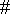
\includegraphics{hash-symbol}\kern-0.1em}
  \newcommand{\smallshp}{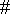
\includegraphics[scale=0.8]{hash-symbol}\kern-0.1em}
  \newcommand{\sharpsymbol}{\#}
  \newcommand{\shs}{\shp s}
  \newcommand{\shvs}{\shp vs}
  \newcommand{\smallshs}{\smallshp s}
  \newcommand{\sharpup}{\texttt{\sharpsymbol up}}
  \newcommand{\sharpdown}{\texttt{\sharpsymbol down}}
  % Sec 3.1 Truth
  \newcommand{\KPred}{\mathit{\shp Pred}}
  
  % Sec 3.2 Strings
  \newcommand{\KChar}{\texttt{\sharpsymbol Char}}
  \newcommand{\KCharList}{\texttt{\sharpsymbol CharList}}
  \newcommand{\KString}{\texttt{\sharpsymbol String}}
  \newcommand{\Kepsilon}{\texttt{\sharpsymbol epsilon}}
  \newcommand{\KconsKString}{\texttt{\sharpsymbol consKString}}
  
  %% We shouldn't need the follows.  
  \newcommand{\Kconcat}{\texttt{\sharpsymbol concat}}
  
  \newcommand{\Kconstructor}{\texttt{\sharpsymbol constructor}}
  \newcommand{\KconstructorP}[1]{\parametric{\Kconstructor}{#1}}
  \newcommand{\Kinjective}{\texttt{\sharpsymbol injective}}
  \newcommand{\KinjectiveP}[1]{\parametric{\Kinjective}{#1}}
  
  \newcommand{\KprovableP}[1]{\parametric{\Kdeduce}{#1}}
  
  % Sec 3.3 Sorts and Symbols
  \newcommand{\KSort}{\texttt{\sharpsymbol Sort}}
  \newcommand{\Ksort}{\texttt{\sharpsymbol sort}}
  \newcommand{\KSymbol}{\texttt{\sharpsymbol Symbol}}
  \newcommand{\Ksymbol}{\texttt{\sharpsymbol symbol}}
  \newcommand{\KSymbolceil}{\texttt{\sharpsymbol `ceil}}
  \newcommand{\KgetArgumentSorts}{\texttt{\sharpsymbol getArgumentSorts}}
  \newcommand{\KgetReturnSort}{\texttt{\sharpsymbol getReturnSort}}
  
  % Sec 3.4 Finite Lists
  \newcommand{\ttX}{\texttt{X}}
  \newcommand{\ttChar}{\texttt{Char}}
  \newcommand{\ttSort}{\texttt{Sort}}
  \newcommand{\ttSymbol}{\texttt{Symbol}}
  \newcommand{\ttVariable}{\texttt{Variable}}
  \newcommand{\ttPattern}{\texttt{Pattern}}
  \newcommand{\XList}{\texttt{\sharpsymbol XList}}
  \newcommand{\KnilXList}{\texttt{\sharpsymbol nilXList}}
  \newcommand{\KconsXList}{\texttt{\sharpsymbol consXList}}
  \newcommand{\KappendXList}{\texttt{\sharpsymbol appendXList}}
  \newcommand{\KinXList}{\texttt{\sharpsymbol inXList}}
  \newcommand{\KdeleteXList}{\texttt{\sharpsymbol deleteXList}}
  \newcommand{\KPatternList}{\texttt{\sharpsymbol PatternList}}
  \newcommand{\KnilKPatternList}{\texttt{\sharpsymbol nilPatternList}}
  \newcommand{\KconsKPatternList}{\texttt{\sharpsymbol consPatternList}}
  \newcommand{\KappendKPatternList}{\texttt{\sharpsymbol appendPatternList}}
  \newcommand{\KinKPatternList}{\texttt{\sharpsymbol inPatternList}}
  \newcommand{\KdeleteKPatternList}{\texttt{\sharpsymbol deletePatternList}}
  \newcommand{\KSortList}{\texttt{\sharpsymbol SortList}}
  \newcommand{\KnilKSortList}{\texttt{\sharpsymbol nilSortList}}
  \newcommand{\KconsKSortList}{\texttt{\sharpsymbol consSortList}}
  \newcommand{\KappendKSortList}{\texttt{\sharpsymbol appendSortList}}
  \newcommand{\KinKSortList}{\texttt{\sharpsymbol inSortList}}
  \newcommand{\KdeleteKSortList}{\texttt{\sharpsymbol deleteSortList}}
  \newcommand{\KnilKSymbolList}{\texttt{\sharpsymbol nilSymbolList}}
  \newcommand{\KconsKSymbolList}{\texttt{\sharpsymbol consSymbolList}}
  \newcommand{\KSymbolList}{\texttt{\sharpsymbol SymbolList}}
  \newcommand{\KappendKSymbolList}{\texttt{\sharpsymbol appendSymbolList}}
  \newcommand{\KinKSymbolList}{\texttt{\sharpsymbol inSymbolList}}
  \newcommand{\KdeleteKSymbolList}{\texttt{\sharpsymbol deleteSymbolList}}
  \newcommand{\KnilKCharList}{\texttt{\sharpsymbol nilCharList}}
  \newcommand{\KconsKCharList}{\texttt{\sharpsymbol consCharList}}
  \newcommand{\KVariableList}{\texttt{\sharpsymbol VariableList}\xspace}
  \newcommand{\KnilKVariableList}{\texttt{\sharpsymbol nilVariableList}}
  \newcommand{\KconsKVariableList}{\texttt{\sharpsymbol consVariableList}}
  \newcommand{\KinKVariableList}{\texttt{\sharpsymbol inVariableList}}
  \newcommand{\KappendKVariableList}{\texttt{\sharpsymbol appendVariableList}}
  \newcommand{\KdeleteKVariableList}{\texttt{\sharpsymbol deleteVariableList}}
  \newcommand{\KappendKCharList}{\texttt{\sharpsymbol appendKCharList}}
  \newcommand{\KVariable}{\texttt{\sharpsymbol Variable}}
  \newcommand{\KVariableAsKPattern}{\texttt{\sharpsymbol variableAsPattern}}
  \newcommand{\KvariablePattern}{\texttt{\sharpsymbol variablePattern}}
  \newcommand{\KPattern}{\texttt{\sharpsymbol Pattern}}
  \newcommand{\Kvariable}{\texttt{\sharpsymbol variable}}
  \newcommand{\Kand}{\texttt{\sharpsymbol  \slashsymbol and}}
  \newcommand{\Kor}{\texttt{\sharpsymbol \slashsymbol  or}}
  \newcommand{\Kimplies}{\texttt{\sharpsymbol  \slashsymbol implies}}
  \newcommand{\Kiff}{\texttt{\sharpsymbol  \slashsymbol iff}}
  \newcommand{\Knot}{\texttt{\sharpsymbol  \slashsymbol not}}
  \newcommand{\Kapplication}{\texttt{\sharpsymbol application}}
  \newcommand{\Kexists}{\texttt{\sharpsymbol \slashsymbol  exists}}
  \newcommand{\Kforall}{\texttt{\sharpsymbol \slashsymbol  forall}}
  \newcommand{\Kequals}{\texttt{\sharpsymbol \slashsymbol  equals}}
  \newcommand{\Kmembership}{\Kin}
  \newcommand{\Kin}{\texttt{\sharpsymbol \slashsymbol  in}}
  \newcommand{\Kcontains}{\texttt{\sharpsymbol  \slashsymbol contains}}
  \newcommand{\Ktop}{\texttt{\sharpsymbol \slashsymbol  top}}
  \newcommand{\Kbottom}{\texttt{\sharpsymbol \slashsymbol  bottom}}
  \newcommand{\Kfloor}{\texttt{\sharpsymbol \slashsymbol  floor}}
  \newcommand{\Kceil}{\texttt{\sharpsymbol \slashsymbol  ceil}}
  \newcommand{\Knext}{\texttt{\sharpsymbol \slashsymbol next}}
  \newcommand{\Krewrites}{\texttt{\sharpsymbol \slashsymbol rewrites}}
  
  \newcommand{\KVariableListAsKPatternList}
    {\texttt{\sharpsymbol variableListAsPatternList}\xspace}
  
  \newcommand{\Kdv}{\texttt{\sharpsymbol \slashsymbol dv}}
  
  \newcommand{\KgetFV}{\texttt{\sharpsymbol getFV}}
  \newcommand{\KgetFVFromPatterns}{\texttt{\sharpsymbol getFVFromPatterns}}
  \newcommand{\KoccursFree}{\texttt{\sharpsymbol occursFree}}
  \newcommand{\KfreshName}{\texttt{\sharpsymbol freshName}}
  \newcommand{\Kcons}{\texttt{\sharpsymbol cons}}
  \newcommand{\Knil}{\texttt{\sharpsymbol nil}}
  \newcommand{\KSymbolzero}{\texttt{\sharpsymbol Symbolzero}}
  \newcommand{\KSymbolcons}{\texttt{\sharpsymbol Symbolcons}}
  \newcommand{\KSymbolnil}{\texttt{\sharpsymbol Symbolnil}}
  
  \newcommand{\KSignature}{\texttt{\sharpsymbol Signature}}
  \newcommand{\Ksignature}{\texttt{\sharpsymbol signature}}
  \newcommand{\KgetSorts}{\texttt{\sharpsymbol getSorts}}
  \newcommand{\KgetSymbols}{\texttt{\sharpsymbol getSymbols}}
  \newcommand{\KsortDeclared}[1]{
  	\parametric{\texttt{\sharpsymbol sortDeclared}}{#1}}
  \newcommand{\KsortsDeclared}[1]{
        \parametric{\texttt{\sharpsymbol sortsDeclared}}{#1}}
  \newcommand{\KsymbolDeclared}[1]{
  	\parametric{\texttt{\sharpsymbol symbolDeclared}}{#1}}
  \newcommand{\KaxiomDeclared}{\texttt{\sharpsymbol axiomDeclared}}
  \newcommand{\Kderivable}{\Kdeduce}
  
  \newcommand{\Ksubsort}[1]{\parametric{\texttt{\sharpsymbol subsort}}{#1}}
  \newcommand{\Ksubsorts}[1]{\parametric{\texttt{\sharpsymbol subsorts}}{#1}}
  \newcommand{\KSortConnectedComponent}{\texttt{\sharpsymbol 
  SortConnectedComponent}}
  \newcommand{\KsubsortOverloading}[1]{
  	\parametric{\texttt{\sharpsymbol subsortOverloading}}{#1}}
  
  \newcommand{\KwellFormed}{\texttt{\sharpsymbol wellFormed}}
  \newcommand{\KwellFormedPatterns}{\texttt{\sharpsymbol wellFormedPatterns}}
  \newcommand{\KgetSort}{\texttt{\sharpsymbol getSort}}
  \newcommand{\KgetSortsFromPatterns}{\texttt{\sharpsymbol 
  getSortsFromPatterns}}
  \newcommand{\KisSort}{\texttt{\sharpsymbol isSort}}
  \newcommand{\Ksubstitute}{\texttt{\sharpsymbol substitute}}
  \newcommand{\KsubstitutePatterns}{\texttt{\sharpsymbol substitutePatterns}}
  
  \newcommand{\KTheory}{\texttt{\sharpsymbol Theory}}
  \newcommand{\Ktheory}{\texttt{\sharpsymbol theory}}
  \newcommand{\KwellFormedTheory}{\texttt{\sharpsymbol wellFormedTheory}}
  
  \newcommand{\Kdeduce}{\textup{\texttt{\sharpsymbol provable}}}
  
  \newcommand{\Ksc}[1]{\parametric{\textup{\texttt{\sharpsymbol sc}}}{#1}}
  
  % The italic font of "ceil" used in math mode.
  \newcommand{\cl}{\mathit{ceil}}
  
  \newcommand{\doublecolon}{::}
  % Use quotation marks "..." in math mode.
  \newcommand{\quot}[1]{\mathrm{``#1"}}
  \newcommand{\quottt}[1]{\textrm{\lq\texttt{#1}\rq}}
  \newcommand{\qquottt}[1]{\textrm{``\texttt{#1}''}}

  \newcommand{\Pattern}{\textsc{Pattern}\xspace}
  \newcommand{\ra}{\rightarrow}
  \newcommand{\lra}{\leftrightarrow}
  \newcommand{\FV}{{\it FV}}
  
  \newcommand{\name}{\mathit{name}}
  \newcommand{\llist}{\mathit{list}}
  \newcommand{\smalltt}[1]{\texttt{\small #1} }
  \newcommand{\sort}{\smalltt{sort}}
  \newcommand{\symb}{\smalltt{symbol}}
  \newcommand{\axiom}{\smalltt{axiom}}
  
  \newcommand{\inj}[2]{\parametric{\mathit{inj}}{#1, #2}}
  \newcommand{\retract}[2]{\parametric{\mathit{retract}}{#1, #2}}
  \newcommand{\factorial}{\textit{factorial}}
  % User-defined sorts & symbols in the meta-theory
  \newcommand{\KqNat}{\texttt{\shp `Nat}{ }}
  \newcommand{\KqList}{\texttt{\shp `List}{ }}
  \newcommand{\Kqzero}{\texttt{\shp `zero}{ }}
  \newcommand{\Kqsucc}{\texttt{\shp `succ}{ }}
  \newcommand{\Kqplus}{\texttt{\shp `plus}{ }}
  \newcommand{\Kqnil}{\texttt{\shp `nil}{ }}
  \newcommand{\Kqcons}{\texttt{\shp `cons}{ }}
  \newcommand{\Kqappend}{\texttt{\shp `append}{ }}
  \newcommand{\KqK}{\texttt{\shp `K}{}}
  \newcommand{\Kqinj}{\texttt{\shp `inj}}
  
  % Define the slash symbol
  \newcommand{\slashsymbol}{\symbol{92}}
  % Define slashed ttfamily words
  \newcommand{\slsh}[1]{\texttt{\slashsymbol#1}}
  \newcommand{\sland}{\slsh{and}}
  \newcommand{\slor}{\slsh{or}}
  \newcommand{\slnot}{\slsh{not}}
  \newcommand{\slimplies}{\slsh{implies}}
  \newcommand{\sliff}{\slsh{iff}}
  \newcommand{\slequals}{\slsh{equals}}
  \newcommand{\slexists}{\slsh{exists}}
  \newcommand{\slforall}{\slsh{forall}}
  \newcommand{\sltop}{\slsh{top}}
  \newcommand{\slbottom}{\slsh{bottom}}
  \newcommand{\slceil}{\slsh{ceil}}
  \newcommand{\slfloor}{\slsh{floor}}
  \newcommand{\slin}{\slsh{in}}
  \newcommand{\slnext}{\slsh{next}}
  \newcommand{\slrewrites}{\slsh{rewrites}}
  
  \newcommand{\sldv}{\slsh{dv}}
  
  \newcommand{\itlogic}{\mathit{logic}}
  \newcommand{\itconnective}{\mathit{connective}}
  \newcommand{\itsort}{\mathit{sort}}
  \newcommand{\itsymbol}{\mathit{symbol}}
  \newcommand{\itdeclared}{\mathit{declared}}
  \newcommand{\itsortDeclared}{\mathit{sortDeclared}}
  \newcommand{\collapse}{\mathit{collapse}}
  
  \newcommand{\ttv}{\texttt{v}}
  \newcommand{\ttp}{\texttt{p}}
  \newcommand{\itvp}{\mathit{vp}}
  
  \newcommand{\att}{\mathit{att}}
  \newcommand{\verbose}{\mathit{verbose}}
  \newcommand{\var}{\mathit{var}}
  

  
  % Define syntactic category <category>
  \newcommand{\syntacc}[1]{\text{$\langle$\textit{#1}$\rangle$}}

  % Title and authors
  \title{The Semantics of \K}
  \author{Formal Systems Laboratory \\
          University of Illinois at Urbana-Champaign}

\begin{document}

\maketitle

\info[inline]{Please feel free to contribute to this report in all ways.
You could add new contents, remove redundant ones, refactor and
organize the texts, and correct typos, but please follow the FSL
rules for editing, though; e.g., $<$80 characters per line,
each sentence on a new line, etc. }

\tableofcontents

\section{Introduction}
\label{sec:introduction}

\K is a best effort realization of matching logic~\cite{rosu-2017-lmcs}.
Matching logic allows us to mathematically define arbitrarily infinite
theories, which are not in general possible to describe finitely.
\K proposes a finitely describable subset of matching logic theories.
Since its inception in 2003 as a notation within
Maude~\cite{clavel-et-al99a} convenient for teaching programming
languages~\cite{rosu-2003-cs322}, until recently \K's semantics was explained
either by translation to rewriting logic \cite{meseguer-1992-tcs} or by
translation to some form of graph rewriting~\cite{serbanuta-rosu-2012-icgt}.
These translations not only added clutter and came at a loss of part of the
intended meaning of \K, but eventually turned out to be a serious limiting
factor in the types of theories and languages that could be defined.
Matching logic was specifically created and developed to serve as a
logical, semantic foundation for \K, after almost 15 years of experience
with using \K to define the formal semantics of real-life programming
languages, including
C~\cite{ellison-rosu-2012-popl,hathhorn-ellison-rosu-2015-pldi},
Java~\cite{bogdanas-rosu-2015-popl},
JavaScript~\cite{park-stefanescu-rosu-2015-pldi},
Python~\cite{guth-2013-thesis,pltredex-python},
PHP~\cite{k-php},
EVM~\cite{hiraidefining,hildenbrandt-saxena-zhu-rodrigues-daian-guth-rosu-2017-tr}.

Matching logic allows us to define \emph{theories} $(S,\Sigma,A)$ consisting
of potentially infinite sets of \emph{sorts} $S$, of \emph{symbols}
$\Sigma$ over sorts in $S$ (also called $S$-symbols), and of \emph{patterns}
$A$ built with symbols in $\Sigma$ (also called $\Sigma$-patterns),
respectively, and provides models that interpret the symbols
relationally, which in turn yield a \emph{semantic validity} relation
$(S,\Sigma,A)\models\varphi$ between theories $(S,\Sigma,A)$ and
$\Sigma$-patterns $\varphi$.
Matching logic also has a Hilbert-style complete proof system, which allows
us to derive new patterns $\varphi$ from given theories $(S,\Sigma,A)$,
written $(S,\Sigma,A)\vdash\varphi$.
When the sorts and signature are understood, we omit them; for example,
the completeness of matching logic then states that for any matching logic
theory $(S,\Sigma,A)$ and any $\Sigma$-pattern $\varphi$, we have
$A \models \varphi$ iff $A \vdash \varphi$.

...\improvement{Will add more here as we finalize the notation.
we need some convincing example.  Maybe parametric maps?}
...\improvement{Bring some motivational arguments here why this is
all important.  Why do we want to define the semantics of \K by going
to the meta-level.  Why people who just want to implement \K tools should
be interested in this document.}

\section{Matching Logic}
\label{sec:matching-logic}

\newcommand{\Var}{\textit{Var}}
\newcommand{\Name}{\textit{Name}}

In this section we first recall basic matching logic syntax and semantics
notions from~\cite{rosu-2017-lmcs} at a theoretical level.
Then we discuss schematic/parametric ways to finitely define infinite
matching logic theories.
Finally, we introduce theoretical foundations underlying the
notion of ``builtins''.


\subsection{Syntax}
\label{sec:ML-syntax}
Assume a matching logic \emph{signature} $(S, \Sigma)$, where $S$ is the
set of its \emph{sorts} and $\Sigma$ is the set of its \emph{symbols}.
When $S$ is understood, we write just $\Sigma$ for a signature instead of
$(S,\Sigma)$.
Assume a set {\Name} of infinitely many \emph{variable names}.
We partition $\Sigma$ in sets $\Sigma_{s_1 \ldots s_n, s}$, where
$s_1,\ldots, s_n, s \in S$.
The formulae of matching logic are called \emph{patterns}, although we
may also call them \emph{formulae}.
The set $\Pattern_s$ of patterns of sort $s \in S$ is generated by the
following grammar:
\begin{align*}
\varphi_s \Coloneqq\  &x \cln s \quad \text{where $x \in \Name$ and $s \in S$} 
& \textrm{// variable}
\\
\mid\  &\sigma(\varphi_{s_1},...,\varphi_{s_n}) \quad\
\text{where $\sigma \in \Sigma_{s_1 \ldots s_n, s}$ and
$\varphi_{s_1},...,\varphi_{s_n}$ of appropriate sorts}
& \textrm{// structure}
\\
\mid\  &\varphi_s \wedge_s \varphi_s 
& \textrm{// intersection}
\\
\mid\  &\neg_s \,\varphi_s
& \textrm{// complement}
\\
\mid\  &\exists_s \,x \cln s' .\, \varphi_s \quad \text{where $x \in N$ and $s' \in S$}
& \textrm{// binder}
\end{align*}
\begingroup\vspace*{-\baselineskip}
\captionof{figure}{The grammar of matching logic patterns.
For each $s\in S$, $\varphi_s$ are \emph{patterns of sort $s$}.}
\label{ml-grammar}
\vspace*{\baselineskip}\endgroup

Instead of writing $x \cln s$, we write just $x$ for a variable when $s$ is 
understood from the context or irrelevant.
Similarly, we omit the subscript $s$ of $\wedge_s$, $\neg_s$, and respectively
$\exists_s$ when understood from context or irrelevant.
Given a symbol $\sigma \in \Sigma_{s_1 \ldots s_n,s}$, $s_1 \ldots s_n$ are 
called the \emph{argument sorts} of $\sigma$, $s$ is called the 
\emph{return sort} of $\sigma$, and $n$ is called the \emph{arity} of
$\sigma$.
By abuse of language, we take the freedom to identify symbols
$\sigma\in\Sigma_{s_1 \ldots s_n,s}$ with corresponding patterns
$\sigma(x_1\cln s_1,...,x_n\cln s_n)$, where $x_1$, ..., $x_n$ are all
distinct names.
When $n = 0$, we call $\sigma$ a \emph{constant symbol} or simply a 
\emph{constant}.
If $\sigma$ is a constant, we write the pattern just $\sigma$ instead of 
$\sigma()$ for 
simplicity.

Let \Pattern be the $S$-sorted set of patterns $\{\Pattern_s\}_{s\in S}$.
The grammar above can be infinite, i.e., can have infinitely many
non-terminals and productions, because $S$ and $\Sigma$ can be
infinite.
Also, as usual, it only defines the syntax of formulae and not
their semantics.
For example, patterns $x \wedge y$ and $y \wedge x$ are distinct elements in
the language of the grammar, in spite of them being semantically/provably
equal in matching logic, as seen shortly.
For notational convenience, we take the liberty to use mix-fix syntax for
operators in $\Sigma$ and parentheses for grouping.
Also, recall that we may omit the sort of a variable when understood.
For example, if $\Nat \in S$ and
$\_+\_, \_*\_ \in \Sigma_{\Nat \times \Nat, \Nat}$
then we may write ``$(x + y)*z$'' instead of
``$\_*\_(\_+\_(x\cln\Nat,y\cln\Nat),z\cln\Nat)$''.
More notational conventions will be introduced along the way
as we use them. 
We adopt the following derived constructs (``syntactic sugar''): %\vspace*{-1ex}
$$\begin{array}{rcl@{\hspace*{10ex}}rcl}
\top_{\!\!s} & \equiv & \exists x\!:\!s \,.\, x &
\varphi_1 \ra \varphi_2 & \equiv & \neg\varphi_1 \vee \varphi_2 \\
\bot_{s} & \equiv & \neg \top_{\!\!s} &
\varphi_1 \lra \varphi_2 & \equiv & (\varphi_1 \ra \varphi_2) \wedge
 (\varphi_2 \ra \varphi_1) \\
\varphi_1 \vee \varphi_2 & \equiv & \neg(\neg\varphi_1\wedge\neg\varphi_2) &
\forall x . \varphi & \equiv & \neg(\exists x . \neg\varphi) \\
%\varphi_1 = \varphi_2 & \equiv & \varphi_1 \lra \varphi_2
\end{array}
%\vspace*{-1ex}
$$
We adapt from first-order logic the notions of \emph{free variable}
($\FV(\varphi)$ is the set of free variables of $\varphi$) and of
variable-capture-free \emph{substitution} ($\varphi[\varphi'/x]$ denotes
$\varphi$ whose free occurrences of $x$ are replaced with $\varphi'$, possibly
renaming bound variables in $\varphi$ to avoid capturing free variables of
$\varphi'$).

A matching logic \emph{theory} is a triple $(S, \Sigma, A)$ where
$(S,\Sigma)$ is a signature and $A$ is a set of patterns called \emph{axioms}.
When $S$ is understood or not important, we write $(\Sigma,A)$ instead of $(S,\Sigma,A)$.

\subsection{Semantics and Basic Properties}
\label{sec:semantics}

A \emph{matching logic $(S,\Sigma)$-model} $M$ consists of:
An $S$-sorted set $\{M_s\}_{s\in S}$, where each set $M_s$,
called the \emph{carrier of sort $s$ of $M$}, is assumed
non-empty; and a function
$\sigma_M:M_{s_1}\times\cdots\times M_{s_n} \rightarrow {\cal P}(M_s)$
for each symbol $\sigma\in\Sigma_{s_1\ldots s_n,s}$, called the
\emph{interpretation} of $\sigma$ in $M$.
It is important to note that in matching logic symbols are interpreted as
functions into power-set domains, that is, as \emph{relations}, and not as
usual functions like in FOL.
We tacitly use the same notation $\sigma_M$ for its extension
to argument sets,
${\cal P}(M_{s_1})\times\cdots\times {\cal P}(M_{s_n}) \rightarrow {\cal P}(M_s)$.
When $S$ is understood we may call $M$ a \emph{$\Sigma$-model}, and when
both $S$ and $\Sigma$ are understood we call it simply a \emph{model}.
We let $\Mod(S,\Sigma)$, or $\Mod(\Sigma)$ when $S$ is understood, denote
the (category of) models of a signature $(S,\Sigma)$.
%
Given a model $M$ and a map
$\rho:\Var\rightarrow M$, called an \emph{$M$-valuation}, let its extension
$\overline{\rho}:\Pattern\rightarrow{\cal P}(M)$
be inductively defined as follows:\vspace*{-2ex}
\begin{itemize}\itemsep-1ex
\item $\overline{\rho}(x) = \{\rho(x)\}$, for all $x\in\Var_s$
\item $\overline{\rho}(\sigma(\varphi_{1},\ldots,\varphi_{n}))=
\sigma_M(\overline{\rho}(\varphi_1),\ldots \overline{\rho}(\varphi_n))$ for all
$\sigma\in\Sigma_{s_1...s_n,s}$ and appropriate $\varphi_1,...,\varphi_n$
%\item $\overline(\rho)(\top_{\!\!s}) = M_s$
\item $\overline{\rho}(\neg\varphi) = M_s \ \backslash\ \overline{\rho}(\varphi)$ for all
$\varphi\in\Pattern_s$
\item $\overline{\rho}(\varphi_1 \wedge \varphi_2) =
\overline{\rho}(\varphi_1) \cap \overline{\rho}(\varphi_2)$
for all $\varphi_1, \varphi_2$ patterns of the same sort
\item $\overline{\rho}(\exists x . \varphi) =
\bigcup\{\overline{\rho'}(\varphi) \mid \rho':\Var\rightarrow M,\ 
\rho'\!\!\upharpoonright_{\Var\backslash\{x\}} =
\rho\!\!\upharpoonright_{\Var\backslash\{x\}}\}
= \bigcup_{a\in M} \overline{\rho[a/x]}(\varphi)
$
\end{itemize}\vspace*{-.5ex}
where `` $\backslash$'' is set difference,
``$\rho\!\!\upharpoonright_V$'' is
$\rho$ restricted to $V \subseteq \Var$,
and ``$\rho[a/x]$'' is map $\rho'$ with $\rho'(x)=a$ and $\rho'(y)=\rho(y)$ if
$y\neq x$.
If $a\in \overline{\rho}(\varphi)$ then we say $a$ \emph{matches}
$\varphi$ (with witness $\rho$).

Pattern $\varphi_s$ is an \emph{$M$-predicate}, or a
\emph{predicate in $M$}, iff for any $M$-valuation $\rho:\Var\rightarrow M$,
it is the case that $\overline{\rho}(\varphi_s)$ is either $M_s$ (it holds) or
$\emptyset$ (it does not hold).
Pattern $\varphi_s$ is a \emph{predicate} iff it is a predicate in all
models $M$.
For example, $\top_s$ and $\bot_s$ are predicates, and if $\varphi$,
$\varphi_1$ and $\varphi_2$ are predicates then so are $\neg\varphi$,
$\varphi_1 \wedge \varphi_2$, and $\exists x\,.\,\varphi$.
That is, the logical connectives of matching logic preserve the predicate
nature of patterns.
A symbol $\sigma\in\Sigma_{s_1 \ldots s_n,s}$ is called a \emph{predicate} if
its corresponding pattern $\sigma(x_1\cln s_1,...,x_n\cln s_n)$ is a
predicate.

Model $M$ \emph{satisfies} $\varphi_s$, written ${M}\models \varphi_s$, iff
$\overline{\rho}(\varphi_s) = M_s$ for all $\rho:\Var\rightarrow M$.
Pattern $\varphi$ is \emph{valid}, written $\models \varphi$,
iff ${M} \models \varphi$ for all ${M}$.
If $A\subseteq\Pattern$ then ${M} \models A$ iff
${M} \models \varphi$ for all $\varphi\in A$.
$A$ \emph{entails} $\varphi$, written $A \models \varphi$,
iff for each ${M}$, ${M} \models A$ implies ${M} \models \varphi$.
We may subscript $\models$ with the signature whenever we feel it
clarifies the presentation; that is, we may write $\models_{(S,\Sigma)}$ or
$\models_\Sigma$ instead of $\models$.
A \emph{(matching logic) specification}, or a \emph{(matching logic) theory},
is a triple $(S,\Sigma,A)$, or just $(\Sigma,A)$ when $S$ is understood,
with $A$ a set of $\Sigma$-patterns.
We let $T$ range over specification/theories;
$T = (S,\Sigma,A)$ is \emph{finite} whenever $S$, $\Sigma$ and $A$ are finite.
Given specification $T=(S,\Sigma,A)$ we let $\Mod(T)$, or
$\Mod(S,\Sigma,A)$ or $\Mod(\Sigma,A)$, also denoted by $\denote{T}$,
or $\denote{(S,\Sigma,A)}$ or $\denote{(\Sigma,A)}$, be its (category of)
models $\{M \ \mid \ M \in \Mod_{\Sigma},\ M \models_{\Sigma} A \}$.

A signature $(S',\Sigma')$ is called a \emph{subsignature} of $(S,\Sigma)$, written
$(S',\Sigma') \hookrightarrow(S,\Sigma)$, if and only if $S' \subseteq S$ and
$\Sigma' \subseteq \Sigma$.
If $M \in \Mod(\Sigma)$ then we let
$\reduct{M}{\Sigma'} \in \Mod(\Sigma')$ denote its
\emph{$\Sigma'$-reduct}, or simply its \emph{reduct} when
$\Sigma'$ is understood, defined as follows:
$(\reduct{M}{\Sigma'})_{s'} = M_{s'}$ for any $s'\in S'$ and
$\sigma'_{\reductscript{M}{\Sigma'}} = \sigma'_M$ for any $\sigma'\in\Sigma'$.
It may help to think of signatures as interfaces and of models as
\emph{implementations} of such interfaces.
Indeed, models provide concrete values for each sort, and concrete relations
for symbols.
Then the reduct $\reduct{M}{\Sigma'}$ can be regarded as a ``wrapper'' of
the implementation $M$ of $\Sigma$ turning it into an implementation of
$\Sigma'$, or a reuse of a richer implementation in a smaller context.

\subsection{Useful Symbols and Notations}
\label{sec:useful}

Matching logic is rather poor by default.
For example, it has no functions, no predicates, no equality, and although
symbols are interpreted as sets and variables are singletons, it has no
membership or inclusion.
All these operations are very useful, if not indispensable in practice.
Fortunately, they and many others can be defined axiomatically in matching
logic.
That is, whenever we need these in order to define (the semantics of other
symbols in) a matching logic specification $(\Sigma,A)$, we can add
corresponding symbols to $\Sigma$ and corresponding patterns to $A$ as axioms,
so that, in models, the desired symbols or patterns associated to the
desired operations get interpreted as expected.

For any sorts $s_1,s_2\in S$, assume the following \emph{definedness}
symbol and corresponding pattern:
$$
\begin{array}{l@{\hspace*{7ex}}l}
\lceil\_\rceil_{s_1}^{s_2} \ \ \in \Sigma_{s_1,s_2}
& \textrm{// Definedness symbol} \\
\lceil x\!:\! s_1 \rceil_{s_1}^{s_2} \ \ \in A &
\textrm{// Definedness pattern}
\end{array}
$$
Like in many logics, free variables are assumed universally quantified.
So the definedness pattern axiom above should be read as
``$\forall x\cln s_1\,.\,\lceil x \rceil_{s_1}^{s_2}$''.
If $S$ is infinite, then we have infinitely many definedness symbols and patterns
above.
It is easy to show that if $\varphi \in \Pattern_{s_1}$ then
$\lceil\varphi\rceil_{s_1}^{s_2}$ is a predicate which holds iff $\varphi$ is
defined:
if $\rho : \Var \ra M$ then
$\overline{\rho}(\lceil\varphi\rceil_{s_1}^{s_2})$ is either $\emptyset$
(i.e., $\overline{\rho}(\bot_{s_2})$)
when $\overline{\rho}(\varphi) = \emptyset$
(i.e., $\varphi$ undefined in $\rho$), or is $M_{s_2}$
(i.e., $\overline{\rho}(\top_{s_2})$) 
when $\overline{\rho}(\varphi) \neq \emptyset$ (i.e., $\varphi$ defined).

We also define \emph{totality}, $\lfloor\_\rfloor_{s_1}^{s_2}$, as a derived
construct dual to definedness:
$$
\begin{array}{lcl}
\lfloor\varphi\rfloor_{s_1}^{s_2}
& \equiv &
\neg\lceil\neg\varphi\rceil_{s_1}^{s_2}
\end{array}
$$
Totality also behaves as a predicate.
It states that the enclosed pattern is matched by all values.
That is, if $\varphi \in \Pattern_{s_1}$ then $\lfloor\varphi\rfloor_{s_1}^{s_2}$
is a predicate where if $\rho : \Var \ra M$ is any valuation
then $\overline{\rho}(\lfloor\varphi\rfloor_{s_1}^{s_2})$ is either $\emptyset$
(i.e., $\overline{\rho}(\bot_{s_2})$)
when $\overline{\rho}(\varphi) \neq M_{s_1}$
(i.e., $\varphi$ is not total in $\rho$), or is $M_{s_2}$
(i.e., $\overline{\rho}(\top_{s_2})$) 
when $\overline{\rho}(\varphi) = M_{s_1}$
(i.e., $\varphi$ is total).

\emph{Equality} can be defined quite compactly using pattern totality and
equivalence.
For each pair of sorts $s_1$ (for the compared patterns) and
$s_2$ (for the context in which the equality is used), we define
$\_=_{s_1}^{s_2}\_$ as the following derived construct:
$$
\begin{array}{@{}rcll}
\varphi =_{s_1}^{s_2} \varphi' & \ \ \ \ \ \equiv \ \ \ \ \ &
\lfloor\varphi \lra \varphi'\rfloor_{s_1}^{s_2}
& \ \ \ \ \ \mbox{where } \varphi,\varphi' \in \Pattern_{s_1}
\end{array}
$$
Equality is also a predicate.
if $\varphi,\varphi' \in \Pattern_{s_1}$ and $\rho : \Var \ra M$ then
$\overline{\rho}(\varphi =_{s_1}^{s_2} \varphi') = \emptyset$
iff $\overline{\rho}(\varphi) \neq \overline{\rho}(\varphi')$, and
$\overline{\rho}(\varphi =_{s_1}^{s_2} \varphi') = M_{s_2}$
iff $\overline{\rho}(\varphi) = \overline{\rho}(\varphi')$.

Similarly, we can define \emph{membership}:
if $x\in\Var_{s_1}$, $\varphi\in\Pattern_{s_1}$ and $s_1,s_2\in S$, then
let
$$
\begin{array}{@{}rcll}
x \in_{s_1}^{s_2} \varphi & \ \ \ \ \ \equiv \ \ \ \ \ &
\lceil x \wedge \varphi\rceil_{s_1}^{s_2}
& % \ \ \ \ \ \mbox{where } x \in \Var_{s_1},\varphi\in \Pattern_{s_1}\\
\end{array}
$$
Membership is also a predicate.
Specifically, for any $\rho:\Var\ra M$,
$\overline{\rho}(x \in_{s_1}^{s_2} \varphi) = \emptyset$
iff $\rho(x) \not\in \overline{\rho}(\varphi)$, and
$\overline{\rho}(x \in_{s_1}^{s_2} \varphi) = M_{s_2}$
iff $\rho(x) \in \overline{\rho}(\varphi)$.
It is convenient to extend the definition of membership to cases when the first 
component is not a variable, but a pattern:
if $\psi, \varphi \in \Pattern_{s_1}$, and $s_1,s_2\in S$, 
then let
$$
\begin{array}{@{}rcll}
\psi \in_{s_1}^{s_2} \varphi & \ \ \ \ \ \equiv \ \ \ \ \ &
\lceil \psi \wedge \varphi\rceil_{s_1}^{s_2}
& % \ \ \ \ \ \mbox{where } x \in \Var_{s_1},\varphi\in \Pattern_{s_1}\\
\end{array}
$$
This allows a uniform interface for pattern constructs, which yields neat 
implementation of operations such as substitution.
As an example, consider $\varphi_1[\varphi_2 / x]$ where we 
substitute $x$ for $\varphi_2$ in $\varphi_1$.
If the membership construct only accept variables as its first component, then 
the substitution is only defined when $x$ does not occur free in the first 
component of any membership construct in $\varphi_1$, and any implementation of 
substitution will have to take that into account and perform an 
``occurs check'' for $x$ in $\varphi_1$, and this could be expensive.

When writing patterns, the following precedence and associativity rules are 
useful to reduce the 
number of necessary parentheses.
\begin{center}
	\begin{tabular}{c|c|c}
		Connective      &     Precedence & Associativity \\\hline
		$\neg$          &     1          &  --           \\\hline
		$=$, $\in$      &     2          &  --           \\\hline
		$\wedge$        &     3          &  left         \\\hline
		$\vee$          &     4          &  left         \\\hline
		$\to$           &     5          &  right        \\\hline
		$\leftrightarrow$ &   6          &  --           \\\hline
		$\exists$,$\forall$ & 7          &  --           \\\hline
	\end{tabular}
\end{center}
As a convention, binders ($\forall$ and $\exists$) have a lower precedence than 
other connectives.
This means that the scope of a binder extends as far to the right as possible. 

Since $s_1$ and $s_2$ can usually be inferred from context,
we write $\lceil\_\rceil$ or $\lfloor\_\rfloor$ instead of
$\lceil\_\rceil_{s_1}^{s_2}$ or $\lfloor\_\rfloor_{s_1}^{s_2}$, respectively,
and similarly for the equality and membership.
Also, if the sort decorations cannot be inferred from context, then we assume
the stated property/axiom/rule holds for all such sorts.
\info{Refer to this later when we talk about parameters.}
%
For example, the generic pattern axiom ``$\lceil x \rceil$ where $x\in\Var$''
replaces all the axioms $\lceil x\!:\!s_1 \rceil_{s_1}^{s_2}$ above for all
the definedness symbols for all the sorts $s_1$ and $s_2$.

Note that, by default, symbols are interpreted as relations in matching logic.
It is often the case, though, that we want symbols to be interpreted as
\emph{functions}.
This can be easily done by axiomatically constraining those symbols to evaluate to
singletons.
For example, if $f$ is a unary symbol, then the pattern equation
``$\forall x\,.\,\exists y\,.\,f(x) = y$'' (the convention for free variables
allows us to drop the universal quantifier) states that in any model
$M$, the set $f_M(a)$ contains precisely one element for any $a\in M$.
%
Inspired from similar notations in other logics,
we adopt the familiar notation
``$\sigma : s_1 \times \cdots \times s_n \ra s$''
to indicate that $\sigma$ is a symbol in $\Sigma_{s_1\ldots s_n,s}$ and that
the pattern
$
\exists y\,.\,\sigma(x_1,\ldots,x_n) = y
$ is in $A$.
In this case, we call $\sigma$ a \emph{function symbol} or even just a
\emph{function}.
Patterns built with only function symbols are called
\emph{term patterns}, or simply just \emph{terms}.
The functionality property can be extended from a symbol to
a pattern: equation ``$\exists y\,.\,\varphi = y$'' states that pattern
$\varphi$ is \emph{functional}; it is easy to see that terms are
functional patterns.
Partial functions and total relations can also be axiomatized;
we refer the interested reader to \cite{rosu-2017-lmcs}.

\emph{Constructors} can also be axiomatized in matching logic.
Constructors play a critical role in programming language semantics,
because they can be used to build programs, data, as well as semantic
structures to define and reason about languages and programs.
The main characterizing properties of constructors are ``no junk''
(i.e., all elements are built with constructors) and ``no confusion''
(i.e., all elements are built in a unique way using constructors),
which can both be defined axiomatically in matching logic.
Specifically, let us fix a sort $s$ and suppose that we want to state
that the finite set of symbols
$\{c_i \in \Sigma_{s_i^1...s_i^{m_i},s} \ \mid \ 1 \leq i \leq n\}$
are constructors for $s$.
Then

\begin{description}
\item[No junk:]
We require that $A$ contain, or entail, the following pattern
$$
\bigvee_{i=1}^n \exists x_i^1:s_i^1\dots\exists x_i^{m_i}:s_i^{m_i}\ .\ 
c_i(x_i^1,\dots,x_i^{m_i})
$$
This states that any element of sort $s$ is in the image of at least one of
the constructors.
 
\item[No confusion, different constructors:]
For any $1 \leq i \neq j \leq n$, $A$ contains or entails
$$
\neg(c_i(x_i^1,\dots,x_i^{m_i}) \wedge c_j(x_j^1,\dots,x_j^{m_j}))
$$
This states that no element is in the image of two different constructors.
\item[No confusion, same constructor:] For any $1\leq i\leq n$, $A$ contains
or entails
$$
c_i(x_i^1,\dots,x_i^{m_i}) \wedge
c_i(y_i^1,\dots,y_i^{m_i}) \ra
c_i(x_i^1 \wedge y_i^1,\dots,x_i^{m_i}\wedge y_i^{m_i})
$$
This states that each element is constructed in a unique way.
That follows because for any two variables $x$ and $y$ of same sort,
$x \wedge y$ is interpreted as either a singleton set when $x$ and $y$
are interpreted as the same element, or as the empty set otherwise.
\end{description}
Additionally, if each $c_i$ is functional, then we call them
\textbf{functional constructors}.
The usual way to define a set of constructors is to have $A$
include all the patterns above.

An interesting observation is that \emph{unification} and, respectively,
\emph{anti-unification} (or \emph{generalization},
can be regarded as conjunction and, respectively, as disjunction of
patterns~\cite{rosu-2017-lmcs}.

\subsection{Sound and Complete Deduction}
\label{sec:deduction}

\newcommand{\sequent}[2]{{#1}\vdash{#2}}

Our proof system is a Hilbert-style proof system (not to be confused with a
Gentzen-style proof system).
To avoid any confusion about our notation and to remind the reader the
basics of axiom and proof rule \emph{schemas}, we start by briefly recalling
what a Hilbert-style proof system is, but for specificity we do it in the
context of matching logic.
A \emph{proof rule} is a pair $(\{\varphi_1,...,\varphi_n\},\varphi)$,
written
$$
\frac{
\varphi_1 \ \ ... \ \ \varphi_n
}{\varphi}
$$
The formulae $\varphi_1$, ..., $\varphi_n$ are called the \emph{hypotheses}
and $\varphi$ is called the \emph{conclusion} of the rule.
The order in which the hypotheses occur in a proof rule is irrelevant.
When $n = 0$ we call the proof rule an \emph{axiom} and take the freedom to
drop the empty hypotheses and the separating line, writing it simply as
``$\varphi$''.
A proof system allows us to \emph{formally prove} or \emph{derive} formulae.
Specifically, for any given finite or infinite specification $(\Sigma,A)$,
a proof system yields a \emph{provability relation},
written $\sequent{A}{\varphi}$, defined inductively as follows:

$\sequent{A}{\varphi}$ if $\varphi \in A$; and

$\sequent{A}{\varphi}$ if there is a proof rule like above such that
$\sequent{A}{\varphi_1}$, ..., $\sequent{A}{\varphi_n}$.

\noindent
Formulae in $A$ can therefore be regarded as axioms, and we even take the
freedom to call them axioms when there is no misunderstanding.
However, note that a proof system is fixed for the target logic, including
all its axioms (i.e., proof rules with no hypotheses).
We use the notation $T \vdashfin \varphi$ or $A \vdashfin \varphi$ to
emphasize the fact that the theory $T$ or the set of axioms $A$ is finite.

Proof systems can be and typically are infinite, that is, contain infinitely
many proof rules.
To write them using finite resources (space, time), we make use of \emph{proof schemas}
and \emph{meta-variables}.
As an example, let us recall the usual proof system of propositional logic,
which is also included in the proof system we propose here for matching logic:

\vspace*{2ex}

\noindent
\underline{Propositional calculus proof rules:}

\begin{quote}
1. $\varphi_1 \ra (\varphi_2 \ra \varphi_1)$
\hfill \textsc{(Propositional$_1$)}
\end{quote}

\begin{quote}
2. $(\varphi_1 \ra (\varphi_2 \ra \varphi_3)) \ra ((\varphi_1 \ra \varphi_2) \ra (\varphi_1 \ra \varphi_3))$
\hfill \textsc{(Propositional$_2$)}
\end{quote}

\begin{quote}
3. $(\neg \varphi_1 \ra \neg\varphi_2) \ra (\varphi_2 \ra \varphi_1)$
\hfill \textsc{(Propositional$_3$)}
\end{quote}

\begin{quote}
4. $\displaystyle\frac{\varphi_1 \ \ \ \ \varphi_1 \ra \varphi_2}{\varphi_2}$
\hfill \textsc{(Modus Ponens)}
\end{quote}

In propositional logic, $\varphi_1$, $\varphi_2$ and $\varphi_3$ above are
meta-variables ranging over propositions.
The first three are \emph{axiom schemas} while the fourth is a proper
\emph{rule schema}.
Schemas can be regarded as templates, which specify infinitely many instances,
one for each instance of the meta-variables.
We take the four proof rule schemas of propositional logic unchanged and
regard them as proof rule schemas for matching logic.
Note, however, that the \emph{meta-variables now range over patterns} of
the same sort, and thus there is a schema for each sort.

Matching logic also includes some of the proof rules
that deal with quantifiers from first order logic.
Notice that as explained in \cite{rosu-2017-lmcs}, 
the FOL substitution proof rule
does not hold in its general form in matching logic.
Instead, we only have
\emph{variable substitution} in matching logic.

\vspace*{2ex}

\noindent
\underline{First-order logic proof rules:}

\begin{quote}
5. $\vdash (\forall x\,.\,\varphi_1\ra\varphi_2) \ra (\varphi_1 \ra \forall x\,.\,\varphi_2)$
when $x\not\in\FV(\varphi_1)$
\hfill \textsc{($\forall$)}
\end{quote}

\begin{quote}
6. $\displaystyle\frac{\varphi}{\forall x\,.\,\varphi}$
\hfill \textsc{(Universal Generalization)}
\end{quote}

\begin{quote}
7. $\vdash (\forall x\,.\,\varphi) \ra \varphi[y/x]$
\hfill \textsc{(Variable Substitution)}
\end{quote}

In addition to the above rules borrowed from FOL, matching
logic also introduces the following rules for (reasoning about) structures.

\vspace*{2ex}

\noindent
\underline{Propagation rules:}

\begin{quote}
8. $\vdash \sigma(\varphi_1 \ddd \varphi_{i-1}, \bot,
                  \varphi_{i+1} \ddd \varphi_n)
           \imp \bot$
\hfill \textsc{(Propagation$_\bot$)}
\end{quote}

\begin{quote}
9.
$
\begin{array}{l}
\sigma(
\varphi_1 \ddd \varphi_{i-1}, 
\varphi_i \vee \varphi'_i,
\varphi_{i+1} \ddd \varphi_n) \imp
\\
\sigma(\varphi_1 \ddd \varphi_{i-1}, \varphi_i,
\varphi_{i+1} \ddd \varphi_n)
\\
\vee
\sigma(\varphi_1 \ddd \varphi_{i-1}, \varphi'_i,
\varphi_{i+1} \ddd \varphi_n)
\end{array}
$
\hfill \textsc{(Propagation$_\vee$)}
\end{quote}

\begin{quote}
10.
$
\begin{array}{l}
\sigma(
\varphi_1 \ddd \varphi_{i-1}, 
\exists x . \varphi_i,
\varphi_{i+1} \ddd \varphi_n) \imp
\\
\exists x . 
\sigma(\varphi_1 \ddd \varphi_{i-1}, \varphi_i,
\varphi_{i+1} \ddd \varphi_n)
\end{array}
$
when $x \not\in \bigcup_{j \neq i} \FV(\varphi_j)$
\hfill \textsc{(Propagation$_\exists$)}
\end{quote}

\vspace*{2ex}

\noindent
\underline{Frame rule:}

\begin{quote}
	11.
	$\displaystyle\frac{\varphi_i \imp \varphi'_i}
	{\sigma(\varphi_1 \ddd \varphi_{i-1} ,
		\varphi_i,
		\varphi_{i+1} \ddd \varphi_n)
		\imp
		\sigma(\varphi_1 \ddd \varphi_{i-1} ,
		\varphi'_i,
		\varphi_{i+1} \ddd \varphi_n)
	}$
	\hfill \textsc{(Framing)}
\end{quote}

Besides the above rules, we need two more proof rules
to make the proof system a complete one.
These two rules are

\vspace*{2ex}

\noindent
\underline{More rules:}

\begin{quote}
	12.
	$\vdash \exists x . x$
	\hfill \textsc{(Existence)}
\end{quote}

To ease our notation in writing the next proof rule,
let us introduce \emph{symbol context}.
We abbreviate
$\sigma(\varphi_1 \ddd \varphi_{i-1}, \varphi_i,
        \varphi_{i+1} \ddd \varphi_n)$
as $\Csigmaiapp{\varphi_i}$.
When the position $i$ is not important,
we omit it and write $\Csigmaapp{\varphi_i}$.
We inductively define what a \emph{symbol context} is.
A symbol context $C$ is either the identity context, i.e.,
$C[\varphi] = \varphi$,
or $C[\varphi] = \Csigmaapp{C'[\varphi]}$
where $C'$ is a symbol context.
In other words, $C[\varphi]$ is a symbol context if
the path of the occurrence of $\varphi$ in $C[\varphi]$
contains only symbols and no logic connectives.

Using our notation of symbol contexts, we present the last proof rule
which captures the fact that variables are singletons:

\begin{quote}
	13.
	$\vdash \neg ( C_1[x \wedge \varphi] 
	 \wedge C_2[ x \wedge \neg \varphi ] )$
	where $C_1, C_2$ are symbol contexts
	\hfill \textsc{(Singleton Variables)}
\end{quote}

The following result establishes the soundness and completeness
of the proof system above:

\begin{theorem}\cite{rosu-2017-lmcs}
\label{thm:completeness}
For any matching logic specification $(\Sigma,A)$ and $\Sigma$-pattern
$\varphi$, $A \models \varphi$ iff $\sequent{A}{\varphi}$.
\end{theorem}

Note that Theorem~\ref{thm:completeness} also holds when the matching logic
specification is infinite, that is, when it has infinitely many sorts and
symbols in $\Sigma$ and infinitely many axioms in $A$.


\section{Finite Mechanisms to Define Infinite Theories}
\label{sec:finite-mechanisms}

The theoretical results discussed so far imposed no finiteness
restrictions on the sets of sorts, symbols, or patterns that form a matching
logic theory.
In practice, however, like in many other logics or formalisms, we have to
limit ourselves to finitely describable theories.
The simplest approach to achieve that would be to require the theories to be
finite; however, like in many other logics and formalisms, such a requirement
would simply be too strong to be practical.
Instead, we have to adopt or develop conventions, mechanisms and/or languages
that allow us to describe potentially infinite theories using a finite amount
of resources (paper, space, characters, etc.).
For example, many logics allow \emph{axiom schemas} as a way to finitely
define infinite theories.

To prepare the ground for our proposal in Section~\ref{sec:kore},
we here discuss, informally, some ways to finitely describe infinite theories.
Let us start with sorts.
Suppose that we have a finite set of \emph{basic sorts}, such as
$\Nat$, $\Int$, $\Bool$, etc.
Below are several \emph{sort schema} examples that allow us to extend the set
of sorts with infinitely many new sorts:
$$
\begin{array}{rl}
\parametric{\List}{s} &
\textrm{for any sort $s$} \\
\parametric{\Set}{s} &
\textrm{for any sort $s$} \\
\parametric{\Bag}{s} &
\textrm{for any sort $s$} \\
\parametric{\Bag_p}{s} &
\textrm{for any sort $s$ which is not of the form $\parametric{\Bag_p}{\_}$} \\
\parametric{\Map}{s,s'} &
\textrm{for any sorts $s,s'$ \ \ \ \doubleslash for (partial) maps from keys of 
sort 
$s$ to values of sort $s'$} \\
\parametric{\Map_p}{s,s'} &
\textrm{for any sorts $s,s'$ such that $s$ is not of the form $\parametric{\Map_p}{\_,\_}$}
\\
\parametric{\Context}{s,s'} &
\textrm{for any sorts $s,s'$ \ \ \ \doubleslash for contexts with holes of sort 
$s$ and results of sort $s'$}
\end{array}
$$
Sort schemas, like all schemas, have a \emph{least fixed-point}
interpretation;
that is, they can be regarded as sort constructors which
{\em inductively define} a (potentially) infinite set of sorts.
The five sort schemas above together with the basic sorts, for example,
generate infinitely many sorts, such as
$\parametric{\List}{\Nat}$,
$\parametric{\Bag}{\parametric{\List}{\Nat}}$,
$\parametric{\Map}{\parametric{\List}{\Int},\parametric{\Set}{\Int}}$,
$\parametric{\Context}{\parametric{\Set}{\Int},\parametric{\Map}{\Int,\Bool}}$,
etc.
Note that sort schemas, like all schemas, can have \emph{side conditions}.
For example, the schema $\parametric{\Bag_p}{s}$ (of \underline{p}roper bags)
disallows instances where $s$ is already a proper bag.
In general, to formally write side conditions over schema parameters we need
access to a \emph{meta-level}.
We will do this in Section~\ref{sec:meta-level}, but for now we will continue
to use side conditions informally.

Let us now move to symbols.
Here are a few \emph{symbol schemas}, defining infinitely many
symbols:\info{Make sure we always use the same symbol for empty sequences of sorts.}
$$
\begin{array}{rl}
\parametric{\nil}{s} \in \Sigma_{*,\parametricscript{\List}{s}} &
\textrm{for any sort $s$} \\
\parametric{\cons}{s} \in \Sigma_{s\times\parametricscript{\List}{s},\parametricscript{\List}{s}} &
\textrm{for any sort $s$} \\
\parametric{\append}{s} \in \Sigma_{\parametricscript{\List}{s}\times\parametricscript{\List}{s},\parametricscript{\List}{s}} &
\textrm{for any sort $s$}
\\[2ex]
\parametric{\emptyMap}{s,s'} \in \Sigma_{*,\parametricscript{\Map}{s,s'}} &
\textrm{for any sorts $s,s'$} \\
\parametric{\bindMap}{s,s'} \in \Sigma_{s\times s',\parametricscript{\Map}{s,s'}} &
\textrm{for any sorts $s,s'$} \\
\parametric{\mergeMap}{s,s'} \in \Sigma_{\parametricscript{\Map}{s,s'}\times \parametricscript{\Map}{s,s'},\parametricscript{\Map}{s,s'}} &
\textrm{for any sorts $s,s'$} \\
\end{array}
$$
And here are some \emph{pattern schemas}, each defining infinitely many patterns:
$$
\begin{array}{rl}
\parametric{\append}{s}(\parametric{\nil}{s},l'\cln\parametric{\List}{s})
=_{\parametricscript{\List}{s}}^{s'} l' %\cln\parametric{\List}{s}
& \textrm{for any sorts $s, s'$}
\\[1.5ex]
\begin{array}{@{}l@{}}
\parametric{\append}{s}(\parametric{\cons}{s}(x\cln s,l\cln\parametric{\List}{s}),l'\cln\parametric{\List}{s})
\ =_{\parametricscript{\List}{s}}^{s'} 
\\
\parametric{cons}{s}(x\cln s,\parametric{\append}{s}(
l%\cln\parametric{\List}{s}
,
l'%\cln\parametric{\List}{s}
))
\end{array}
& \textrm{for any sorts $s, s'$}
\\[3.5ex]
\parametric{\mergeMap}{s,s'}(\parametric{\emptyMap}{s,s'},m\cln\parametric{\Map}{s,s'})
=_{\parametricscript{\Map}{s,s'}}^{s''} m %\cln\parametric{\List}{s}
& \textrm{for any sorts $s, s', s''$}
\\[1.5ex]
\begin{array}{@{}l@{}}
\parametric{\mergeMap}{s,s'}(m\cln\parametric{\Map}{s,s'},m'\cln\parametric{\Map}{s,s'})
=_{\parametricscript{\Map}{s,s'}}^{s''}
\\
\parametric{\mergeMap}{s,s'}(m'\cln\parametric{\Map}{s,s'},m\cln\parametric{\Map}{s,s'})
\end{array}
& \textrm{for any sorts $s, s', s''$}
\\[1.5ex]
...
\end{array}
$$

Note that all the sort, symbol and pattern schemas above are parametric in
sorts only.
In theory, they can be parameterized with anything, including with integer
numbers, with symbols, and even with arbitrary patterns.
We found it sufficient in practice to parameterize sort and symbol schemas with
sort parameters only, so for the time being we do not consider any other
parameters for these.
However, pattern schemas sometimes need to be parameterized with symbols and
patterns in addition to sorts.
Consider, for example, the following pattern schema describing the important
property of substitution when applied to a pattern rooted in a symbol:
$$
\begin{array}{rl}
\sigma(\varphi_1,...,\varphi_n)[\varphi/x:s']
=_s^{s''} 
\sigma(\varphi_1[\varphi/x],...,\varphi_n[\varphi/x])
&
\textrm{for any sorts $s, s', s'', s_1,...,s_n$,}
\\
& \textrm{any symbol $\sigma\in\Sigma_{s_1\times...\times s_n, s}$,}
\\
& \textrm{and any pattern $\varphi$ of sort $s$}
\end{array}
$$
The above pattern schema is parametric in sorts, symbols and patterns, and,
of course, has infinitely many instances.

We have seen some simple side conditions in the examples of sort schemas
above.
Pattern schemas, however, tend to have more complex side conditions.
Below are several other common examples of pattern schemas, some of them
with nontrivial side conditions:
$$
\begin{array}{rl}
\varphi[\varphi_1/{x\cln s}] \wedge (\varphi_1 =_s^{s'} \varphi_2) \rightarrow \varphi[\varphi_2/{x\cln s}]
&\textrm{where $s,s'$ are any sorts, $\varphi$ any pattern of} \\
& \textrm{sort $s'$, and $\varphi_1,\varphi_2$ any patterns of sort $s$}
\\[2ex]
\forall x\cln s . \varphi \rightarrow \varphi[t/x]
&\textrm{where $s$ is any sort and $t$ is any \emph{syntactic pattern}, or \emph{term}}, \\
& \textrm{or sort $s$, i.e., one containing only variables and symbols}
\\[2ex]
%(\lambda x . \varphi)\varphi' = \varphi[\varphi'/x]
%& \textrm{where $\varphi$, $\varphi'$ are patterns containing only}
%\\
%& \textrm{variables, $\lambda$ binders and application symbols}
%\\[2ex]
\varphi_1 \mathrel{\texttt{+}} \varphi_2 = \varphi_1 +_\Nat \varphi_2
& \textrm{where $\varphi$, $\varphi'$ are \emph{ground} syntactic patterns of sort $\Nat$,}
\\
&\textrm{that is, patterns built only with symbols \texttt{zero} and \texttt{succ}}
\\[2ex]
(\varphi_1 \rightarrow \varphi_2) \rightarrow
(\varphi[\varphi_1 / x] \rightarrow \varphi[\varphi_2 / x])
& \textrm{where $\varphi$ is a \emph{positive context in $x$}, that is, a pattern}
\\
& \textrm{containing only one occurrence of $x$ with no negation ($\neg$)}
\\
&\textrm{on the path to $x$, and where $\varphi_1$, $\varphi_2$ are any patterns}
\\
&\textrm{having the same sort as $x$}
\end{array}
$$

One of the major goals of this paper is to propose a formal language
and implementation that allow us to finitely specify potentially
infinite matching logic theories presented with finitely many sort, symbol
and pattern schemas.

\section{Important Case Studies}
\label{sec:case-studies}

In this section we illustrate the power of matching logic by showing how it can
handle binders, fixed-points, contexts, and rewriting and reachability.
These important notions or concepts can be defined as syntactic sugar or as
particular theories in matching logic, so that the uniform matching logic proof
system in Section~\ref{sec:deduction} can be used to reason about all of these.
In particular, \K can now be given semantics fully in matching logic.
That is, a \K language definition becomes a matching logic theory, and the
various tools that are part of the \K framework become best-effort
implementations of targeted proof search using the deduction system in
Section~\ref{sec:deduction}.

\subsection{Binders}
\label{sec:binders}

\info[inline]{More recent research shows that binders can be defined as 
functional symbols. Change section 4.1--4.3 to reflect that.}

The \K framework allows to define binders, such as the $\lambda$ binder in
$\lambda$-calculus, using the attribute \texttt{binder}.
But what does that really mean?
Matching logic appears to provide no support for binders, except for having
its own binder, the existential quantifier $\exists$.
Here we only discuss untyped $\lambda$-calculus, but the same ideas apply to
any calculus with binders.

Suppose that $S$ consists of only one sort, $\Exp$, for $\lambda$-expressions.
Although matching logic provides an infinite set of variables $\Var_\Exp$ of
sort $\Exp$, we cannot simply define $\lambda\_.\_$ as a symbol in
$\Sigma_{\Var_\Exp \times \Exp, \Exp}$, for at least two reasons:
first, $\Var_\Exp$ is \emph{not} an actual sort at the core level
(as seen in Section~\ref{sec:meta-theory}, it is a sort at the meta-level);
second, we want the first argument of $\lambda\_.\_$ to bind its occurrences
in the second argument, and symbols do not do that.
To ease notation, from here on in this section assume that all variables
are in $\Var_\Exp$ and all patterns have sort $\Exp$.

The key observation here is that the $\lambda\_.\_$ construct in
$\lambda$-calculus \emph{performs two important operations}: on the one hand
it builds a binding of its first argument into its second, and on the other
hand it builds a term.
Fortunately, matching logic allows us to separate these two operations, and
use the builtin existential quantifier for binding.
Specifically, we define a symbol $\lambda^0$ and regard $\lambda$ as syntactic
sugar for the pattern that existentially binds its first argument into $\lambda^0$:
$$
\begin{array}{l}
\lambda^0 \in \Sigma_{\Exp\times\Exp,\Exp} \\
\lambda x . e \equiv \exists x . \lambda^0(x,e)
\end{array}
$$
Therefore, $\lambda^0(x,e)$ builds a term (actually a pattern) with no binding
relationship between the its first argument $x$ and other occurrences of $x$ in
term/pattern $e$, and then the existential quantifier $\exists x$ adds the binding
relationship.\improvement{Explain why $\lambda$ is not a symbol, but an alias}
Mathematically, we can regard $\lambda^0$ as constructing points (input, output)
on the graph of the function, and then the existential quantifier gives us their
union as stated by its matching logic semantics, that is, the actual function.
Note that this same construction does not work in FOL, because there quantifiers
apply to predicates and not to terms/patters.
It is the very nature of matching logic to not distinguish between function
and predicate symbols that makes the above work.
The application can be defined as an ordinary symbol:
$$
\_\,\_ \in \Sigma_{\Exp \times \Exp,\Exp}
$$

Let us now discuss the axiom patterns.
First, note that we get the $\alpha$-equality property,
$$
\lambda x . e = \lambda y . e[y/x]
$$
essentially for free, because matching logic's builtin existential quantifier
and substitution already enjoy the $\alpha$-equivalence
property~\cite{rosu-2017-lmcs}.
The $\beta$-equality, on the other hand, requires an important side condition.
To start the discussion, let us suppose that we naively define it as follows:
$$
\begin{array}{r@{\hspace*{4ex}}l}
(\lambda x . e)e' = e[e'/x]
&
\textrm{for any \emph{pattern} $e$ \ \ \ \ \doubleslash this is actually wrong!}
\end{array}
$$
The problem is that $e$ and $e'$ cannot be just any arbitrary patterns.
For example, if we pick $e$ to be $\top$ and $e'$ to be $\bot$, then
we can show that $(\lambda x . \top)\bot = \bot$
(see Section~\ref{sec:semantics}: the interpretation of $\_\,\_$ is empty
when any of its arguments is empty), and since $\top[\bot/x] = \top$ we
get $\top = \bot$, that is, inconsistency.
Matching logic, therefore, provides patterns that were not intended for
$\lambda$-calculus.
The solution is to restrict, with side conditions, the application of
$\beta$-equality to only patterns that correspond to $\lambda$-terms
in the original calculus:
$$
\begin{array}{r@{\hspace*{4ex}}l}
(\lambda x . e)e' = e[e'/x]
& \textrm{where $e$, $e'$ are patterns constructed only with variables}
\\
& \textrm{$\lambda$ binders (via desugaring) and application symbols}
\end{array}
$$
That is, we first identify a syntactic fragment of the universe of
patterns which is in a bijective correspondence with the original
syntactic terms of $\lambda$-calculus, and then restrict the
application of the $\beta$-equality rule to only patterns in that 
fragment.

The above gives us an embedding of $\lambda$-calculus as a theory
in matching logic.
We conjecture that this embedding is a \emph{conservative extension},
that is, if $e$ and $e'$ are two $\lambda$-terms, then $e=e'$ holds
in the original $\lambda$-calculus if and only if the corresponding
equality between patterns holds in the matching logic theory.
The ``only if'' part is easy, because equational reasoning is sound
for matching logic~\cite{rosu-2017-lmcs}, but the ``if'' part appears
to be non-trivial.


\subsection{Fixed Points}
\label{sec:fixed-points}

Similarly to the $\lambda$-binder in Section~\ref{sec:binders}, we can
add a fixed-point $\mu$-binder as follows:
$$
\begin{array}{r@{\hspace*{4ex}}l}
\mu^0 \in \Sigma_{\Exp\times\Exp,\Exp}
\\
\mu x . e \equiv \exists x . \mu^0(x,e)
\\
\mu x . e = e[\mu x.e/x]
& \textrm{where $e$ is a pattern corresponding to a term}
\\
& \textrm{in the original calculus (i.e., constructed with variables,}
\\
& \textrm{$\lambda$ and $\mu$ binders (via desugaring), and application 
symbols)}
\end{array}
$$
Given any model $M$ and interpretation $\rho : \Var \ra M$, pattern $e$
yields a function $e_M : M \rightarrow {\cal P}(M)$ where
$e_M(a) = \overline{\rho[a/x]}(e)$.
It is easy to see that its point-wise extension 
$e_M : {\cal P}(M) \rightarrow {\cal P}(M)$ is monotone w.r.t. $\subseteq$,
so by the Knaster-Tarski theorem it has a fixed point\footnote{
Moreover, the set of fixed-points of
$e_M : {\cal P}(M) \rightarrow {\cal P}(M)$ forms a complete lattice.}.
In fact, if we let $X$ be the set $\overline{\rho}(\mu x . e)$, then
the equation of $\mu$ above yields $X = e_M(X)$, that is, $X$ is a fixed point
of $e_M : {\cal P}(M) \rightarrow {\cal P}(M)$.
%
We want, however, $X$ to be the \emph{least} fixed-point of $e_M$.
This is not possible in general, because $M$ and $\rho$ are arbitrary
and many of the fixed-points of $e_M$, including the least fixed-point,
may very well be unreachable with patterns.
However, from a practical perspective, the importance of those syntactically
unreachable fixed-points is questionable.
Considering that when we do proofs we can only derive patterns, it makes
sense to limit ourselves to only fixed points that can be expressed
syntactically.
Within this limited universe, we can axiomatize the syntactic
\emph{least fixed-point} nature of $\mu x . e$ with the following
pattern schema, which we call ``Knaster-Tarski'':\info{Explain why only
implication suffices in the LHS.}
$$
\begin{array}{r@{\hspace*{4ex}}l}
\floor{e[e'/x] \rightarrow e'} \rightarrow \floor{\mu x . e \rightarrow e'}
& \textrm{where $e$ and $e'$ are patterns corresponding to terms}
\\
& \textrm{in the original calculus}
\end{array}
$$

It is now a simple exercise to add a dual, greatest fixed-point construct:
$$
\begin{array}{r@{\hspace*{4ex}}l}
\nu^0 \in \Sigma_{\Exp\times\Exp,\Exp}
\\
\nu x . e \equiv \exists x . \nu^0(x,e)
\\
\nu x . e = e[\nu x.e/x]
& \textrm{where $e$ is a pattern corresponding to a term}
\\
& \textrm{in the original calculus} \\
\floor{e' \rightarrow e[e'/x]} \rightarrow \floor{e' \rightarrow \nu x . e}
& \textrm{where $e$ and $e'$ are patterns corresponding to terms}
\\
& \textrm{in the original calculus}
\end{array}
$$

\info{An alternative is to define $\nu x . e$ directly as the dual of
$\mu x . e$, that is, $\nu x . e \equiv \neg \mu x . \neg e$.
Can we prove the pattern above then?}

We extend our conjecture in Section~\ref{sec:binders} and conjecture
that the embedding above, in spite of not necessarily yielding the
expected absolute least fixed-points in all models (but least only
relatively to patterns that can be constructed with the original
syntax), remains a conservative extension: if $e$ and $e'$ are two
terms built with the syntax of the original calculus, then $e=e'$
holds in the original calculus if and only if the corresponding equality holds
in the corresponding matching logic theory.
Like before, the ``only if'' part is easy.

An alternative way to define greatest fixed-point is using the least fixed-point construct:
\begin{align*}
\nu x . e \equiv \neg \mu x . (\neg e[\neg x / x])
\end{align*}
where the pattern $\neg e[\neg x / x]$ is called the \emph{dual of pattern $e$ w.r.t. the variable $x$}.
This definition is justified by the following theorem which establishes the duality between least and greatest fixed-points.
\begin{theorem}[Duality of Fixed-Points]
	Let $F \colon 2^M \to 2^M$ be a monotone function. By Knaster-Tarski theorem, it has a unique least fixed-point $\mu x . F \subseteq M$ and a unique greatest fixed-point $\nu x . F \subseteq M$, which satisfy the following duality equations:
	\begin{align*}
	& \nu x . F = M \setminus \left( \mu x . \bar{F} \right) \\
	& \mu x . F = M \setminus \left( \nu x . \bar{F} \right) \\
	\end{align*}
	where $\bar{F} \colon 2^M \to 2^M$ is also a monotone function defined as $\bar{F}(A) = M \setminus ( F(M \setminus A))$.
\end{theorem}

\subsection{Contexts}

Matching logic allows us to define a very general notion of context.
Our contexts can be used not only to define evaluation strategies of
various language constructs, like how evaluation contexts are
traditionally used~\cite{felleisen-hieb-92}, but also for configuration
abstraction to enhance modularity and reuse, and for matching multiple
sub-patterns of interest at the same time.
\unsure{Brandon: how about the locality principle?}

Like $\lambda$ in Section~\ref{sec:binders}, contexts are also defined
as binders.
However, they are defined as schemas parametric in the sorts of their
hole and result, respectively, and their application is controlled by
their structure and surroundings.
We first define the generic infrastructure for contexts:
$$
\begin{array}{r@{\hspace*{5ex}}l}
\parametric{\Context}{s,s'} &
\textrm{sort schema, where $s$ (hole sort) and}
\\ &\textrm{$s'$ (result sort) range over any sorts}
\\ \parametric{\gamma^0}{s,s'} \in \Sigma_{s \times s', 
\parametricscript{\Context}{s,s'}}
& \textrm{symbol schema, for all sorts $s, s'$}
\\ \parametric{\gamma\_.\_}{s,s'}(\hole\cln s,T\cln s') \equiv \exists \hole . 
\parametric{\gamma^0}{s,s'}(\hole,T)
& \textrm{here, $\hole$ is an ordinary variable}
\\
\parametric{\_[\_]}{s,s'} \in \Sigma_{\parametricscript{\Context}{s,s'} \times s, s'}
& \textrm{symbol schema, for all sorts $s, s'$}
\\
\parametric{\_[\_]}{s,s}(\parametric{\gamma\_.\_}{s,s}(\hole\cln s, \hole),T\cln s) = T
& \textrm{axiom schema for identity contexts, for all sorts $s$}
\end{array}
$$
And the following axiom schema for composing nested contexts:
\begin{align*}
&\parametric{\_[\_]}{s',s''}(C_1 \cln \parametric{\Context}{s',s''},
\parametric{\_[\_]}{s,s'}(C_2 \cln \parametric{\Context}{s,s'},
T\cln s))
\\
= &
\parametric{\_[\_]}{s,s''}(
\parametric{\gamma\_.\_}{s,s''}(\hole\cln s,
\parametric{\_[\_]}{s',s''}(
C_1 \cln \parametric{\Context}{s',s''},
\parametric{\_[\_]}{s,s'}(C_2 \cln \parametric{\Context}{s,s'},
\hole\cln s))
), T\cln s)
\end{align*}
The sort parameters of axiom schemas can usually be inferred from the context.
To ease notation, from here on we assume they can be inferred and apply the
mixfix notation for symbols containing ``$\_$'' in their names.
With these, the last two axiom schemas above become:
\begin{align*}
& (\gamma \hole .\; \hole)[T] = T \\
& C_1[C_2[T]] = (\gamma \hole . C_1[C_2[\hole]])[T]
\end{align*}
We write 
$C_1 \compose C_2 \equiv \gamma \hole . C_1[C_2[\hole]]$
for nested context.
Using this notation, the last axiom becomes
$$
C_1[C_2[T]] = (C_1 \compose C_2) [T]
$$

The above sort, symbol and axiom schemas are generic and tacitly assumed in
all definitions that make use of contexts.
Let us now illustrate specific uses of contexts.

\subsubsection{Evaluation Strategies of Language Constructs}
\label{sec:evaluationstrategies}
Suppose that a programming language has an if-then-else statement,
say $\ite\in\Sigma_{\BExp\times\Stmt\times\Stmt,\Stmt}$,
whose evaluation strategy is to first evaluate its first argument and then, depending
on whether it evaluates to $\ttrue$ or $\ffalse$, to rewrite to either
its second argument or its third argument.
We here only focus on its evaluation strategy and not its reduction rules;
the latter will be discussed in Section~\ref{sec:rewriting}.
Assuming that all reductions/rewrites apply in context, as discussed in
Section~\ref{sec:rewriting}, we can state that $\ite$ is given permission to
apply reductions within its first argument with the following axiom:
$$
\ite(T,S_1,S_2) = (\gamma\hole.\;\ite(\hole,S_1,S_2))[T]
$$
In practice, the above equation is often oriented as two rewrite rules.
The rewrite rule from left to right is called \emph{heating rule},
and the one from right to left is called \emph{cooling rule}.
In addition to sort/parameter inference, front-ends of implementations of
matching logic are expected to provide shortcuts for such rather boring
axioms.
For example, \K provides the \textsf{strict} attribute to be used with symbol
declarations for exactly this purpose; for example, the evaluation strategy
of $\ite$, or the axiom above, is defined with the attribute
\textsf{strict(1)} associated to the declaration of the symbol $\ite$.

As an example, suppose that besides $\ite$ with strategy \textsf{strict(1)}
we also have an infix operation $\_<\_\in\Sigma_{\AExp\times\AExp,\BExp}$ with
strategy \textsf{strict(1,2)}
(i.e., it has two axioms like above, corresponding to each of its two
arguments).
Using these axioms, we can infer the following:
$$
\begin{array}{rcll}
\ite(1 < x,S_1,S_2) & = &
(\gamma \hole . \ite(\hole, S_1, S_2))[1 < x]
& \textrm{\doubleslash \strict{1} axiom for $\ite$}
\\
& = &
(\gamma \hole . \ite(\hole, S_1, S_2))[
(\gamma \hole . 1 < \hole)[x]
]
& \textrm{\doubleslash \strict{2} axiom for $\_<\_$}
\\
& = &
\gamma \hole . ((\gamma \hole . \ite(\hole, S_1, S_2))[
(\gamma \hole . 1 < \hole)[\hole]
])[x]
& \textrm{\doubleslash axiom for nested context}
\end{array}
$$
Notice that $\gamma$ is a binder,
so the last pattern above is alpha-equivalent to
$$
\gamma \hole_1 . ((\gamma \hole_2 . \ite(\hole_2, S_1, S_2))[
(\gamma \hole_3 . 1 < \hole_3)[\hole_1]
])[x]
$$
in which we rename all placeholder variables to prevent confusion.
Again, we use strictness axioms, but this time from right to left,
and simplify the above pattern as follows:
$$
\begin{array}{rcll}
& &
\gamma \hole_1 . ((\gamma \hole_2 . \ite(\hole_2, S_1, S_2))[
(\gamma \hole_3 . 1 < \hole_3)[\hole_1]
])[x]
\\
& = &
\gamma \hole_1 . ((\gamma \hole_2 . \ite(\hole_2, S_1, S_2))[
1 < \hole_1
])[x]
& \textrm{\doubleslash \strict{2} axiom for $\_<\_$}
\\
& = &
\gamma \hole_1 . (\ite(1 < \hole_1, S_1, S_2))[x]
& \textrm{\doubleslash \strict{1} axiom for \ite}
\end{array}
$$

Therefore, $\ite(1 < x,S_1,S_2)$ can be matched against a pattern
of the form $C[x]$, where $C$,
as expected, is $\gamma \hole_1 . (\ite(1 < \hole_1, S_1, S_2))$,
a context of sort $\parametric{\Context}{\AExp,\Stmt}$.
That is, $x$ has been ``pulled'' out of the $\ite$ context.
We point out that the above is a typical example of reasoning
about contexts in matching logic.
One applies a sequence of strictness axioms, from left to right,
to pull out the redex.
Then, the resulting nested contexts can be combined and merged
to one uniform context with the axiom for nested context.
Finally, the body of the uniform context can be simplified
by applying the sequence of strictness axiom from right to left.

Now other semantic rules or axioms can be applied to reduce $x$, by
simply matching $x$ in a context.
At any moment during the reduction, the axioms above can be applied
backwards and thus whatever $x$ reduces to can be ``plugged'' back into
its context.
This way, the axiomatic approach to contexts in matching logic
achieves the ``pull and plug'' mechanism underlying reduction
semantics with evaluation contexts~\cite{felleisen-hieb-92} by
means of logical deduction using the generic sound and complete
proof system in Section~\ref{sec:deduction}.
Also, notice that our notion of context is more general than
that in reduction semantics.
That is, it is not only used for reduction or in order to isolate
a redex to be reduced, but it can be used for matching any relevant
data from a program configuration.
More examples below will illustrate that.

%\subsubsection{Nested Contexts}
%
%As we already see, the axiom for composite contexts gives us
%nesting of contexts for free. It is nothing but
%reasoning using the deduction system of matching logic needs to be done
%in order to achieve matching with nested contexts.
%For example:
%$$
%\begin{array}{rcll}
%\ite(1 < x,S_1,S_2) & = &
%\ite((\gamma\hole.\;\hole)[1 < x],S_1,S_2)
%& \textrm{\doubleslash context identity}
%\\
%& = &
%(\gamma\hole.\;\ite(\hole,S_1,S_2))[1 < x]
%& \textrm{\doubleslash \textsf{strict(1)} axiom for $\ite$}
%\\
%& = &
%(\gamma\hole.\;\ite(\hole,S_1,S_2))[(\gamma\hole.\;1 < \hole)[x]]
%& \textrm{\doubleslash \textsf{strict(2)} axiom for $\_<\_$}
%\end{array}
%$$
%Therefore, $\ite(1 < x,S_1,S_2)$ can also be matched against a pattern
%of the form $C_1[C_2[x]]$, where $C_1$ is a context of sort
%$\parametric{\Context}{\BExp,\Stmt}$ and $C_2$ of sort
%$\parametric{\Context}{\AExp,\BExp}$.
%More interestingly,
%$$
%\begin{array}{rcll}
%\ite(1 < x,S_1,S_2) & = &
%\ite(1 < (\gamma\hole.\;\hole)[x],S_1,S_2)
%& \textrm{\doubleslash context identity}
%\\
%& = &
%\ite((\gamma\hole.\;1 < \hole)[x],S_1,S_2)
%& \textrm{\doubleslash \textsf{strict(2)} axiom for $\_<\_$}
%\\
%& = &
%(\gamma\hole.\;\ite(1 < \hole,S_1,S_2))[x]
%& \textrm{\doubleslash \textsf{strict(1)} axiom for $\ite$}
%\\
%& = &
%(\gamma\hole.\;\ite((\gamma\hole.\;\hole)[1 < \hole],S_1,S_2))[x]
%& \textrm{\doubleslash context identity}
%\\
%& = &
%(\gamma\hole.\;(\gamma\hole.\;\ite(\hole,S_1,S_2))[1 < \hole])[x]
%& \textrm{\doubleslash \textsf{strict(1)} axiom for $\ite$}
%\end{array}
%$$
%Therefore, $\ite(1 < x,S_1,S_2)$ can also be matched against a pattern
%of the form ($\gamma\hole.\;C_1[T_2])[x]$, where $C_1$ is a context of
%sort $\parametric{\Context}{\BExp,\Stmt}$ and $C_2 = \gamma\hole.\;T_2$ is
%a context of sort $\parametric{\Context}{\AExp,\BExp}$.
%Notice that we cannot naively apply a context to another context, e.g.,
%$C_1[C2]$, because the sorts do not match.
%Once the hole is explicitly mentioned as a binder in a context, what we really
%mean by $C_1[C2]$ is in fact $\gamma\hole.\;C_1[T_2]$, where
%$C_2 = \gamma\hole.\;T_2$.


\subsubsection{Multi-Hole Contexts and Configuration Abstraction}
\label{sec:cfg-abstraction}

Contexts with multiple holes can also be easily supported by our approach,
also without anything extra but the already existing deductive system of
matching logic.
A notation for multi-hole context application, however, is recommended in
order to make patterns easier to read. 
The way we define multi-hole contexts in matching logic
is similar to how we define multi-arity functions in lambda calculus
by curring them.
Specifically,
$$
(\gamma \hole_1 \hole_2 \dots \hole_n . \; T)[T_1,T_2,\dots,T_n]
\equiv (\gamma \hole_n .\; \dots (\gamma\hole_2.\;(\gamma\hole_1.\;T)[T_1])[T_2]\dots)[T_n]
$$
Although $\gamma \hole_1 \hole_2 \dots \hole_n . \; T$ correspond to no
patterns, we take a freedom to call them \emph{multi-hole contexts} and
let meta-variables $C$ range over them, i.e., we take the freedom to write
$C[T_1,T_2,\dots,T_n]$.
Notice that we require placeholder variables
$\hole_1 \ddd \hole_n$ to be different,
and $T_1 \ddd T_n$ should not have free occurrences
of any placeholder variables.
We believe multi-hole contexts can be formalized as patterns, but we have
not found any need for it yet.

Multi-hole contexts are particularly useful to define abstractions over
program configurations.
Indeed, \K provides and promotes \emph{configuration abstraction} as a
mechanism to allow compact and modular language semantic definitions.
The idea is to allow users to only write the parts of the program
configuration that are necessary in semantic rules, the rest of the
configuration being inferred automatically.
This configuration abstraction process that is a crucial and distinctive
feature of \K can be now elegantly explained with multi-hole contexts.

To make the discussion concrete, suppose that we have a program configuration
(\textsf{cfg}) that contains the code (\textsf{k}), the environment
(\textsf{env}) mapping program variables to locations,
and a memory (\textsf{mem}) mapping locations to values.
For example, the term/pattern
$$
\textsf{cfg}
(
\textsf{k}(\ite(1 < x,S_1,S_2)\textsf{;\ }S_3),
\ \textsf{env}(x \mapsto l, R_\textit{env})
,
\ \textsf{mem}(l \mapsto a, R_\textit{mem})
)
$$
denotes a configuration containing the program
``$\ite(1 < x,S_1,S_2)\textsf{;\ }S_3$''
that starts with an $\ite$ statement followed by the rest of the program $S_3$,
the environment ``$x \mapsto l, R_\textit{env}$'' holding a binding
of $x$ to location $l$ and the rest of the bindings $R_\textit{env}$,
and the memory ``$l \mapsto a, R_\textit{mem}$'' holding a binding
of $l$ to value $a$ and the rest of the bindings $R_\textit{mem}$.
In \K, in order to replace $x$ in the program above with its value $a$ by
applying the lookup semantic rule, we need to match the configuration above
against the pattern $C[x,x\mapsto l,l\mapsto a]$, where $C$ is a multi-hole
context.
First, like we did with the strictness axiom of $\ite$, we need to give
contextual matching permission to operate in the various places of the
configuration where we want to match patterns in context.
In our case, we do that everywhere:
$$
\begin{array}{l}
\textsf{cfg}(T,E,M) = (\gamma\hole.\;\textsf{cfg}(\hole,E,M))[T]
\\
\textsf{cfg}(K,T,M) = (\gamma\hole.\;\textsf{cfg}(K,\hole,M))[T]
\\
\textsf{cfg}(K,E,T) = (\gamma\hole.\;\textsf{cfg}(K,E,\hole))[T]
\\
\textsf{k}(T) = (\gamma\hole.\;\textsf{k}(\hole))[T]
\\
\textsf{env}(T) = (\gamma\hole.\;\textsf{env}(\hole))[T]
\\
\textsf{mem}(T) = (\gamma\hole.\;\textsf{mem}(\hole))[T]
\end{array}
$$
Additionally, we also give permission for contextual matchings to
take place in maps, which are regarded as patterns built with
the infix pairing construct ``$\_\mapsto\_$'' and an associative and
commutative merge operation, here denoted as a comma ``$\_,\_$'', which
has additional properties which are not relevant here:
$$
(M_1,M_2) 
= (\gamma\hole.\;(M_1,\hole))[M_2]
= (\gamma\hole.\;(\hole,M_2))[M_1]
$$
The following matching logic proof shows how the configuration above
can be transformed so that it can be matched by a multi-hole context
as discussed:

$$
\begin{array}{@{}rcl}
\textsf{cfg}
(
\textsf{k}(\ite(1 < x,S_1,S_2)\textsf{;\ }S_3),
\ \textsf{env}(x \mapsto l, R_\textit{env})
,
\ \textsf{mem}(l \mapsto a, R_\textit{mem})
)
&=&
\\
(\gamma\hole_3.\;\textsf{cfg}
(
\textsf{k}(\ite(1 < x,S_1,S_2)\textsf{;\ }S_3),
\ \textsf{env}(x \mapsto l, R_\textit{env})
,
\ \textsf{mem}(\hole_3,R_\textit{mem})))[l \mapsto a]
&=&
\\
(\gamma\hole_3.\;
(\gamma\hole_2.\;
\textsf{cfg}
(
\textsf{k}(\ite(1 < x,S_1,S_2)\textsf{;\ }S_3),
\ \textsf{env}(\hole_2, R_\textit{env})
,
\ \textsf{mem}(\hole_3,R_\textit{mem})))[x \mapsto l])[l \mapsto a]
&=&
\\
(\gamma\hole_2\hole_3.\;
\textsf{cfg}
(
\textsf{k}(\ite(1 < x,S_1,S_2)\textsf{;\ }S_3),
\ \textsf{env}(\hole_2, R_\textit{env})
,
\ \textsf{mem}(\hole_3,R_\textit{mem})))[x \mapsto l,l \mapsto a]
&=&
\\
(\gamma\hole_2\hole_3.\;
(\gamma\hole_1.\;
\textsf{cfg}
(
\textsf{k}(\ite(1 < \hole_1,S_1,S_2)\textsf{;\ }S_3),
\ \textsf{env}(\hole_2, R_\textit{env})
,
\ \textsf{mem}(\hole_3,R_\textit{mem})))[x]
)[x \mapsto l,l \mapsto a]
&=&
\\
(\gamma\hole_1\hole_2\hole_3.\;
\textsf{cfg}
(
\textsf{k}(\ite(1 < \hole_1,S_1,S_2)\textsf{;\ }S_3),
\ \textsf{env}(\hole_2, R_\textit{env})
,
\ \textsf{mem}(\hole_3, R_\textit{mem})
))
[x, x \mapsto l, l \mapsto a]
\end{array}
$$
Here, the first, the second, and the fourth equations
are by context reasoning as in Section~\ref{sec:evaluationstrategies}
while the third and the fifth equations are by
multi-hole context definition.
Therefore, the configuration pattern
$$
\textsf{cfg}
(
\textsf{k}(\ite(1 < x,S_1,S_2)\textsf{;\ }S_3),
\ \textsf{env}(x \mapsto l, R_\textit{env})
,
\ \textsf{mem}(l \mapsto a, R_\textit{mem})
)
$$
can be matched by a pattern $C[x,x\mapsto l,l\mapsto a]$, where $C$ is a
multi-hole context.
Sometimes configurations can be much more complex than the above, in which
case one may want to make use of nested contexts to disambiguate.
For example, the pattern
$$
C_{\textsf{cfg}}[\textsf{k}(C_{\textsf{k}}[x]),\textsf{env}(C_{\textsf{env}}[x\mapsto l]),\textsf{mem}(C_{\textsf{mem}}[l\mapsto a])]
$$
makes it clear that $x$, $x\mapsto l$, and $l\mapsto a$ must be located inside
the \textsf{k}, \textsf{end}, and \textsf{mem} configuration semantic
components, or cells, respectively.

\subsection{Rewriting and Reachability}
\label{sec:rewriting}

Matching logic patterns generalize terms: indeed, each term $t$ is a
particular pattern built only with variables and symbols.
Furthermore, reachability rules in reachability
logic~\cite{rosu-stefanescu-ciobaca-moore-2013-lics,stefanescu-ciobaca-mereuta-moore-serbanuta-rosu-2014-rta},
which have the form $\varphi \Rightarrow \varphi'$ where $\varphi$ and $\varphi'$
are patterns of the same sort, generalize rewrite rules.
A set of reachability rules $\cal S$, for example a \K language
definition, yields a binary relation $\_\ra_{\cal S}\_ \subseteq M \times M$
on any given model $M$, called a \emph{transition system}.
The transition system $(M,\ra_{\cal S})$ is a mathematical model of $\cal S$,
comprising all the dynamic behaviors of $\cal S$.
Reachability logic consists of a proof system for reachability rules,
which is sound and relatively complete.
Until now, \K's semantics was best explained in terms of reachability logic.
However, it turns out that matching logic is expressive enough to represent
both rewriting and reachability.
Together with the other results above, this implies that matching
logic can serve as a standalone semantic foundation of~$\K$.

Let us first note that, in matching logic, giving a binary relation
$R_s \in M_s \times M_s$ on the carrier of sort $s$ of a model $M$
is equivalent to interpreting a unary symbol $\snext \in \Sigma_{s,s}$ in $M$:
indeed, for any $a,b\in M_s$, take $a\mathrel{R_s} b$ iff $a \in \snext_M(b)$.
If the intuition for $a \mathrel{R_s} b$ is ``state $a$ transitions to
state $b$'', then the intuition for $\snext_M$ is that of ``transition to''
or ``next'':
$\snext_M(b)$ is the set of states that transition to $b$, or which next go
to $b$.
Next consider two patterns $\varphi$ and $\varphi'$ of sort $s$, and the
pattern $\varphi \ra \snext \varphi'$.
We have $M \models \varphi \ra \snext \varphi'$ iff
$\overline{\rho}(\varphi) \subseteq \snext_M(\overline{\rho}(\varphi'))$
for any $M$-valuation $\rho$, iff for any $a\in\overline{\rho}(\varphi)$
there is some $b \in \overline{\rho}(\varphi')$ such that $a\mathrel{R_s}b$,
which is precisely the interpretation of a rewrite rule
$\varphi \Rightarrow \varphi'$ in $M$.
Hence, we can add multi-sorted rewriting to a matching logic theory
as follows:
$$
\begin{array}{r@{\hspace*{7ex}}l}
\parametric{\snext}{s} \in \Sigma_{s,s}
& \textrm{\doubleslash a ``next'' symbol schema}
\\
\varphi\mathrel{\parametric{\Rightarrow}{s}}\varphi'
\equiv \varphi \rightarrow \parametric{\snext}{s} \varphi'
& \textrm{\doubleslash a ``rewrite relation'' alias schema}
\end{array}
$$
To avoid clutter, we write $\Rightarrow$ instead of
$\parametric{\Rightarrow}{s}$ and assume that $s$ can be inferred from
context.
If necessary, we may add a superscript $n$ to indicate the number of rewrite steps;
for example, $\varphi \Rightarrow^1 \varphi'$ means
``$\varphi$ rewrites to $\varphi'$ in one step''.
By default, from here on $\Rightarrow$ means $\Rightarrow^1$.

We can now write semantic rules, like in \K.
For example, for the configuration in Section~\ref{sec:cfg-abstraction},
the rule for variable lookup can be as follows:
$$C[(x \Rightarrow a),x\mapsto l,l\mapsto a]$$
Or, if more structure in the context is needed or preferred:
$$
C_{\textsf{cfg}}[\textsf{k}(C_{\textsf{k}}[x \Rightarrow a]),\textsf{env}(C_{\textsf{env}}[x\mapsto l]),\textsf{mem}(C_{\textsf{mem}}[l\mapsto a])]
$$
Although irrelevant here, it is worth noting that the \K frontend
provides syntactic sugar for avoiding writing the contexts.
Specifically, users can use ellipses ``\dots'' to
``fill in the obvious context''.
For example, \K frontends may allow users to write the two rules above as
$$
x \Rightarrow a \dots x \mapsto l \dots l \mapsto a
$$
and, respectively,
$$
\textsf{k}(x \Rightarrow a \dots) \ \textsf{env}(\dots x\mapsto l \dots) \ 
\textsf{mem}(\dots l\mapsto a \dots)
$$
Note that the top-level context is skipped, because there is always a
top-level context and thus there is no need to mention it in each rule.
A more interesting example is the rule for assignment in an imperative
language, taking an assignment $x := b$ to $\textsf{skip}$ and at the
same time updating $x$ in the memory.
Using the compact notation above, this rule becomes:
$$
(x := b)\Rightarrow \textsf{skip} \dots x \mapsto l \dots l \mapsto (a \Rightarrow b)
$$
There are two rewrites taking place at the same time in the rule above:
one in the \textsf{k} cell rewriting $x := b$ to $\textsf{skip}$, and another
one in the location of $x$ in the memory rewriting whatever value was there,
$a$, to the assigned value, $b$.

There are two important aspects left to explain before we can use \K definitions to
reason about programs.
First, we need to be able to lift rewrites from inside patterns to the
top level.
Indeed, the rules above do not explain how an actual configuration
that matches the lookup or the assignment pattern above transits to
the next configuration.
For that reason, we add axiom schemas to the matching logic theory
that lift the $\snext$ symbol:
%$$
%\begin{array}{l@{\hspace*{7ex}}l}
%\sigma(*\varphi_1,\dots,*\varphi_n) \rightarrow 
%\snext\;\sigma(\varphi_1,\dots,\varphi_n)
%& \textrm{where $\sigma\in\Sigma_{s_1\times\cdots s_n,s}$,}
%\\ & \textrm{$\varphi_1$ is a pattern of sort $s_1$,}
%\\
%& \dots,
%\\ & \textrm{$\varphi_n$ is a pattern of sort $s_n$,}
%\\ & \textrm{and at least one of $*$ is $\snext$}
%\end{array}
%$$
$$
C[* \varphi_1,\dots, * \varphi] \to \snext C[\varphi_1,\dots,\varphi_n]
\qquad
\text{where at least one of $*$ is $\snext$}
$$
Together with structural framing~\cite{rosu-2017-lmcs},
these axioms allow not only to lift multiple local rewrites
that are part of the same rule into one rewrite higher in the
pattern, but also to combine multiple parallel rewrites into
one rewrite, thus giving natural support for \emph{true concurrency}.
Note that the axioms above allow to lift the $\snext$ symbol from
any proper subset of orthogonal subpatterns, without enforcing
the lifting of \emph{all} the $\snext$ symbols.
In other words, an \emph{interleaving model of concurrency}
is also supported.
One can choose one or another methodologically, the underlying
logic not enforcing any.
We believe that this is the ideal scenario wrt concurrency.

The other important aspect that needs to be explained in order to allow
full reasoning based on \K definitions, is reachability.
Specifically, we need a way to define reachability claims/specifications
in matching logic.
Thanks to matching logic's support for fixed-points, we can, in fact,
define various LTL-, CTL-, or CTL$^*$-like constructs.
We leave most of these as exercise to the interested reader,
here only showing how to define two of them which are useful to define
and reason about reachability:
$$
\begin{array}{rcl@{\hspace*{7ex}}l}
\Diamond_{\textit{Strong}} \varphi & \equiv & \mu f . (\varphi \vee \snext f)
& \textrm{\doubleslash strong eventually on one path}
\\
\Diamond_{\textit{Weak}} \varphi & \equiv & \nu f . (\varphi \vee \snext f)
& \textrm{\doubleslash weak eventually on one path}
\end{array}
$$
The pattern $\Diamond_{\textit{Strong}}\varphi$ is matched by those
states/configurations which eventually reach a state/configuration that
matches $\varphi$, using the transition system associated to the unary
symbol $\snext$ as described above.
The pattern $\Diamond_{\textit{weak}}\varphi$, one the other hand, is matched
by those states/configurations which either never terminate or otherwise
eventually reach a state/configuration that matches $\varphi$.
With these, it is not hard to see that the (partial correctness) one-path
reachability relation $\varphi \Rightarrow^\exists \varphi'$ of reachability
logic \cite{stefanescu-park-yuwen-li-rosu-2016-oopsla} can be semantically
captured by the pattern
$\varphi \rightarrow \Diamond_{\textit{weak}}\varphi'$.
We leave it as a (non-trivial) exercise to the reader to also define the
all-path reachability relation $\varphi \Rightarrow^\forall\varphi'$ and to
prove all the proof rules of reachability logic as lemmas/theorems using the
more basic proof system of matching logic.

%
%
%\subsection{Fake Order-Sorted Algebras}
%\label{sec:dealing-with-OS}
%
%There are various motivations to study order-sorted algebras.
%Goguen in~\cite{Goguen1991types} used order-sorted algebras to treat errors in 
%abstract data types.
%Many algebraic specifications use {subsorts} as a mechanism to model 
%subtypes.
%In \K, an order-sorted frontend syntax is used to allow more intuitive and 
%compact \K definitions.
%Therefore, it might appear that in order to give \K a formal semantics, 
%one has to adopt some kinds of order-sorted algebras as its mathematical 
%foundation.
%
%Decades of years of research proved that order-sorted 
%algebras are intuitive, convenient, and easy to use in many practical cases.
%However, their power does come for a cost (and sometimes a big cost).
%Algorithms and decision procedures for order-sorted algebras have been 
%proposed 
%and implemented in languages like Maude~\cite{clavel-et-al99a}, but in general 
%order-sorted algebras 
%are hard from a theoretical point of view and reasoning in an order-sorted 
%setting is even harder.
%On one hand, we allow (and welcome) \K backends to make use of order-sorted 
%decision procedures and algorithms, but at the same time we want to have a 
%crystal clear and easier mathematical foundation for \K, and thus we restrict 
%ourselves in matching logic and many-sorted algebras.
%In other words, \emph{order-sorted syntax is just a frontend feature in \K, 
%not 
%a backend feature}.
%In this section, we will introduce techniques\footnote{The techniques are not 
%new.  There are many research about the reduction from order-sorted 
%algebras to many-sorted algebras, for example in~\cite{GOGUEN1992217}.} to 
%\emph{decorate} a matching logic 
%theory 
%with some additional structures such that it ``fakes'' and ``behaves like'' an 
%order-sorted theory.
%The results in this section can be used directly in defining the underlying 
%matching logic theory of a \K definition.
%
%%In Section~\ref{sec:dealing-with-OS}, we have shown how to embed order-sorted 
%%signatures and algebras in a many-sorted setting such as in matching logic. 
%%In this section, we will formalize the discussion we had in 
%%Section~\ref{sec:dealing-with-OS} and give axiomatization for these 
%%embeddings.
%%The intuition is that reasoning in an order-sorted theory can be seen as 
%%reasoning in a many-sorted theory plus some symbols and axioms that capture 
%%the 
%%order-sorted structures in the order-sorted theory.
%%This observation is an analogy to the observation that reasoning in a 
%%many-sorted theory can be 
%%seen as reasoning in a unsorted theory plus some symbols (i.e. indicator 
%%predicate symbols for every sorts) and axioms that capture the many-sorted 
%%structures 
%%in the many-sorted theory. 
%\subsubsection{Fake Subsort Relation}
%A \K definition defines a sort set $S$ and a partial-order relation $\preceq 
%\subseteq S \times S$ called the \emph{subsort relation}.
%If $s \preceq s'$, we say $s$ is a \emph{subsort} of $s'$ and $s'$ is a 
%\emph{supersort} of $s$.
%%In order-sorted algebras, the set of sorts $(S, \preceq)$ forms a partial 
%%order 
%%set and the subsort relation~$\preceq$ is a partial order relation.
%%To capture the subsort relation in order-sorted algebras, we define a 
%%predicate 
%%symbol
%%$$
%%\Ksubsort{\shs} \colon \KSort \times \KSort \to \shs \qquad 
%%\text{for any sort $\shs \in S_K$}
%%$$
%%with the following axioms saying that it is a partial order relation
%%\begin{align*}
%%& \Ksubsort{\shs}(s, s) \\
%%& \Ksubsort{\shs}(s_1, s_2) \wedge \Ksubsort{\shs}(s_2, s_1) \to s_1 = s_2 \\
%%& \Ksubsort{\shs}(s_1, s_2) \wedge \Ksubsort{\shs}(s_2, s_3) \to 
%%\Ksubsort{\shs}(s_1, s_3)
%%\end{align*}
%%Various functions and predicates for partial order sets can be easily defined.
%%For example, the sort connected component of a sort $s$ can be defined as
%%\begin{align*}
%%& \KSortConnectedComponent \in \Sigma_{\KSort, \KSort} \\
%%& \KSortConnectedComponent(s) = \exists{s'} . \Ksubsort{\shs}(s, s') 
%%\vee \Ksubsort{\shs}(s', s)
%%\end{align*}
%%The parametric predicate symbol $\Ksubsort{\shs}$ can be easily 
%%element-wisely 
%%extended to lists 
%%of sorts.
%%It returns $\top_{\shs}$ if its two argument are of the same length and every 
%%corresponding pairs of sorts satisfy $\Ksubsort{\shs}$.
%%Otherwise, it return $\bot{\shs}$.
%%\begin{align*}
%%& \Ksubsorts{\shs} \colon \KSortList \times \KSortList \to \shs
%%\qquad \text{for any sort $\shs \in S_K$} \\
%%& \Ksubsorts{\shs}(\KnilKSortList, \KnilKSortList) = \top_{\shs} \\
%%& \Ksubsorts{\shs}(\KnilKSortList, (s, S)) = \bot_{\shs} \\
%%& \Ksubsorts{\shs}((s, S), \KnilKSortList) = \bot_{\shs} \\
%%& \Ksubsorts{\shs}((s, S), (s', S')) = \Ksubsort{\shs}(s, s') \wedge 
%%\Ksubsorts{\shs}(S, S')
%%\end{align*}
%%where $s, s'$ are variables of sort $\KSort$ and $S, S'$ are variables of 
%%sort 
%%$\KSortList$.
%The subsort relation is a congruence relation w.r.t. sort parametricity.
%For example,
%\begin{center}
%\begin{tabular}{rl}
%	$\parametric{\List}{s}$ is a subsort of $\parametric{\List}{s'}$ 
%	& if $s$ is a subsort of $s'$ \\
%	$\parametric{\Map}{s_1,s_2}$ is a subsort of $\parametric{\Map}{s'_1,s'_2}$
%	& if $s_1$ is a subsort of $s'_1$ and $s_2$ is a subsort of $s'_2$
%\end{tabular}
%\end{center}
%In other words, an instance of a parametric sort is the subsort of the other 
%instance if its sort parameters are subsorts of the other's element-wisely.
%The intuition of $s \preceq s'$ is that any element in sort $s$ is included 
%in sort $s'$.
%We fake this intuition of inclusion by defining an injective function 
%called the \emph{injection function}:
%\begin{center}
%	\begin{tabular}{rl}
%		$\inj{s}{s'} \colon s \to s'$
%		& \doubleslash a parametric function \\
%		& \doubleslash defined for any $s \preceq 
%		s'$ \\
%		$\inj{s}{s}(x) = x$
%		& \doubleslash (identity) axiom \\
%		$x = y \to \inj{s}{s'}(x) = \inj{s}{s'}(y)$
%		& \doubleslash (injectivity) axiom \\
%		$\inj{s}{s''}(x) = \inj{s'}{s''}(\inj{s}{s'}(x))$
%		& \doubleslash (transitivity) axiom \\
%	\end{tabular}
%\end{center}
%
%The dual of injection functions are \emph{retracts}. 
%They are surjective partial functions that are the inverse of injection 
%functions, which can be defined as follows:
%\begin{center}
%	\begin{tabular}{rl}
%		$\retract{s'}{s} \colon s \rightharpoonup s'$
%		& \doubleslash a parametric partial function \\
%		& \doubleslash defined for any $s \preceq 
%		s'$ \\
%		$\retract{s'}{s}(x) = x$
%		& \doubleslash for any $x$ is a variable of sort $s'$
%	\end{tabular}
%\end{center}
%
%%Injection functions and retracts are useful.
%%In some occasions, we may want 
%%parsers to generate them automatically when parsing \K definitions.
%%Retracts might not be as well known as they should be, and they deserve an 
%%example to illustrate their importance.
%%Consider the following \K definition fragment where we define two 
%%sorts for naturals and rationals\footnote{This example is borrowed 
%%from a survey of order sorted algebras by Goguen and 
%%Diaconescu~\cite{goguen1994oxford}.}
%%\begin{Verbatim}
%%  syntax Nat
%%  syntax Rat ::= Nat
%%               | Rat "+" Rat
%%               | Rat "/" Rat
%%  syntax Nat ::= "factorial" "(" Nat ")"   // factorial function
%%\end{Verbatim}
%%The pattern $\factorial(21 / 7)$ does not parse under the above grammar, 
%%because $21 / 7$ is parsed as a rational and {\factorial} expects a natural 
%%number.
%%To resolve this issue, the parser may wrap $21 / 7$ with a retract and parse 
%%it 
%%as $\factorial(\retract{\Rat}{\Nat}(21 / 7))$.
%
%
%
%%\begin{align*}
%%& \Ksubsorts{\shs}(S, S') \to \Ksubsort{\shs}(\KSort(str, S), \KSort(str, S'))
%%\end{align*}
%%where $str$ is a variable of $\KString$.
%%
%%There is a special sort, denoted as $K$ in the object-level theories and 
%%denoted as $\KqK$ in the meta-theory, which contains every sorts as its 
%%subsorts
%%\begin{align*}
%%& \KqK \colon \to \KSort \\
%%& \KqK = \KSort(\qquottt{K}, \KnilKSortList) \\
%%& \KsortDeclared{\shs}(\KqK) \qquad \text{for any $\shs \in S_K$} \\
%%& \Ksubsort{\shs}(s, \KqK) = \top_{\shs} \qquad \text{for any $\shs \in S_K$}
%%\end{align*}
%%
% 
%\subsubsection{Fake Overloading}
%Overloading, or often called \emph{polymorphism} in the context of 
%programming languages, refers to the 
%phenomenon that we use one name for multiple operations.
%For example,
%\begin{enumerate}[label=(\alph*).]
%	\item Use $\_\doublecolon\_$ as the cons operation for lists of all types;
%	\item Use $\_+\_$ as both the addition of naturals and rationals;
%	\item Use $\_+\_$ as both the addition of naturals and concatenation of 
%	strings;
%\end{enumerate}
%In literature, especially literature on order-sorted algebras, researchers 
%have 
%used various terminologies for different types of overloading and polymorphism.
%In the above example, (a)~is often called \emph{parametric 
%overloading}; (b)~is called \emph{subsort overloading} if naturals is seen 
%as a subsort of rationals; (c)~is called \emph{ad hoc overloading} or 
%\emph{strong overloading}.
%In general, overloading and polymorphism allow us to write more compact and 
%neat 
%expressions and help to make formal languages look ``more human'', but those 
%benefits do not come for free.
%\improvement{Xiaohong: We need some concrete discussion about why OS makes 
%things harder. Not even sure it is the right claim because OS people will 
%argue 
%the OS makes things simpler instead of harder.}
%
%Our proposal is to make implicit overloading explicit, or in other words, we 
%think that \emph{overloading is a frontend feature, not a backend feature}.
%We have seen an example in Section~\ref{sec:finite-mechanisms} where we show 
%how 
%parametric overloading is dealt with by explicit writing the sort parameters.
%In there, one can think of that there exists a smart frontend parser that 
%allows users to write the following compact expressions in frontends
%\begin{center}
%\begin{tabular}{rl}
%$1 \doublecolon 2 \doublecolon \nil$ 
%& \doubleslash a list of two naturals $1, 2$ \\
%$\quot{1} \doublecolon \quot{2} \doublecolon \nil$
%& \doubleslash a list of two strings $\quot{1}, \quot{2}$ \\
%\end{tabular}
%\end{center}
%while it parses those expressions as the follows for backends
%\begin{center}
%	\begin{tabular}{rl}
%		$1 {\ \parametric{\doublecolon}{\Nat}\ } 2 {\ 
%		\parametric{\doublecolon}{\Nat}\ } {\parametric{\nil}{\Nat}}$ 
%& \doubleslash a list of two naturals $1, 2$ \\
%$\quot{1} {\ \parametric{\doublecolon}{\String}\ } \quot{2} {\ 
%	\parametric{\doublecolon}{\String}\ } {\parametric{\nil}{\String}}$ 
%& \doubleslash a list of two strings $\quot{1}, \quot{2}$ 
%	\end{tabular}
%\end{center}
%where we define the following parametric sorts and symbols for lists, and the 
%{\nil} and {\cons} operations:
%$$
%\begin{array}{rl}
%\parametric{\List}{s} &
%\textrm{for any sort $s \in \{\Nat, \String\}$} \\
%\parametric{\nil}{s} \in \Sigma_{*,\parametricscript{\List}{s}} &
%\textrm{for any sort $s \in \{\Nat, \String\}$} \\
%\parametric{\cons}{s} \in 
%\Sigma_{s\times\parametricscript{\List}{s},\parametricscript{\List}{s}} &
%\textrm{for any sort $s \in \{\Nat, \String\}$}
%\end{array}
%$$
%
%In this section, we show that subsort overloading can be handled in the 
%similar 
%way as we handle parametric overloading.
%For simplicity, we assume that every symbol $\sigma$ that is overloaded in 
%frontend syntax has their multiple instances explicitly defined using sort 
%parameters, and the sort parameters are its argument sorts plus its return 
%sort.
%For example, we want to overload $\_+\_$ for both additions of naturals and 
%rationals. 
%Then we need to define all four instances for backend use:
%\info[inline]{Xiaohong: Alternatively, we can define just the first and the 
%last 
%instances. But 
%then the parser needs to explicitly add injection functions. It is hard to 
%argue which of the following is better to parse expression $1 + 2.5$:
%
%(A) $1 \parametric{+}{\Nat,\Rat,\Rat} 2.5$, with the homomorphism axiom saying 
%that $x \parametric{+}{\Nat,\Rat,\Rat} y = \inj{\Nat}{\Rat}(x) 
%\parametric{+}{\Rat,\Rat,\Rat} y$ for any $x$ of sort $\Nat$ and $y$ of the 
%sort $\Rat$
%
%(B) $\inj{\Nat}{\Rat}(1) \parametric{+}{\Rat,\Rat,\Rat} 2.5$
%
%Notice that (A) needs all four instances to be defined (as shown below), while 
%(B) only needs two (the first one and the last one).
%I personally am in favor of (A).
%}
%
%\begin{center}
%\begin{tabular}{rl}
%	$\_\parametric{+}{\Nat,\Nat,\Nat}\_ \colon \Nat \times \Nat \to \Nat$
%	& \doubleslash the addition for two naturals \\
%	$\_\parametric{+}{\Nat,\Rat,\Rat}\_ \colon \Nat \times \Rat \to \Rat$
%	& \doubleslash the addition for two naturals \\
%	$\_\parametric{+}{\Rat,\Nat,\Rat}\_ \colon \Rat \times \Nat \to \Rat$
%	& \doubleslash the addition for two naturals \\
%	$\_\parametric{+}{\Rat,\Rat,\Rat}\_ \colon \Rat \times \Rat \to \Rat$
%	& \doubleslash the addition for two naturals
%\end{tabular}
%\end{center}
%or more compactly defined as follows
%\begin{center}
%	\begin{tabular}{rl}
%		$\_\parametric{+}{s_1,s_2,s_3}\_ \colon s_1 \times s_2 \to s_3$
%		&  where $s_1,s_2,s_3 \in \{\Nat, \Rat\}$ \\
%		& and if one of $s_1$ and $s_2$ 
%		is $\Rat$, then $s_3$ is $\Rat$
%\end{tabular}
%\end{center}
%
%In general, it is a frontend issue to decide how to parse an expression with 
%overloading (e.g. how to calculate the least sort of an expression in an 
%order-sorted signature), and there 
%are a large volume of research about that.
%In particular, \K has a frontend syntax that is order-sorted, and thus it also 
%gets its own frontend parser, which might be different from other languages 
%with an order-sorted syntax, say Maude.
%In this section, we do not constrain ourselves in any particular frontend 
%syntax.
%Instead, we will provide \emph{a general theory of overloading} that supports 
%any order-sorted frontend syntax.
%In the following, we assume that all instances of an overloaded symbol are 
%defined properly and are ready for frontend parsers to use.
%The main technical result we will prove is that under some assumptions, 
%different parses of a frontend expression with overloading are equivalent 
%modulo injection functions.
%
%
%
%
%
%%As in order-sorted algebras,
%%we say two symbols $\sigma_1$ and $\sigma_2$ are \emph{subsort overloading}, 
%%if 
%%they have the same name and the argument sorts 
%%of $\sigma_1$ are subsorts of the argument sorts of $\sigma_2$ element-wisely.
%%\begin{align*}
%%& \KsubsortOverloading{\shs}(
%%\underbrace{\KSymbol(f, S_1, S'_1, s_1)}_{\sigma_1},
%%\underbrace{\KSymbol(f, S_2, S'_2, s_2)}_{\sigma_2}) 
%%=  \Ksubsorts{\shs}(S'_1, S'_2) 
%%\end{align*}
%%
%%If $\sigma_1$ and $\sigma_2$ are subsort overloading and the argument sorts 
%%of 
%%$\sigma_1$ are subsorts of the argument sorts of $\sigma_2$, then the return 
%%sort of $\sigma_1$ is a subsort of the return sort of $\sigma_2$.
%%It is known as the \emph{monotone property}.
%%\begin{align*}
%%& \KsubsortOverloading{\shs}(\sigma_1, \sigma_2) \to 
%%\Ksubsort{\shs}(\KgetReturnSort(\sigma_1), \KgetReturnSort(\sigma_2))
%%\end{align*}
%%
%%\subsubsection{Injective Functions}
%%Given $s_1$ is a subsort of $s_2$, there exists naturally an injective 
%%function\footnote{These injective functions are called inclusion operations 
%%	in~\cite{GOGUEN1992217}.}
%%$\inj{s_1}{s_2} \colon s_1 \to s_2$.
%%We denote these injective functions as $\Kqinj$ in the meta-theory and define
%%\begin{align*}
%%& \Kqinj \colon \KSort \times \KSort \to \KSymbol \\
%%& \Kqinj(s_1, s_2) = \KSymbol(\qquottt{inj}, (s_1, s_2), (s_1), s_2) \\
%%& \Ksubsort{\shs}(s_1, s_2) \to \KsymbolDeclared{\shs}(\Kqinj(s_1, s_2))
%%\end{align*}
%%Let us introduce the following notation
%%\begin{align*}
%%\inj{s_1}{s_2}(\varphi) \equiv \Kapplication(\Kqinj(s_1,s_2), \varphi)
%%\end{align*}
%%Injective functions satisfy the following properties
%%\begin{align*}
%%& \inj{s}{s}()
%%\end{align*}
%
%%\subsubsection{Order-Sorted Algebras}
%%
%%An order-sorted signature has a poset of the form $(S, \preceq)$. 
%%Matching logic is a many-sorted logic and all sorts in a matching logic 
%%signature forms a set which is often denoted as $S$.
%%Another popular and commonly used type of logic is \emph{order-sorted logic}.
%%In an order-sorted logic, all sorts of a signature forms a partial order set 
%%(poset) which is often denoted as $(S, \preceq)$. 
%%The binary relation $\preceq$ is called the \emph{subsort relation}. 
%%If $s_1 \preceq s_2$ we say $s_1$ is a subsort of $s_2$.
%%We denote the connected component of a sort $s$ as $[s]$.
%%Operators $f \colon s_1 \times \dots \times s_n \to s$ and $f \colon t_1 
%%\times \dots \times t_n \to t$ are called \emph{subsort overloading} if 
%%$[t_i] = [t'_i]$ for $i = 1,\dots,n$ and $[t] = [t']$.
%%Otherwise, they are called \emph{ad-hoc overloading}. 
%%Subsort overloading is the main focus when it comes to order-sorted 
%%signatures 
%%and algebras as ad-hoc overloading can be recognized and dealt with easily by 
%%calculating connected components of the poset of sorts.
%%
%%In order-sorted algebras, there is a standard approach that introduces for 
%%each 
%%connected component $[s]$ a top sort (or called a \emph{kind}), often denoted 
%%as just $[s]$.
%%Therefore for any $s \in [s]$, $s \preceq [s]$.
%%And for each operator $f \colon s_1 \times \dots \times s_n \to s$, we define 
%%a 
%%subsort overloading $f \colon [s_1] \times \dots \times [s_n] \to [s]$.
%%Intuitively, it allows us to parse (meaningful) terms and rules that are not 
%%guaranteed to be always well-formed syntactically.
%%One such example is $succ(pred(X)) \Rightarrow X$, where the term 
%%$succ(pred(X))$ does not have sort $Int$ but only have the kind $[Int]$.
%%Runtime checks will be made in order to make sure rules are applied to terms 
%%with expected sorts.
%
%%In matching logic we decided not to have order-sorted signatures because 
%%it makes reasoning a lot harder.
%%Instead, we mimic order-sorted signatures by multi-sorted signatures with 
%%explicit injection functions plus axioms that capture properties about these 
%%injection functions.
%%For any $s_1 \preceq s_2$, we define an injective function 
%%$\inj{s_1}{s_2} \colon s_1 \to s_2$.
%%Properties about subsorts are axiomatized.
%%For example, if $s_1 \preceq s_2 \preceq s_3$, 
%%the three injective functions
%%\begin{align*}
%%& \inj{s_1}{s_2} \colon s_1 \to s_2 \\
%%& \inj{s_2}{s_3} \colon s_2 \to s_3 \\
%%& \inj{s_1}{s_3} \colon s_1 \to s_3
%%\end{align*}
%%have property
%%$$
%%\inj{s_1}{s_3}(x) = \inj{s_2}{s_3}(\inj{s_1}{s_2}(x))
%%$$
%%
%%For any operator $f \colon s_1 \times \dots \times s_n \to s$ in an 
%%order-sorted signature that might be subsort overloaded, we define for each 
%%$s'_1 \in [s_1], \dots, s'_n \in [s_n]$, a matching logic symbol
%%$$\parametric{f}{s'_1,\dots,s'_n} \in \Sigma_{s'_1,\dots,s'_n,s'}$$
%%where $s'$ is the \emph{least sort} of the term $f(x_1 \cln s'_1, \dots, x_n 
%%\cln x'_n)$ in the order-sorted signature.
%%Suppose $s'_1 \preceq s''_1 \in [s_1], \dots, s'_n \preceq s''_n \in [s_n]$ 
%%and
%%\begin{align*}
%%& \parametric{f}{s'_1,\dots,s'_n} \in \Sigma_{s'_1,\dots,s'_n,s'} \\
%%& \parametric{f}{s''_1,\dots,s''_n} \in \Sigma_{s''_1,\dots,s''_n,s''}
%%\end{align*}
%%By definition, $s' \preceq s'' \in [s]$ and thus there is an injection 
%%function 
%%$\inj{s'}{s''} \colon s' \to s''$.
%The following homomorphism axiom should hold for all symbols $\sigma$ that is 
%overloaded in frontend:
%$$
%\inj{s'}{s''}(
%\parametric{\sigma}{s'_1,\dots,s'_n,s'}(x_1 \cln s'_1,\dots,x_n \cln s'_n))
%=
%\parametric{\sigma}{s''_1,\dots,s''_n,s''}(
%  \inj{s'_1}{s''_1}(x_1\cln s'_1), \dots, \inj{s'_n}{s''_n}(x_n\cln s'_n))
%$$
%where $s'_i \preceq s''_i$ for any $i = 1, \dots, n$ and $s' \preceq s''$.
%
%\todo[inline]{The following needs revised.}
%The above property is especially useful.
%It allows us to do \emph{sort casting} however we want to.
%Together with the strictness axioms for injection functions which we introduce 
%later, it provides us full reasoning power of dealing with order-sorted 
%signatures in a multi-sorted setting.
%In other words, it tells us how to generate proof objects about sort casting 
%and etc. 
%How to design algorithms and data structures that make doing sort casting and 
%sort inference (introduced below) more efficient is of course another 
%important 
%question.
%
%Notice that any term $t$ in an order-sorted signature is also a well-formed 
%pattern in the corresponding matching logic signature except that the sort 
%parameters of symbols (that correspond to the operators in the order-sorted 
%signature) are not yet decided.
%\emph{Sort inference in order-sorted signature} is the process of finding a 
%term $t$ its least sort $s$ in an order-sorted signature.
%We overload the terminology \emph{sort inference} here to 
%mean the process of finding sort parameters for symbols (that correspond to 
%the order-sorted operators) in a pattern $t$ (that correspond to the term $t$ 
%in the order-sorted signature) so that $t$ is well-formed.
%Suppose $f(t_1,\dots,t_n)$ is a term in an order-sorted signature.
%We want to find sort parameters $s_1,\dots,s_n$ such that
%$\parametric{f}{s_1,\dots,s_n}(t_1,\dots,t_n)$ is a well-formed pattern in 
%matching logic.
%In fact, we only need to pick $s_i$ to be the least sort of $t_i$ in the 
%order-sorted signature obtained by the sort inference in order-sorted 
%signature.
%
%The same sort inference procedure works not only for symbols but also for 
%logic 
%connectives.
%Suppose $l \Rightarrow r$ is a rewrite rule where the least sorts of $l$ and 
%$r$ are $s_l$ and $s_r$ respectively.
%Notice that in front-ends, we may not necessarily ask that $s_l$ and $s_r$ are 
%the same sort but just ask they belong to the same connected component.
%We denote $s$ as the lub of the least sorts of $l$ and $r$.
%Then $l \Rightarrow r$ is the syntactic sugar of the following axiom
%$$
%\inj{s_l}{s}(l) \to_s \parametric{\circ}{s} \inj{s_r}{s}(r)
%$$
%
%Injection function are strict.
%For any $s_1 \preceq s_2$ and the injection function $\inj{s_1}{s_2}$, the 
%following property holds
%$$
%\inj{s_1}{s_2}(C[T]) = (\gamma \square . \inj{s_1}{s_2}(C[\square]))[T]
%$$
%
%It is often convenient to assume that $(S,\preceq)$ is not just a poset but a  
%lattice.
%There are standard techniques that extend the poset $(S,\preceq)$ to a lattice 
%by introducing new sorts to $S$ if needed.
%It is orthogonal to what we have discussed.


\section{Built-ins}
\label{sec:builtins}

It is rarely the case in practice that a matching logic theory, for example
a programming language semantics, is defined from scratch.
Typically, it makes use of built-ins, such as natural/integer/real numbers.
While sometimes builtins can be defined themselves as matching logic theories,
for example Booleans, in general such definitions may require sets of axioms
which are not r.e., and thus may be hard or impossible to encode regardless
of the chosen formalism.
Additionally, different tools may need to regard or use the builtins
differently;
for example, an interpreter may prefer the builtins to be hooked to a
fast implementation as a library, a symbolic execution engine may prefer the
builtins to be hooked to an SMT solver like Z3, while a mechanical program
verifier may prefer a rigorous definition of builtins using Coq, Isabelle,
or Agda.

Recall from Section~\ref{sec:semantics} that the semantics of a matching
logic theory $(\Sigma,A)$ was loosely defined as the collection of all
$\Sigma$-models satisfying its axioms: $\denote{(\Sigma,A)} =
\{M \ \mid \ M \in \Mod_{\Sigma},\ M \models_{\Sigma} A \}$.
To allow all the builtin scenarios above and stay as abstract as possible
w.r.t.~builtins, we generalize matching logic theories and their semantics
as follows.

\begin{definition}
A \emph{matching logic theory with builtins}
$(S_\builtin,\Sigma_\builtin,S,\Sigma,A)$, written as a triple
$(\Sigma_\builtin,\Sigma,A)$ and
called just a \emph{matching logic theory} whenever there is no confusion,
is an ordinary matching logic theory together with a
\emph{subsignature of builtins}
$(S_\builtin,\Sigma_\builtin)\hookrightarrow(S,\Sigma)$.
Sorts in $S_\builtin \subseteq S$ are called \emph{builtin sorts} and symbols in
$\Sigma_\builtin \subseteq \Sigma$ are called \emph{builtin symbols}.
\end{definition}

Therefore, signatures identify a subset of sorts and symbols as builtin,
with the intuition that implementations are now \emph{parametric} in an
implementation of their builtins.
Or put differently, the semantics of a matching logic theory with builtins
is parametric in a model for its builtins:

\begin{definition}
Given a matching logic theory with builtins $(\Sigma_\builtin,\Sigma,A)$ and
a \emph{model of builtins} $B \in \Mod(\Sigma_\builtin)$, we define
the \emph{$B$-semantics} of $(\Sigma_\builtin,\Sigma,A)$ loosely as follows:
$$
\denote{(\Sigma_\builtin,\Sigma,A)}_B = 
\{M \ \mid \ M \in \Mod_{\Sigma},\ M \models_{\Sigma} A,\ \reduct{M}{\Sigma_\builtin} = B \}
$$
We may drop $B$ from $B$-semantics whenever the builtins model is
understood from context.
\end{definition}

Note that $A$ may contain axioms over $\Sigma_\builtin$, which play a dual
role: they filter out the candidates for the models of builtins on the one
hand, and they can be used in reasoning on the other hand\info{For this,
we may want to organize ML as an institution.}.
Theoretically, we can always enrich $A$ with the set of \emph{all} patterns
matched by $B$, and thus all the properties of the model of builtins are
available for reasoning in any context, but note that in practice there may
be no finite or algorithmic way to represent those
(e.g., the set of properties of the ``builtin'' model of natural numbers is
not r.e.).

\section{Towards a Formal Semantics of {\K}: The Need For a Meta-Theory}
\label{sec:meta-theory-reflection}

{\K} is a best effort realization of matching logic.
It was created and developed as a semantic framework for the domain
of programming languages, but it is not limited to this domain.
It was, however, tuned for defining and reasoning with theories like
those in Section~\ref{sec:case-studies}, i.e.,
binders, fixed-points, contexts, rewriting, and reachability, which
are particularly useful for programming language semantics.
In the context of complex languages, we often need many or all of the
above-mentioned theories in addition to more user-defined theories, that is,
proof tasks have the form:
$$
\underbrace{T_\textrm{binders} \cup
T_\textrm{fixed-points} \cup 
T_\textrm{contexts} \cup 
T_\textrm{rewriting} \cup 
\cdots \cup 
T_\textrm{user-defined} \vdash \cdots}_
\text{\K is a best effort realization of matching logic reasoning}
$$
Notice that, as discussed in Section~\ref{sec:case-studies}, all these
theories are potentially infinite.
To make it possible to even write down such theories or proof tasks,
\K has adopted finite mechanisms to define infinite theories like those in
Section~\ref{sec:finite-mechanisms} based on sort, symbol, and
pattern \emph{schemas}.

This leads to the question:
\emph{what is the formal semantics of those schema mechanisms, and thus
of \K}?
Without a precise answer to this question, the problem of a correct
implementation of \K cannot even be formulated.
Even without the correctness of the \K implementation explicitly stated as a goal,
developers of \K would have to guess what those schema mechanisms mean and
thus yield potential inconsistencies, disagreements and ultimately slowdowns
in the implementation process.

It is worth noting that any formalism expressive enough to capture the intended
meaning of schemas would suffice for this purpose.
For example, one could choose a formal system like Coq~\cite{coq},
Isabelle~\cite{isabelle}, Agda~\cite{agda}, Vampire~\cite{vampire},
Maude~\cite{clavel-et-al99a}, etc., and encode all matching logic elements in 
it:
sorts and sort schemas, symbols and symbol schemas, patterns and
pattrn schemas, and even the entire sound and complete deduction system in
Section~\ref{sec:deduction}.
Then one could use such a target system not only to yield a formal semantics
to finite or infinite matching logic theories and thus to \K, but also to
define and reason about any matching logic theory.
Such encodings, also called embeddings, of one formalism into another are
quite common.
In fact, previous implementations of \K used two such encodings, one to
Maude and another to Coq (called \K backends).

One important lesson we learned from our previous embedding efforts of \K
into other systems was that such encodings can be quite complex and slow,
hard to understand and thus to maintain and debug, and ultimately depend
upon the target system which itself is a research tool under continuous
change/improvement.
Therefore, based on our experience, such encoding can hardly
be used as a means to describing the semantics of \K.
Interested users or developers of \K would not only have to learn an
additional language and system, the target system, but would also have to
decipher complex encodings and translate their target language meaning back
to \K.
Consequently, we take a different approach here, which is also relatively
common:
\emph{we define the formal semantics of matching logic in (a fragment of)
matching logic itself}.
Namely, the \emph{finite} fragment of matching logic, which is much simpler
and is well-understood.

Specifically, in Section~\ref{sec:meta-theory} we define a particular but
important finite matching logic theory $K$, which we call
\emph{the meta-theory of matching logic}, with the property that it can
represent and reason about any (recursively enumerable) elements of
matching logic, finite or infinite.
In particular, $K$ enjoys the following \emph{reflection} property, which we
split in two properties for clarity and terminology:
\begin{center}
	\begin{tabular}{l}
		$
		\prftree[r]{\hspace*{3ex}\textsc{(Upward Reflection)}}
		{T \vdash \varphi}
		{K \cup \denote{T} \vdashfin \Kdeduce(\denote{\varphi})}
		$
		\\[4ex]
		$
		\prftree[r]{\hspace*{3ex} \textsc{(Downward Reflection)}}
		{K \cup \denote{T} \vdashfin \Kdeduce(\denote{\varphi})}
		{T \vdash \varphi}
		$
	\end{tabular}
\end{center}
where 
\begin{itemize}
	\item $T$ is any \emph{recursively enumerable} matching logic theory,
	including all (finite or infinite) theories in
	Section~\ref{sec:case-studies};
	\item $\denote{T}$, called the \emph{meta-representation of $T$}, consists 
	of definitions of finitely many matching logic symbols and finitely many 
	matching logic patterns as axioms;
	\item $K \cup \denote{T}$, called the \emph{meta-theory instantiated by 
	$T$}, is obtained by adding the new symbols and axioms in 
	$\denote{T}$ to the meta-theory $K$;
	\item $\denote{\varphi}$ is the \emph{meta-representation of $\varphi$}, 
	and it is a matching logic pattern in $K \cup \denote{T}$, i.e., the 
	meta-theory instantiated by $T$;
	\item $\Kdeduce$ is a predicate symbol defined in the meta-theory $K$ that 
	axiomatizes the provability relation of matching logic (see 
	Section~\ref{sec:ML-proof-system});
\end{itemize}
	
With the meta-theory $K$, any schema mechanisms, conventions or notations
that are found useful to define theories $T$ can be given a formal semantics by 
defining a corresponding meta-representation $\denote{T}$, which is a finite
artifact.
Although any recursively enumerable domain can be algorithmically represented
as a finite equational theory~\cite{bt95}, and thus as a finite matching logic
theory, for practical reasons we consider new types of recursively
enumerable theories $T$ and their encodings $\denote{T}$ on a by-need basis.
In other words, the meta-theory $K$ gives us a one-stop solution to designing
and using new mechanisms and notations to define potentially infinite
theories.

From a practical perspective, the meta-theory $K$ can be regarded as
bootstrapping and thus as a way to incentivize an accelerated development of
implementations of matching logic, such as \K.
Moreover, since the meta-theory $K$ is ultimately a finite matching logic
theory, defined by simply enumerating all its sorts, symbols and patterns
(Section~\ref{sec:meta-theory}), it is relatively easy to implement and
translate to other formalisms, so it can serve as a starting point for 
implementing tools and backends for \K.
Even if tools/backends for \K prefer a different implementation
approach, the meta-theory $K$ still serves as a uniform foundation/language
which they can use to justify their correctness or communicate artifacts,
e.g., generated theories or proofs.

%Consider a matching logic prover $P$ that decides whether a matching logic 
%patter $\varphi$ holds in a matching logic theory $T$. 
%
%The prover $P$ is an executable program written in some programming language, 
%and it has two inputs: a piece of data that \emph{encodes} the pattern 
%$\varphi$, and another piece of data that \emph{encodes} the theory $T$.
%With the sound and complete proof system of matching logic that is introduced 
%in~\cite{rosu-2017-lmcs}, we expect the prover $P$ to be a semi-decision 
%procedure---that is, $P$ always halts with success if $T \vdash \varphi$ and 
%either halts with failure or never halts if $T \not\vdash \varphi$.
%
%The main focus in this and the next two sections is not about \emph{how to 
%design and implement the prover $P$}, but about \emph{how to encode $\varphi$ 
%and $T$ as data that can be fed into $P$ as inputs}.
%In other words, we are interested in \emph{representations} of patterns and 
%matching logic theories.
%Since any executable programs (in the normal sense) can only handle finite 
%inputs, we are in particular interested in \emph{finite representations} of 
%patterns and matching logic theories.

It is worth noting that the meta-theory $K$ makes
matching logic a \emph{reflective logic}; according to~\cite{smith-1984-popl},
reflection is ``an entity's integral ability to represent, operate on,
and otherwise deal with its self in the same way that it represents, operates
on and deals with its primary subject matter.''
While reflection is an interesting property to have for all the reasons
above and more, note that almost all non-trivial logics enjoy it; for example,
all logics including or capable of defining equational logic~\cite{bt95}.
The challenge is to devise a \emph{useful meta-theory} that gives tool developers
incentives to incorporate it in their tool chain or at least to use it for
communicating their tool artifacts.
This was the main driving force behind the design of our $K$ meta-theory
presented in Section~\ref{sec:meta-theory}.
\improvement{We should also talk about the negatives of using a meta-theory
as a reference semantics.  E.g., there is apparent additional level of indirection,
which goes in both directions;
but this is unavoidable, otherwise we get inconsistencies: substitution-like
operation needs $\FV$, and $\{x\} = \FV(x*0) = \FV(0) = \emptyset$;
$\denote{...}$ cannot be a symbol.}


\section{Meta-Theory of Matching Logic}
\label{sec:meta-theory}

In this section, we present the meta-theory $K$ as a finite matching logic 
theory\footnote{Also known as a deep embedding of matching logic in itself.} $K 
= ( S_K, \Sigma_K, A_K )$ 
with $S_K$ a finite set  of sorts, 
$\Sigma_S$ a finite set of symbols, and $A_K$ a finite set of axioms.
%We define the meta-theory $K$ as a \emph{syntactic theory},
%as we explicitly enumerate all its finitely many axioms.
A summary of the meta-theory $K$ is provided in Section~\ref{sec:K-summary}.
%We prefer a \emph{syntactic} definition because we are 
%interested in doing reasoning in matching logic, and
%a pure syntactic definition helps us embed meta-theory to other logic 
%frameworks such as Coq and Isabelle, and develop theorem provers.
In Section~\ref{sec:proof-of-faithfulness-theorem} we propose a
\emph{canonical model} for $K$, needed to prove a faithfulness theorem.
Here we only focus on the syntactic definition of $K$.

\subsection{Warming-Up}
The meta-theory $K$ is a complex theory.
We will use many notations and conventions to help us define it.
Some notations and naming conventions are specific to the meta-theory $K$ and 
will be defined when they are firstly used.
The others are general and are not specific to $K$.
In this subsection we give an overview of our notations, conventions and
techniques used to define $K$.

\subsubsection{Variable Names}
Recall that the matching logic grammar that we introduced in 
Figure~\ref{ml-grammar} 
assumes an arbitrary but fixed infinite set $\Name$ of variable names.
Generally speaking, it does not matter what variable names we choose, 
but good names are often more intuitive and helpful than bad ones.
In a complex theory like $K$, picking good names can make a big difference.
%
We assume the following letters and their variants (primed, subscripted, etc.) 
are in the set {\Name} of variable names:
$$
\Name = \{ x, y, z, s, f, S, L, u, v, \sigma, \varphi, \psi, 
\dots \}
$$
Starting with Section~\ref{sec:chars-string}, the only mathematical variable or 
meta-variable that we will use is $\shp s$.
We use $\shp s$ to denote any sort in $S_K$.
Readers may notice that $\varphi$ and $\psi$ are now normal variable names like 
$x$ and $y$, and \emph{not} meta-variables for patterns like in 
Section~\ref{sec:finite-mechanisms}.
This is intended.

\subsubsection{Three Ways of Defining Predicate Symbols}
\label{sec:three-ways-of-defining-predicate-symbols}
Recall from Section~\ref{sec:semantics} that predicate symbols in
matching logic are symbols whose interpretations in models are either the
empty set or the total set.
We can also capture the main property of a predicate symbol syntactically:
symbol $\sigma \in \Sigma_{s_1\ldots s_n,s}$ is a predicate symbol 
in a theory $T$ iff
$$ T \vdash \forall x_1 \dots x_n . ((\sigma(x_1,\dots,x_n) = \top) \vee  
(\sigma(x_1,\dots,x_n) = \bot))$$
So far, we identified three practical approaches to define predicate symbols.
To illustrate these, we use the predicate symbol $\isEmpty$, which checks
whether a list is empty or not;
assume the sort $\List$ for lists and ignore the irrelevant sort of the list
elements.
The important characteristic of predicate symbols in matching logic is that
we want to be able to use them in \emph{any} sort context.

One way to do that is to introduce a special sort $\Pred$ and define
\begin{align*}
 \isEmpty \in \Sigma_{\List,\Pred}
\end{align*}
and two axioms
\begin{align*}
\isEmpty(\nil) \qquad\qquad \neg \isEmpty(\cons(x,L))
\end{align*}
Assuming that $\nil$ and $\cons$ are constructors, as described in
Section~\ref{sec:useful}, we can prove that $\isEmpty$ is indeed a
predicate symbol.
But it has a specific return sort, $\Pred$, so it cannot be directly used
in any sort context.
To do it, we have to introduce the following abbreviation:
\begin{center}
	$b \equiv (b = \top_\Pred)$ \qquad for any pattern $b$ of sort $\Pred$
\end{center}
and the equality lets us use it in any sort context.

The second approach is to define
$$ \isEmpty \colon \List \to \Bool $$
as a function from $\List$ to $\Bool$, with two axioms:
\begin{center}
	$isEmpty(\nil)=\ittrue \qquad\qquad \isEmpty(\cons(x,L)) = \itfalse$
\end{center}
Now $\isEmpty$ is defined as a function and has a specific return sort $\Bool$.
To use it in any sort context, we have to introduce the following abbreviation:
\begin{center}
	$b \equiv (b = \ittrue)$ \qquad for any pattern $b$ of sort $\Bool$
\end{center}
and the equality lets us use it in any sort context.

The last approach, which is also the approach that we adopt in defining $K$, is 
to define $\isEmpty$ as a \emph{predicate symbol schema}, i.e., as a set of
symbols 
\begin{center}
	$\parametric{\isEmpty}{s} \in \Sigma_{\List,s}$ \qquad for any sort $s$
\end{center}
with two axiom schemas:
\begin{center}
	$\parametric{\isEmpty}{s}(\nil)$
	\qquad\qquad
	$\neg \parametric{\isEmpty}{s}(\cons(x,L))$
\end{center}
Now $\isEmpty$ is a \emph{symbol schema}, so it can be put in any 
sort contexts by simply instantiating the sort parameter $s$ with corresponding 
sorts.

It is mostly a taste of flavor in choosing which approach to use.
The third approach might seem a bit verbose but it is the most fundamental and 
essential one, as it does not require equality and thus it can be used in 
all theories even if the definedness symbols are not defined.

\subsubsection{Schemas do not Necessarily Make a Finite (Meta-)Theory Infinite}
\label{sec:symbol-schema-finitary}

As seen in Section~\ref{sec:three-ways-of-defining-predicate-symbols},
the meta-theory $K$ is planned to contain some predicate symbols defined
using symbol and pattern/axiom schemas.
The reader may wonder whether that leads to an infinite theory.
The answer is no.
Adding a finite number of symbol schemas to an otherwise finite theory,
be it $K$ or not, does not make it an infinite theory.
If a theory has only a finite number of sorts, then a symbol schema also
has only a finite number of symbol instances, one for each combination of
sorts as instances of its parameters (i.e., sort meta-variables).
The same applies for axiom/pattern schemas whose meta-variables only range
over sorts, like those needed to define the predicate symbols.
(Sort schemas, and axiom/pattern schemas with meta-variables ranging over
patterns, on the other hand, make a theory infinite.)
Therefore, the meta-theory $K$ stays finite as long as the number of sorts are
finite (in particular, no sort schemas) and the symbol and axiom/pattern
schemas only use sort meta-variables.

%\subsubsection{Typewriter Fonts versus Italic Fonts}
%As we have seen, variable names in $K$ are printed in italic fonts.
%The only meta-variable $\shp s$ that we use is also printed in italic fonts.
%All sorts and symbols in $K$ are printed in typewriter fonts, and most of them 
%start with a sharp ``\texttt{\sharpsymbol}''.
%
%\subsubsection{Uppercase versus Lowercase}
%As a general principle, all sorts in $K$ start with an uppercase letter while 
%all symbols in $K$ start with a lowercase letter.

\subsubsection{The Meta-Theory is Extended by Need}
The meta-theory is our answer to the question ``what is the semantics of \K?''.
It represents our approach to support reflection in matching logic.
On the other hand, we never regard the meta-theory as a final product. 
As \K evolves, the meta-theory also has to evolve accordingly.


\subsubsection{A Roadmap of Meta-Theory}
We organize the definition of the meta-theory $K$ into six
parts, running from Section~\ref{sec:chars-string} to
Section~\ref{sec:ML-proof-system}, as follows:
\begin{center}
\begin{tabular}{l|l}
	\textbf{Section} & \textbf{Contents}
	\\\hline\hline
	Section~\ref{sec:chars-string} & Definition of characters and strings
	\\\hline
	Section~\ref{sec:ML-sorts-symbols} & Definition of meta-representations 
	of sorts and symbols
	\\\hline
	Section~\ref{sec:finite-lists} & Definition of finite lists
	\\\hline
	Section~\ref{sec:ML-patterns} & Definition of meta-representations of 
	patterns
	\\\hline
	Section~\ref{sec:ML-theories} & Definition of predicate symbols that
	define theories
	\\\hline
	Section~\ref{sec:ML-proof-system} & Axiomatization of the proof system of 
	matching logic
	\\\hline
\end{tabular}
\end{center}
Section~\ref{sec:K-summary} then gives a summary of all sorts, symbols, and
axioms of $K$.
We tried to ensure for any $x, y \in \{2,3,4,5,6,7\}$ and $x < y$, that 
Section~\ref{sec:meta-theory}.$x$ does not refer to the contents that are 
introduced in Section~\ref{sec:meta-theory}.$y$.
Unfortunately, that was not entirely possible;
informal explanations will be given whenever sorts or symbols are used before
they are formally defined.

\subsection{Characters and Strings}
\label{sec:chars-string}

The sort $\KChar$ is the sort for \emph{characters}. It has the following $26 + 
26 + 10 + 5 = 67$ functional constructors (more can be added if needed or
desired):
\begin{center}
	\begin{tabular}{c c c}
		$\quottt{a} \colon \to \KChar$ & $\quottt{b} \colon \to \KChar$ & 
		$\quottt{c} \colon \to \KChar$ \\
		$\cdots$ & $\cdots$ & $\cdots$ \\
		$\quottt{x} \colon \to \KChar$ & $\quottt{y} \colon \to \KChar$ & 
		$\quottt{z} \colon \to \KChar$ \\
		$\quottt{A} \colon \to \KChar$ & $\quottt{B} \colon \to \KChar$ & 
		$\quottt{C} \colon \to \KChar$ \\
		$\cdots$ & $\cdots$ & $\cdots$ \\
		$\quottt{X} \colon \to \KChar$ & $\quottt{Y} \colon \to \KChar$ & 
		$\quottt{Z} \colon \to \KChar$ \\
		$\quottt{0} \colon \to \KChar$ & $\cdots$ & $\quottt{9} \colon \to 
		\KChar$ 
		\\
		$\quottt{\sharpsymbol} \colon \to \KChar$ & $\quottt{\slashsymbol} 
		\colon \to \KChar$ & $\quottt{`} \colon \to \KChar$
		\\
		$\quottt{-} \colon \to \KChar$ & $\quottt{'} \colon \to \KChar$
	\end{tabular}
\end{center}

\paragraph{Strings as Finite Lists of Characters.}
Characters are used to construct \emph{strings}, defined as cons-lists of 
characters.
The sort for strings is $\KCharList$, which will be defined in 
Section~\ref{sec:finite-lists}.
The sort $\KCharList$ has two functional constructors
\begin{align*}
& \KnilKCharList \colon \to \KCharList \\
& \KconsKCharList \colon \KChar \times \KCharList \to \KCharList
\end{align*}

\begin{notation}\label{not:strings}
It is a bit inconvenient and heavy to treat strings as cons-lists of 
characters, and it is not quite user-friendly to write $\KCharList$ for the 
sort of strings.
Therefore, we introduce $\KString$ as an alias of $\KCharList$, and we write 
$\Kepsilon$ as an alias of $\KnilKCharList$ that represents the empty string.
As a convention, strings are often represented by texts wrapped with
double-quotation marks. 
For example, we simply write $\qquottt{abc}$ instead of
	$$
	\KconsKCharList(\quottt{a}, \KconsKCharList(\quottt{b}, 
	\KconsKCharList(\quottt{c}, \Kepsilon)))
	$$
\end{notation}

\subsection{Matching Logic Sorts and Symbols}
\label{sec:ML-sorts-symbols}

The sort $\KSort$ is the sort for matching logic sorts.
It has one functional constructor
$$
\Ksort \colon \underbrace{\KString}_\text{name}\  \times 
\underbrace{\KSortList}_\text{sort parameters} \to \KSort
$$
The constructor $\Ksort$ takes a string as the \emph{sort name} and a list of 
sorts as the \emph{sort parameters},
and constructs the corresponding sort.
The sort $\KSortList$ is the sort for cons-lists of sorts and it is defined in 
Section~\ref{sec:finite-lists}.
For parametric sorts such as \parametric{\List}{\Nat} and 
\parametric{\Map}{\Nat,\Bool}, it is easy to tell what their sort names are and 
what their sort parameters are, and therefore it is easy to see how to 
construct their meta-representations in $K$ using the constructor $\Ksort$.
For non-parametric sort such as $\Nat$, we regard it as the ``parametric sort'' 
\parametric{\Nat}{} which takes zero sort parameters.
This unified view of parametric and non-parametric sorts helps to keep the 
meta-theory simple.
We will adopt the same view in dealing with parametric/non-parametric symbols,
too.

The sort $\KSymbol$ is the sort for matching logic symbols.
It has one functional constructor
\begin{equation*}
\Ksymbol \colon {\underbrace{\KString}_\text{name}}\ 
\times 
\underbrace{\KSortList}_\text{sort parameters} 
\times\ 
\underbrace{\KSortList}_\text{argument sorts} \ 
\times \underbrace{\KSort}_\text{return sort} \to 
\KSymbol
\end{equation*}
Since the argument sorts and the return sort of a symbol are included in its 
meta-representation, it is often called the meta-representation of ``decorated 
symbols'', where the word ``decorated'' means that not only the name and sort 
parameters of a symbol are included, but also its argument sorts and return 
sort.
Non-parametric symbols such as $\zero$ and $\textit{plus}$ are regarded
as parametric symbols \parametric{\zero}{} and 
\parametric{\textit{plus}}{} taking and empty list of sort parameters.

Two useful getter functions for $\KSymbol$ are defined:
\begin{align*}
 & \KgetArgumentSorts \colon \KSymbol \to \KSortList \\
 & \KgetReturnSort    \colon \KSymbol \to \KSort
\end{align*}
Both getter functions have very simple axioms
\begin{align*}
 & \forall f\forall S \forall S'\forall s \ .\ \KgetArgumentSorts(\Ksymbol(f, S, 
 S', s)) = S'\\
 & \forall f\forall S \forall S'\forall s \ .\ \KgetReturnSort(\Ksymbol(f, S, S', 
 s)) = s
\end{align*}
Recall that we often write just $x$ instead of $x \cln s$ for logic variables 
when the sort $s$ is understood from the context.
Here we are writing
\begin{center}
\begin{tabular}{lll}
	$f$ & as a shorthand of $f \cln \KString$ & which is a variable of sort 
	$\KString$ \\
	$S$ & as a shorthand of $S \cln \KSortList$ & which is a variable of sort 
	$\KSortList$ \\
	$S'$ & as a shorthand of $S' \cln \KSortList$ & which is a variable of sort 
	$\KSortList$ \\
	$s$ & as a shorthand of $s \cln \KSort$ & which is a variable of sort 
	$\KSort$
\end{tabular}
\end{center}
The universal quantifiers ``$\forall f\forall S \forall S'\forall s$'' in the 
front of both axioms are not necessary and can be removed without any change in 
semantics meaning.
In later sections, we will often not write such unnecessary universal 
quantifiers unless there is a chance to confuse logic variables with 
mathematical variables or meta-variables.
In that case, we will explicitly write those universal quantifiers to emphasize 
certain variables are not meta-variables but normal logic variables, because 
only logic variables can be quantified.
Readers will see such examples in Section~\ref{sec:ML-patterns}.

\paragraph{Meta-Representations of Definedness Symbols.}
Definedness symbols, also known as the \emph{ceiling} symbols, are required by 
the sound and complete proof system of matching logic~\cite{rosu-2017-lmcs}.
For any matching logic theory and two sorts $s, s'$ in the theory, we assume 
the definedness symbol $\ceil{\_}_s^{s'}$ is defined in the theory, and it has 
an axiom $\ceil{x \cln s}_s^{s'}$.
The symbol $\ceil{\_}_s^{s'}$ will have its unique meta-representation in the 
meta-theory $K$, constructed using the constructor $\Ksymbol$.

Notice that $\ceil{\_}_s^{s'}$ is a 2-dimensional representation of the symbol 
$\parametric{\itceil}{s,s'}$:
$$ \ceil{\_}_s^{s'} \equiv \parametric{\itceil}{s,s'} $$
In the following, we will interchangeably use both the 2-dimensional 
and the linear representations.

We introduce a function (not a constructor) $\KSymbolceil$ in the meta-theory 
$K$:
\begin{equation*}
 \KSymbolceil \colon 
 \underbrace{\KSort}_\text{the subscripted sort $s$}
 \times 
 \underbrace{\KSort}_\text{the superscripted sort $s'$} \to \KSymbol \\
\end{equation*}
which helps to construct the meta-representation of the definedness symbol 
$\parametric{\itceil}{s,s'}$.
The function~$\KSymbolceil$ is \emph{not} a constructor of sort $\KSymbol$ but 
rather a helper function, via the axiom:
\begin{equation*}
 \forall s \forall s' \ .\ \KSymbolceil(s, s') = \Ksymbol(\qquottt{ceil}, (s,s'), 
 (s), s')
\end{equation*}
Here we are writing
\begin{center}
\begin{tabular}{ll}
	$s$ & as a shorthand of $s \cln \KSort$ \\
	$s'$ & as a shorthand of $s' \cln \KSort$ \\
    $(s,s')$ & as a shorthand of 
    $\KconsKSortList(s,\KconsKSortList(s',\KnilKSortList))$ \\
    $(s)$ & as a shorthand of $\KconsKSortList(s,\KnilKSortList)$
\end{tabular}
\end{center}
The last two shorthands are defined in Notation~\ref{notation:lists}.

\begin{remark}
	The function {\KSymbolceil} is used to construct the meta-representations 
	of definedness symbols \emph{in the object theories}.
	The reader may have noticed that we assumed equality defined in the
	meta-theory $K$, which means that we also assumed definedness symbols defined.
	In fact, as discussed in Section~\ref{sec:symbol-schema-finitary}, the
	meta-theory $K$ has $n^2$ different definedness symbols:
	\begin{center}
		$\ceil{\_}_{\smallshp s}^{\smallshp s'} \in \Sigma_K$ \qquad
		for any $\shp s, \shp s' \in S_K$ that are sorts in the meta-theory $K$
	\end{center}
    where $n = |S_K|$ is the number of sorts in the meta-theory.
    The function $\KSymbolceil \in \Sigma_K$ has nothing to do with those $n^2$ 
    definedness symbols in the meta-theory $K$.
    It is simply a direct correspondence of the definedness symbol 
    $\parametric{\itceil}{s,s'}$ in the object theories.
    
    An explanation for the name {\KSymbolceil} is needed.
    The first character of the name, {\texttt{\sharpsymbol}}, tells us that it
    belongs to the meta-theory $K$.
    The second character, {\texttt{`}}, tells us that it
    corresponds to something defined in the object theory (in this case,
    the definedness symbols in object theories).
    As a general principle, we use the quote {\texttt{`}} for naming
    meta-theory symbols which directly correspond to things in object 
    theories, so that we will not have a naming conflict with other
    meta-theory symbols.
\end{remark}


\subsection{Finite Lists}
\label{sec:finite-lists}

As we have seen in Sections~\ref{sec:chars-string} and
\ref{sec:ML-sorts-symbols}, respectively, the meta-theory $K$ has 
a sort $\KCharList$ for cons-lists of characters and a sort
$\KSortList$ for cons-lists of sorts.
In fact, the meta-theory $K$ defines the following five different types of 
cons-lists:
\begin{center}
\begin{tabular}{l|l}
	\textbf{Sort} & \textbf{Meaning} \\\hline\hline
	\KCharList & Sort for cons-lists of characters \KChar \\\hline
	\KSortList & Sort for cons-lists of sorts \KSort \\\hline
	\KSymbolList & Sort for cons-lists of symbols \KSymbol \\\hline
	\KVariableList & Sort for cons-lists of variables \KVariable \\\hline
	\KPatternList & Sort for cons-lists of patterns	\KPattern
\end{tabular}
\end{center}
We have already defined the sorts \KChar, \KSort, and \KSymbol.
The sorts {\KVariable} and {\KPattern} will be defined shortly in 
Section~\ref{sec:ML-patterns}.
%
The five types of cons-lists have similar definitions.
We only show one of them below, namely how to define cons-lists of sorts.

\subsubsection{Finite Lists of Sorts}

The sort $\KSortList$ is the sort for cons-lists of sorts.
It has two functional constructors:
\begin{align*}
  & \KnilKSortList \colon \to \KSortList
  \\
  & \KconsKSortList \colon \KSort \times \KSortList \to 
  \KSortList
\end{align*}
The function
$$\KappendKSortList \colon \KSortList \times \KSortList \to \KSortList$$ 
takes two lists and returns their concatenation, and can be defined as
follows
(assume $s$ is a {\KSort} variable and $S_0,S$ are $\KSortList$ variables):
\begin{align*}
  & \KappendKSortList(\KnilKSortList, S) = S
  \\
  & \KappendKSortList(\KconsKSortList(s, 
  S_0), S) = \KconsKSortList(s, 
  \KappendKSortList(S_0, S))
\end{align*}

For any sort $\shp s \in S_K$ of the meta-theory,
we define a predicate symbol
$$\parametric{\KinKSortList}{\shs} \colon 
 \KSort \times \KSortList \to \shs $$
that takes a sort and a cons-list of sorts and checks list membership.
The predicate symbol $\parametric{\KinKSortList}{\shs}$ yields either 
$\top_{\smallshs}$ or $\bot_{\smallshs}$ so that it can be used as a pattern
of sort $\shs$ (see Section~\ref{sec:three-ways-of-defining-predicate-symbols}
and Section~\ref{sec:symbol-schema-finitary}).
Its semantics can be defined with the following two axioms for each
$\shs\in S_K$ --- as discussed in Section~\ref{sec:symbol-schema-finitary}, we
only have a finite number of instances
(here $s,s'$ are {\KSort} variables, and $S$ is a $\KSortList$ variable):
\begin{align*}
  & \neg \parametric{\KinKSortList}{\shs}(s, \KnilKSortList)
  \\
  & \parametric{\KinKSortList}{\shs}(s, \KconsKSortList(s', S)) = (s = s') \vee 
  \parametric{\KinKSortList}{\shs}(s, S)
\end{align*}


The functional 
$$\KdeleteKSortList \colon \KSort \times \KSortList \to \KSortList$$
takes a sort and a sort list, and returns the sort list in which all the 
occurrences of the sort are deleted, and the order of the remaining 
elements does 
not change.
It has two axioms
\begin{align*}
  & \KdeleteKSortList(s, \KnilKSortList) = \KnilKSortList
  \\
  & \KdeleteKSortList(s, \KconsKSortList(s', S))
  \\
  & = ((s = s') \wedge \KdeleteKSortList(s, S)) \vee ((s \neq s') \wedge 
  \KconsKSortList(s', \KdeleteKSortList(s, S)))
\end{align*}

\begin{notation}
	\label{notation:lists}
	To write list expressions more compactly, we use abbreviation(s)
	\begin{align*}
	& (s_1) \equiv \KconsKSortList(s_1, \KnilKSortList)
	\\
	& (s_1, s_2, \dots, s_n) \equiv \KconsKSortList(s_1, \KconsKSortList(s_2, 
	\dots\KconsKSortList(s_n, \KnilKSortList)\dots))
	\end{align*}
	We may refer to this abbreviation as the
	\emph{mixfix form representation of lists}.
\end{notation}

\subsubsection{Finite Lists of Characters, Symbols, Variables, and Patterns}
As already mentioned, the cons-lists of characters, symbols, variables,
and patterns can be defined the same way we defined the cons-lists
of sorts above.
For example, for cons-lists of patterns we add sort
$\KPatternList$, symbols $\KnilKPatternList$, $\KconsKPatternList$,
$\parametric{\KinKPatternList}{\shs}$, etc.

\subsection{Matching Logic Patterns}
\label{sec:ML-patterns}

\paragraph{Matching Logic Variables.}
The sort $\KVariable$ is the sort for 
matching logic variables, with a functional constructor
\begin{equation*}
  \Kvariable \colon \underbrace{\KString}_\text{variable name} \times 
  \underbrace{\KSort}_\text{variable sort} \to \KVariable
\end{equation*}

\paragraph{Matching Logic Patterns.}
The sort $\KPattern$ is the sort for matching logic patterns.
Recall the grammar of matching logic in Figure~\ref{ml-grammar}.
There are five production rules in the grammar: Variable, Symbol Application, 
Conjunction $\wedge_s$, Negation $\neg_s$, and (Existential) Quantification 
$\exists_s$.
Conjunction, Negation, and Quantification are in fact 
parametric on a sort $s$.
Correspondingly, the sort $\KPattern$ has five constructors:
the following four functions
\begin{align*}
  & \Kapplication \colon \KSymbol \times \KPatternList \to \KPattern
  \\
  & \Kand \colon \KSort \times \KPattern \times \KPattern \to \KPattern
  \\
  & \Knot \colon \KSort \times \KPattern \to \KPattern
  \\
  & \Kexists \colon \KSort \times \KVariable \times \KPattern \to \KPattern
\end{align*}
and an injection function from variables to patterns
\begin{equation*}
  \KVariableAsKPattern \colon \KVariable \to \KPattern
\end{equation*}
The following axiom says $\KVariableAsKPattern$ is injective:
$$
v_1 \neq v_2 \to \KVariableAsKPattern(v_1) \neq \KVariableAsKPattern(v_2)
$$
Recall that in Section~\ref{sec:ML-syntax}, we use $\Var$ to denote the set of all variables, and $\Pattern$ to denote the set of all patterns, when a matching logic signature is given.
In there, by definition, we have $\Var \subseteq \Pattern$ because any variable is also a pattern.
However, in the meta-theory, we decided to define $\KVariable$ and $\KPattern$ as two different sorts, and use the injective function $\KVariableAsKPattern$ to mimic the inclusion relation $\Var \subseteq \Pattern$.
A related function is 
$$
\KvariablePattern \colon \KString \times \KSort \to \KPattern
$$
It has axiom
$$
\KvariablePattern(x,s) = \KVariableAsKPattern(\Kvariable(x,s))
$$
It is useful to have an injective function from
\KVariableList to \KPatternList, too:
$$
\KVariableListAsKPatternList \colon \KVariableList \to \KPatternList
$$
defined as
\begin{align*}
&\KVariableListAsKPatternList(\KnilKVariableList) = \KnilKPatternList \\
&\KVariableListAsKPatternList(v, L) =
 \KVariableAsKPattern(v), \KVariableListAsKPatternList(L)
\end{align*}



In matching logic, apart from the five productions in the grammar, we also 
introduce many \emph{derived constructs} as syntactic sugar to help 
us write compact formulae, such as Disjunction $\vee_s$, Equality 
$=_{s_1}^{s_2}$, and Membership $\in_{s_1}^{s_2}$.
In practice, we found it is often useful to give those derived connectives a 
correspondence in the meta-theory. Therefore, the sort $\KPattern$ also has
the following functions (not constructors) in correspondence to those derived 
connectives
\begin{align*}
  & \Kor \colon \KSort\times\KPattern \times \KPattern   \to \KPattern
  \\
  & \Kimplies \colon \KSort\times\KPattern \times \KPattern   \to \KPattern
  \\
  & \Kiff \colon \KSort\times\KPattern \times \KPattern   \to \KPattern
  \\
  & \Kforall \colon \KSort\times\KVariable \times \KPattern   \to \KPattern
  \\
  & \Kceil \colon \KSort\times\KSort\times\KPattern     \to \KPattern
  \\
  & \Kfloor \colon \KSort\times\KSort\times\KPattern     \to \KPattern
  \\
  & \Kequals \colon \KSort\times\KSort \times \KPattern \times \KPattern \to 
  \KPattern
  \\
  & \Kmembership \colon \KSort \times \KSort \times \KPattern \times 
  \KPattern  \to \KPattern
  \\
  & \Ktop \colon \KSort \to \KPattern
  \\
  & \Kbottom \colon \KSort \to \KPattern
\end{align*}
We refer readers to Section~\ref{sec:useful} for the reasons why the membership construct ``\Kin'' requires sort {\KPattern} instead of sort {\KVariable} for its third argument.

\begin{notation}\label{notation:variables-about-KPattern}
	As a convention, we are writing
	\begin{center}
	\begin{tabular}{lll}
		$x$ & as a shorthand of $x \cln \KString$ 
		& which is a variable of sort $\KString$
		\\
		$y$ & as a shorthand of $y \cln \KString$ 
		& which is a variable of sort $\KString$
		\\
		$z$ & as a shorthand of $z \cln \KString$ 
		& which is a variable of sort $\KString$
		\\
		$s$ & as a shorthand of $s \cln \KSort$ 
		& which is a variable of sort $\KSort$
		\\
		$\sigma$ & as a shorthand of $\sigma \cln \KSymbol$ 
		& which is a variable of sort $\KSymbol$
		\\
		$v$ & as a shorthand of $v \cln \KVariable$ 
		& which is a variable of sort $\KVariable$
		\\
		$u$ & as a shorthand of $u \cln \KVariable$ 
		& which is a variable of sort $\KVariable$
		\\
		$\varphi$ & as a shorthand of $\varphi \cln \KPattern$ 
		& which is a variable of sort $\KPattern$
		\\
		$\psi$ & as a shorthand of $\psi \cln \KPattern$ 
		& which is a variable of sort $\KPattern$
	\end{tabular}
	\end{center} 
\end{notation}

Derived connectives have axioms
\begin{align*}
  & \Kor(s, \varphi, \psi) 
  = \Knot(s, \Kand(s, \Knot(s, \varphi), \Knot(s, \psi)))
  \\
  & \Kimplies(s, \varphi, \psi) 
  = \Kor(s, \Knot(s, \varphi), \psi)
  \\
  & \Kiff(s, \varphi, \psi) 
  = \Kand(s, \Kimplies(s, \varphi, \psi), \Kimplies(s, \psi, \varphi))
  \\
  & \Kforall(s, v, \varphi) 
  = \Knot(s, \Kexists(s, v, \Knot(s, \varphi)))
  \\
  & \Kceil(s_1, s_2, \varphi) =
    \Kapplication(\KSymbolceil(s_1, s_2),
    \underbrace{(\varphi)}_{
    	\mathclap{
    		\text{the singleton list that contains only $\varphi$}}})
  \\
  & \Kfloor(s_1, s_2, \varphi) 
  = \Knot(s_2, \Kceil(s_1, s_2, \Knot(s_1, \varphi)))
  \\
  & \Kequals(s_1, s_2, \varphi, \psi) 
  = \Kfloor(s_1, s_2, \Kiff(s_1, \varphi, \psi))
  \\
  & \Kmembership(s_1, s_2, \varphi, \psi) 
  = \Kceil(s_1, s_2, \Kand(s_1, \varphi, \psi))
  \\
  & \Ktop(s) = \Kexists(s, \Kvariable(x, s), 
    \KvariablePattern(x, s))
  \\
  & \Kbottom(s) = \Knot(s, \Ktop(s))
\end{align*}

\begin{notation}
	As one may have already noticed, patterns of sort $\KPattern$ get huge rather quickly.
	The following notations are adopted to write $\KPattern$ patterns in a more 
	compact way, by putting a bar over their normal mixfix forms
	\todo{We should define this overbar notation in a recursive manner.}
	\begin{align*}
	  & \overline{x \cln s} \equiv \KvariablePattern(x, s) \\
	  & \overline{\sigma(\varphi_1, \dots, \varphi_n)} \equiv 
	  \Kapplication(\sigma, (\varphi_1, \dots, \varphi_n))
	  \\
	  & \overline{\varphi \wedge_s \psi} \equiv \Kand(s, \varphi, \psi)
	  \\
	  & \overline{\neg_s \varphi} \equiv \Knot(s, \varphi)
	  \\
	  & \overline{\exists_s v . \varphi} \equiv 
	  \Kexists(s, v, \varphi)
	  \\
	  & \overline{\varphi \vee_s \psi} \equiv \Kor(s, \varphi, \psi)
	  \\
	  & \overline{\varphi \to_s \psi} \equiv \Kimplies(s, \varphi, \psi)
	  \\
	  & \overline{\varphi \leftrightarrow_s \psi} \equiv \Kiff(s, \varphi, \psi)
	  \\
	  & \overline{\forall_s v . \varphi} \equiv \Kforall(s, v, \varphi)
      \\
      & \overline{\ceil{\varphi}_{s_1}^{s_2}} \equiv \Kceil(s_1, s_2, \varphi)
      \\
      & \overline{\floor{\varphi}_{s_1}^{s_2}} \equiv \Kfloor(s_1, s_2, \varphi)
      \\
      & \overline{\varphi =_{s_1}^{s_2} \psi} \equiv \Kequals(s_1, s_2, 
      \varphi, \psi)
      \\
      & \overline{\varphi \in_{s_1}^{s_2} \psi} \equiv \Kmembership(s_1, s_2, 
      \varphi, 
      \psi)
      \\
      & \overline{\top_s} \equiv \Ktop(s)
      \\
      & \overline{\bot_s} \equiv \Kbottom(s)
	\end{align*}
\end{notation}

\paragraph{Domain Values.}
We provide a construct for representing domain values using their string 
representation.

$$
\Kdv \colon \KSort \times \KString \to \KPattern
$$

Apart from the five constructors and ten derived connectives, and the domain 
value construct that we introduced above, 
the sort $\KPattern$ also gets some common utility functions.
Those utility functions are defined in the following subsections.

\paragraph{Free Variable Collection.}
The function
$$\KgetFV \colon \KPattern \to \KVariableList$$
traverses the argument pattern and collects all its free variables.
If a variable has multiple occurrences in the pattern, it has the same 
number of occurrences in the result list.
A related functional is 
$$ \KgetFVFromPatterns \colon \KPatternList \to \KVariableList $$
which takes a list of patterns and applies $\KgetFV$ on each of them, and 
returns the concatenation of the results.
Assume $L,R$ are $\KPatternList$ variables. 
The next seven axioms define functions $\KgetFV$ and $\KgetFVFromPatterns$, 
with the 
first five of them defining $\KgetFV$ and the last two defining 
$\KgetFVFromPatterns$
\begin{align*}
& \KgetFV(v) = \KconsKVariableList(v, \KnilKVariableList)
\\
& \KgetFV(\overline{\sigma(L)}) = \KgetFVFromPatterns(L)
\\
& \KgetFV(\overline{\varphi \wedge_s \psi}) = 
\KappendKVariableList(\KgetFV(\varphi), \KgetFV(\psi))
\\
& \KgetFV(\overline{\neg_s \varphi}) = \KgetFV(\varphi)
\\
& \KgetFV(\overline{\exists_s v . \varphi}) = \KdeleteKVariableList(v, 
\KgetFV(\varphi))
\\
& \KgetFV(\Kdv(s, str)) = \KnilKVariableList
\\
& \KgetFVFromPatterns(\KnilKPatternList) = \KnilKVariableList
\\
& \KgetFVFromPatterns(\KconsKPatternList(\varphi, L))
\\
& = \KappendKVariableList(\KgetFV(\varphi), \KgetFVFromPatterns(L))
\end{align*}

The predicate symbol schema
$$ \parametric{\KoccursFree}{\shs} \colon \KVariable \times \KPattern \to \shs 
\quad 
\text{for any $\shs \in S_K$} $$
decides whether a variable occurs free in a given pattern. It has axiom
\begin{align*}
  \parametric{\KoccursFree}{\shs}(v, \varphi) = 
  \parametric{\KinKVariableList}{\shs}(v, 
  \KgetFV(\varphi))
\end{align*}

\paragraph{Fresh Variable Name Generation.}
The functional symbol
$$\KfreshName \colon \KPatternList \to \KString$$ 
generates a fresh variable name that does not occur free in a list of patterns.
Generally speaking, in matching logic, given a list of patterns 
$\varphi_1,\dots,\varphi_n$, a variable name $x$ is said to be a \emph{fresh 
name} if and only if for any sort $s$, the variable $x \cln s$ does not occur 
free in $\varphi_1,\dots,\varphi_n$.
This leads to the following axiom schema
\begin{align*}
\neg(\parametric{\KinKVariableList}{\shs}(\Kvariable(\KfreshName(L), s), 
\KgetFVFromPatterns(L)))
\end{align*}

\paragraph{Substitution.}
The function
$$\Ksubstitute \colon \underbrace{\KPattern}_\text{a target pattern $\varphi$} 
\times \underbrace{\KPattern}_\text{a ``replace''-pattern $\psi$} \times 
\underbrace{\KVariable}_\text{a ``find''-variable $v$} \to 
\underbrace{\KPattern}_\text{substitute $\psi$ for $x$ in $\varphi$}$$
substitutes $\psi$ for $x$ in $\varphi$ and returns the substitution result 
$\varphi[\psi / v]$.
A related function is 
$$\KsubstitutePatterns \colon \KPatternList \times \KPattern \times \KVariable 
\to \KPatternList$$
which substitutes $\psi$ for $x$ in a list of patterns.
We define the familiar overbar abbreviation 
\begin{align*}
& \overline{\varphi[\psi / v]} \equiv \Ksubstitute(\varphi, \psi, v) \\
& \overline{(\varphi_1,\dots,\varphi_n)[\psi / v]} \equiv 
\KsubstitutePatterns((\varphi_1,\dots,\varphi_n), \psi, v)
\end{align*}

Recall our naming conventions in 
Notation~\ref{notation:variables-about-KPattern}.
Assume $L$ is a $\KPatternList$ variable.
The functions $\Ksubstitute$ and $\KsubstitutePatterns$ have axioms
\begin{align*}
  & \overline{u [\psi / v]} 
  = ((u = v) \wedge \psi)
  \vee ((u \neq v) \wedge \KVariableAsKPattern(u))
  \\
  & \overline{\sigma(L)[\psi / v]} =
  \overline{\sigma(L[\psi / v])}
  \\
  & \overline{(\varphi_1 \wedge_{s} \varphi_2) [\psi / v]} = 
  \overline{\varphi_1[\psi / v] \wedge_{s} \varphi_2[\psi / v]}
  \\
  & \overline{(\neg_{s} \varphi)[\psi / v]} = \overline{\neg_{s} \varphi[\psi 
  / v]}
  \\
  & \overline{(\exists_{s'} x \cln s . \varphi)[\psi/v]} 
  \qquad \text{\doubleslash this complex axiom is needed to 
  	prevent {free variable capturing}}\\
  & = \exists x' . \left(x' = \KfreshName(\varphi, \psi, 
  \KVariableAsKPattern(v)) \wedge \overline{\exists_{s'} x' \cln s . 
  (\varphi[x' \cln s / x \cln s][\psi/v])}\right)
  \\
  & \overline{\Kdv(s,str)[\psi/v]} =
    \Kdv(s,str)
  \\
  & \overline{\KnilKPatternList[\psi / v]} = \KnilKPatternList
  \\
  & \overline{\KconsKPatternList(\varphi, L)[\psi / v]} = 
  \KconsKPatternList(\overline{\varphi[\psi / v]}, \overline{L[\psi / v]})
\end{align*}


\paragraph{Alpha-Renaming and Alpha-Equivalence.}
In matching logic, alpha-renaming is always assumed.
This means that given a matching logic signature, the set of patterns is the 
one generated by the grammar of matching logic (Figure~\ref{ml-grammar})
\emph{modulo alpha-renaming}.
In other words, matching logic patterns are equivalence classes with respect to alpha-equivalence.
This fact is captured by the next axiom schema
$$
\neg \parametric{\KoccursFree}{\shs}(v_1, \varphi) \wedge 
\neg \parametric{\KoccursFree}{\shs}(v_2, \varphi) \to 
\overline{\exists_s v_1 .(\varphi[v_1 / u])} = 
\overline{\exists_s v_2 .(\varphi[v_2 / u])}
$$

\subsection{Matching Logic Theories}
\label{sec:ML-theories}
We have defined a universe of meta-representations of matching logic sorts, 
symbols, and patterns, with which we represent all possible sorts, symbols, and 
patterns coming from all kinds of matching logic theories.
When we fix a theory $T$, the meta-representations of sorts, symbols, and patterns 
in the theory $T$ only stand for a small portion of the universe of sort, 
symbol, and pattern meta-representations in $K$.
For example, $\Nat$ is a sort in Presburger arithmetic, but not in lambda 
calculus.
Pattern $f(x,y) = f(y,x)$ is an axiom in theories where $f$ is a commutative 
symbol, but not an axiom in theories where $f$ is not in the signature or not 
commutative.

Therefore, in the meta-theory $K$, we introduce three predicate schemas to 
capture what are defined or declared in the \emph{current theory} and what are 
not.
They are
\begin{align*}
& \KsortDeclared{\shs} \colon \KSort \to \shs \\
& \KsymbolDeclared{\shs} \colon \KSymbol \to \shs \\
& \parametric{\KaxiomDeclared}{\shs} \colon \KPattern \to \shs
\end{align*}
A related predicate symbol
\begin{equation}
	\KsortsDeclared{\shs} \colon \KSortList \to \shs
\end{equation}
checks whether a list of sorts are declared:
\begin{align*}
& \KsortsDeclared{\shs}(\KnilKSortList) \\
& \KsortsDeclared{\shs}(\KconsKSortList(s,S)) \\
& = \KsortDeclared{\shs}(s) \wedge \KsortsDeclared{\shs}(S)
\end{align*}

These predicate symbols give us what we call an \emph{intensional definition} 
of matching logic 
theories.

\paragraph{Extensional and Intensional Definitions.}
When we define a matching logic theory $T = (S, \Sigma, A)$, we are mainly 
defining three sets: a set $S$ of sorts, a set $\Sigma$ of symbols, and a set 
$A$ of axioms.
There are in general two ways to define a set: either extensionally or 
intensionally. 
For example, one is to define a set $P$ of all prime numbers. 
An extensional definition would be $$P = \{2, 3, 5, 7, 11, \dots\}$$
in which one enumerates all prime numbers.
An intensional definition would be $$P = \{ n \in \mathbb{N} \mid \text{the 
only factors $n$ has is 1 and $n$ itself} \}$$
in which one uses a necessary and sufficient condition to specify what numbers 
are prime numbers.
Extensional definitions are preferred when the sets being defined are small 
finite sets, while intensional definitions are easier to use when the sets 
being defined have infinitely many elements and have a simple necessary and 
sufficient specification condition.
In the meta-theory $K$, we prefer to use intensional definitions to define the 
sort, symbol, and axiom sets, because they are often infinite sets and we 
cannot afford enumerating all of their elements.

\paragraph{Definedness Symbols are Defined in All Theories.}
The definedness symbol $\ceil{\_}_{s_1}^{s_2}$ is always declared if $s_1$ and 
$s_2$ are declared in the current theory:
$$ \KsortDeclared{\shs}(s_1) \wedge 
\KsortDeclared{\shs}(s_2) \to 
\KsymbolDeclared{\shs}(\KSymbolceil(s_1, s_2))$$




%(\textsc{Sort Declaration}).
%$\mathit{S}$ is declared as a non-parametric sort with~``S'' being its name.
%$$
%\KsortDeclared{s}(\Ksort(\text{``S''}))
%$$
%
%(\textsc{Symbols Declaration}).
%$\mathit{sigma} \colon S_1 \times \dots \times S_n \to S$ is declared as a 
%symbol with ``sigma'' being it name.
%\begin{equation*}
%\KsymbolDeclared{s}(\Ksymbol(\text{``sigma''}, 
%(\denote{S_1},\dots,\denote{S_n}), \denote{S}))
%\end{equation*}
%
%(\textsc{Axiom Declaration}). 
%$\varphi$ is declared to be an axiom.
%$$\parametric{\KaxiomDeclared}{s}(\denote{\varphi})$$

\paragraph{Wellformed Patterns.}
The predicate symbol schema
$$\parametric{\KwellFormed}{\shs} \colon \KPattern \to \shs \quad \text{for any 
$\shs \in S_K$}$$ 
decides whether a pattern is a \emph{wellformed pattern}.
A related predicate symbol 
$$ \parametric{\KwellFormedPatterns}{\shs} \colon \KPatternList \to \shs \quad 
\text{for any $\shs \in S_K$}$$
decides whether multiple patterns are all wellformed,
which has two axioms
\begin{align*}
& \parametric{\KwellFormedPatterns}{\shs}(\KnilKPatternList) \\
& \parametric{\KwellFormedPatterns}{\shs}(\varphi, L) = 
\parametric{\KwellFormed}{\shs}(\varphi) 
\wedge 
\parametric{\KwellFormedPatterns}{\shs}(L)
\end{align*}

The partial function
$$\KgetSort \colon \KPattern \rightharpoonup \KSort$$
returns the sort of a pattern if the pattern is wellformed.
Otherwise, it returns $\bot_\KSort$.
A related partial function is 
$$ \KgetSortsFromPatterns \colon \KPatternList \rightharpoonup \KSortList
$$
which takes a pattern lists and applies $\KgetSort$ on each element, and 
returns 
the list of results.
It has two straightforward axioms
\begin{align*}
  & \KgetSortsFromPatterns(\KnilKPatternList) = \KnilKSortList
  \\
  & \KgetSortsFromPatterns(\varphi, L) = \KgetSort(\varphi), 
  \KgetSortsFromPatterns(L)
\end{align*}

The partial functions $\parametric{\KwellFormed}{\shs}$ and $\KgetSort$ are 
defined by the following axioms
\begin{align*}
  &\parametric{\KwellFormed}{\shs}(\overline{x \cln s}) = 
  \KsortDeclared{\shs}(s)
  \\
  & \parametric{\KwellFormed}{\shs}(\overline{\sigma(L)}) 
  = \KsymbolDeclared{\shs}(\sigma) 
  \wedge \parametric{\KwellFormedPatterns}{\shs}(L)
  \\
  & \quad \wedge \parametric{\KsortDeclared{\shs}}{\KgetReturnSort(\sigma)}
  \\
  & \quad \wedge (\KgetSortsFromPatterns(L) = \KgetArgumentSorts(\sigma))
  \\
  & \parametric{\KwellFormed}{\shs}(\overline{\varphi \wedge_s \psi}) 
  = \parametric{\KwellFormed}{\shs}(\varphi) \wedge 
  \parametric{\KwellFormed}{\shs}(\psi)
  \\
  & \quad \wedge (\KgetSort(\varphi) = s) \wedge (\KgetSort(\psi) = s)
  \\
  & \parametric{\KwellFormed}{\shs}(\overline{\neg_s \varphi}) = 
  \parametric{\KwellFormed}{\shs}(\varphi)
    \wedge (\KgetSort(\varphi) = s)
  \\
  & \parametric{\KwellFormed}{\shs}(\overline{\exists_s v . \varphi}) =
  \parametric{\KwellFormed}{\shs}(\KVariableAsKPattern(v)) \\
  & \quad \wedge 
  \parametric{\KwellFormed}{\shs}(\varphi) \wedge (\KgetSort(\varphi) = s)
  \\
  & \KgetSort(\overline{x \cln s}) =
  \parametric{\KwellFormed}{\KSort}(\overline{x \cln s}) \wedge s
  \\
  & \KgetSort(\overline{\sigma(L)}) =
  \parametric{\KwellFormed}{\KSort}(\overline{\sigma(L)}) \wedge
  \KgetReturnSort(\sigma)
  \\
  & \KgetSort(\overline{\varphi \wedge_s \psi}) =
  \parametric{\KwellFormed}{\KSort}(\overline{\varphi \wedge_s \psi}) \wedge s
  \\
  & \KgetSort(\overline{\neg_s \varphi}) =
  \parametric{\KwellFormed}{\KSort}(\overline{\neg_s
  \varphi}) \wedge s
  \\
  & \KgetSort(\overline{\exists_s v . \varphi}) =
  \parametric{\KwellFormed}{\KSort}(\overline{\exists_s v . \varphi}) \wedge s
  \\
  & \KgetSort(\Kdv(s,str)) = s
\end{align*}


\subsection{Matching Logic Proof System}
\label{sec:ML-proof-system}

A sound and complete proof system of matching logic is proposed 
in an unpublished paper and is reviewed in Section~\ref{sec:deduction}.
The proof system inductively defines a \emph{provability} relation of patterns.
It consists of several inference rule schemas which are of the form
$$
\prftree
{ \varphi_1 \dots  \varphi_n}
{ \psi }
$$
This inductive provability relation is naturally captured in the meta-theory 
$K$ using a predicate symbol
$$
\parametric{\Kdeduce}{\shs} \colon \KPattern \to \shs \quad \text{for any $\shs 
\in S_K$}
$$
The main task of this subsection is to define axioms for $\Kdeduce$ in 
correspondence to the inference rule schemas of the proof system of matching 
logic.
Roughly speaking, the intuition is that for any inference rule schema of 
matching logic
$$
\prftree
{ \varphi_1 \dots  \varphi_n}
{ \psi }
$$
we define the following axiom in the meta-theory $K$
$$\parametric{\Kdeduce}{\shs}(\denote{\varphi_1}) \wedge \dots \wedge 
\parametric{\Kdeduce}{\shs}(\denote{\varphi_n}) \to 
\parametric{\Kdeduce}{\shs}(\denote{\psi})$$
in which $\denote{\varphi_1}, \dots, 
\denote{\varphi_n}, \denote{\psi}$ are meta-representations of $\varphi_1, 
\dots, \varphi_n, \psi$ in the meta-theory.
This is just a rough but good enough intuition, because in practice one also 
needs to consider the so-called \emph{wellformedness premises}, which make the 
axioms in the meta-theory even longer.
Readers should not worry about the details for now as they will be clarified in 
later sections.
Instead, readers should try to understand the big picture here.
What we are doing is to \emph{encode or represent each inference rule 
schema of matching logic by an axiom in the meta-theory $K$}.
While each inference rule schema has infinitely many instances, we manage to 
\emph{intensionally} define that infinitely many instances using one axiom of 
the meta-theory.

Reader should get more familiar with the double bracket $\denote{\_}$, also 
known as the semantics bracket, when we introduce the Kore language in 
Section~\ref{sec:kore}.
For now it is sufficient to think of it as purely a notation that denotes the 
meta-representation of something.


In the following, we will define all the axioms for the predicate symbol 
$\Kdeduce$ in correspondence to all the inference rule schemas of matching 
logic defined in Section~\ref{sec:deduction}. We recall our conventions for 
variable names. 
We are using 
\begin{center}
	\begin{tabular}{lll}
		$x$ & as a shorthand of $x \cln \KString$ 
		& which is a variable of sort $\KString$
		\\
		$y$ & as a shorthand of $y \cln \KString$ 
		& which is a variable of sort $\KString$
		\\
		$z$ & as a shorthand of $z \cln \KString$ 
		& which is a variable of sort $\KString$
		\\
		$s$ & as a shorthand of $s \cln \KSort$ 
		& which is a variable of sort $\KSort$
		\\
		$\sigma$ & as a shorthand of $\sigma \cln \KSymbol$ 
		& which is a variable of sort $\KSymbol$
		\\
		$v$ & as a shorthand of $v \cln \KVariable$ 
		& which is a variable of sort $\KVariable$
		\\
		$u$ & as a shorthand of $u \cln \KVariable$ 
		& which is a variable of sort $\KVariable$
		\\
		$\varphi$ & as a shorthand of $\varphi \cln \KPattern$ 
		& which is a variable of sort $\KPattern$
		\\
		$\psi$ & as a shorthand of $\psi \cln \KPattern$ 
		& which is a variable of sort $\KPattern$
		\\
		$L$ & as a shorthand of $L \cln \KPatternList$
		& which is a variable of sort $\KPatternList$
		\\
		$R$ & as a shorthand of $R \cln \KPatternList$
		& which is a variable of sort $\KPatternList$
	\end{tabular}
\end{center}
Finally, notice that all the axioms are axiom schemas, with $\shs \in S_K$ 
being any sort of the meta-theory.

\paragraph{Propositional Logic Inference Rules.}\quad
\\

(\textsc{Propositional$_1$}).\quad
$\vdash \varphi \to (\psi \to \varphi)$.
\begin{equation*}
\forall \varphi \forall \psi \forall s \left(
\underbrace{\parametric{\KwellFormed}{\shs}(\overline{\varphi \to_s (\psi 
\to_s  \varphi)})}_\text{if the meta-representation is wellformed}
\to
\underbrace{\parametric{\Kdeduce}{\shs}(\overline{\varphi \to_s (\psi \to_s
\varphi)})}_\text{then it is provable}\right)
\end{equation*}
Let us pause here and clarify some points.
Firstly, the lengthy pattern 
$\parametric{\KwellFormed}{\shs}(\overline{\varphi \to_s (\psi 	\to_s 
\varphi)})$ is called a \emph{welformedness premise}.
They are necessary, and they are crucial in establishing the faithfulness 
theorem (Section~\ref{sec:proof-of-faithfulness-theorem}).
However, they are also lengthy and boring, and they are often understood and 
taken for granted.
Therefore, just for simplicity, we will omit writing the wellformedness 
premises from now on.
We also omit the explicitly universal quantifiers hanging in front of the 
axioms.
Secondly, we use the Greek letters ``$\varphi$'' and ``$\psi$'' both in the 
inference rule schema 
$$\vdash \varphi \to (\psi \to \varphi) \qquad \text{\doubleslash $\varphi$ and 
$\psi$ 
are meta-variables of patterns}$$
and in the meta-theory axiom
$$
\forall \varphi \forall \psi \forall s \left(
\parametric{\KwellFormed}{\shs}(\overline{\varphi \to_s (\psi 
		\to_s  \varphi)})
\to
\parametric{\Kdeduce}{\shs}(\overline{\varphi \to_s (\psi \to_s  
		\varphi)})\right)
$$
When we use them in the inference rule schema, they are mathematical variables 
or the so-called meta-variables for wellformed matching logic patterns.
When we use them in the meta-theory axiom, they are $\KPattern$ variables and 
thus can be quantified.
This abuse of notations is intended because \emph{meta-variables in 
object theories are variables in the meta-theory}.

Let us move on and define the axioms for the other two propositional logic 
inference rules, in which we omit wellformedness premises and hanging universal 
quantifiers.
\\

(\textsc{Propositional$_2$}).\quad
$\vdash (\varphi_1 \to (\varphi_2 \to \varphi_3)) \to ((\varphi_1 \to \varphi_2) \to (\varphi_1 \to \varphi_3))$.
\begin{equation*}
\parametric{\Kdeduce}{\shs}(
\overline{(\varphi_1 \to_s (\varphi_2 \to_s \varphi_3)) \to_s ((\varphi_1 \to_s 
\varphi_2) \to_s (\varphi_1 \to_s \varphi_3))}).
\end{equation*}

(\textsc{Propositional$_3$}).\quad
$\vdash (\neg \psi \to \neg \varphi) \to (\varphi \to \psi)$.
\begin{equation*}
\parametric{\Kdeduce}{\shs}(\overline{(\neg_s \psi \to_s \neg_s \varphi) 
\to_s (\varphi 
\to_s \psi)}).
\end{equation*}

The Modus Ponens inference rule has two premises.
It can be defined as an axiom in the meta-theory, too.
\\

(\textsc{Modus Ponens}).\quad
If $\vdash \varphi$ and $\vdash \varphi \to \psi$, then $\vdash \psi$.
\begin{equation*}
\parametric{\Kdeduce}{\shs}(\varphi) \wedge 
\parametric{\Kdeduce}{\shs}(\overline{\varphi \to_s \psi}) 
\to 
\parametric{\Kdeduce}{\shs}(\psi).
\end{equation*}

From now on, we will quickly list all the inference rule schemas of matching 
logic and their corresponding axioms in the meta-theory, and only add 
explanations by need.

\paragraph{First-Order Logic Rules.} \quad
\\

(\textsc{$\forall$}).\quad
$\vdash \forall v . (\varphi \to \psi) \to (\varphi \to \forall v . \psi)$ if 
$v$ does not occur free in $\varphi$. 
\begin{equation*}
\neg\parametric{\KoccursFree}{\shs}(v, \varphi)
\to \parametric{\Kdeduce}{\shs}(\overline{\forall_s v . (\varphi \to_s	\psi) 
\to_s (\varphi \to_s 
\forall_s v . \psi)}).
\end{equation*}

(\textsc{Universal Generalization}).\quad
If $\vdash \varphi$, then $\vdash \forall v . \varphi$.
\begin{equation*}
\parametric{\Kdeduce}{\shs}(\varphi) \to 
\parametric{\Kdeduce}{\shs}(\overline{\forall_s v . \varphi}).
\end{equation*}

(\textsc{Variable Substitution}).\quad
$\vdash \forall v . \varphi \to \varphi[u/v]$ 
\begin{equation*}
\parametric{\Kdeduce}{\shs}(
  \overline{
	\forall_{s_1} v . \varphi \to_{s_1} \varphi[u/v]}).
\end{equation*}

\paragraph{Rules about Structures}\quad
\\

(\textsc{Propagation$_\bot$}).\quad
$\vdash 
 \sigma(
 \varphi_1 \ddd \varphi_{i-1},
 \bot,
 \varphi_{i+1} \ddd \varphi_n) \imp \bot$ 
\begin{equation*}
\parametric{\Kdeduce}{\shs}(
\overline{
\sigma(L,\bot_s,R) \imp_s \bot_s
}).
\end{equation*}
Here we remind readers that we omit 
the wellformedness premise (see the discussion
after we axiomatize (\textsc{Propositional$_1$})).
In the case of (\textsc{Propagation$_\bot$}),
the omitted wellformedness premise is
$$
\parametric{\KwellFormed}{\shs}
(
\overline{
\sigma(L,\bot_s,R) \imp_s \bot_s
}
)
$$
which will make sure that the sort $s$ is appropriate for the symbol application
$\sigma(L,\bot_s,R)$.
To ease our notation, we will omit the subscript sort $s$.

(\textsc{Propagation$_\vee$}).\quad
$\vdash 
\sigma(
\varphi_1 \ddd \varphi_{i-1},
\varphi_i \vee \varphi'_i,
\varphi_{i+1} \ddd \varphi_n) \imp
\sigma(
\varphi_1 \ddd \varphi_{i-1},
\varphi_i,
\varphi_{i+1} \ddd \varphi_n)
\vee
\sigma(
\varphi_1 \ddd \varphi_{i-1},
\varphi'_i,
\varphi_{i+1} \ddd \varphi_n)
$ 
\begin{equation*}
\parametric{\Kdeduce}{\shs}(
\overline{
	\sigma(L,\varphi_i \vee \varphi'_i,R) \imp
	\sigma(L, \varphi_i, R) \vee \sigma(L, \varphi'_i, R)
}).
\end{equation*}

(\textsc{Propagation$_\exists$}).\quad
$\vdash 
\sigma(
\varphi_1 \ddd \varphi_{i-1},
\exists x . \varphi_i,
\varphi_{i+1} \ddd \varphi_n) \imp
\exists x .
\sigma(
\varphi_1 \ddd \varphi_{i-1},
\varphi_i,
\varphi_{i+1} \ddd \varphi_n)
$
if $x \not\in \bigcup_{j \neq i}\FV(\varphi_j)$
\begin{equation*}
\parametric{\KoccursFree}{\shs}(
u,
\overline{\sigma(L,\exists u . \varphi_i,R)}
)
\imp
\parametric{\Kdeduce}{\shs}(
\overline{
	\sigma(L,\exists u . \varphi_i,R) \imp
	\exists u . \sigma(L, \varphi_i, R)
}).
\end{equation*}

(\textsc{Framing}).\quad
If $\vdash \varphi_i \imp \varphi'_i$,
then 
$\vdash
\sigma(
\varphi_1 \ddd \varphi_{i-1},
\varphi_i,
\varphi_{i+1} \ddd \varphi_n)
\imp
\sigma(
\varphi_1 \ddd \varphi_{i-1},
\varphi'_i,
\varphi_{i+1} \ddd \varphi_n)
$
\begin{equation*}
\parametric{\Kdeduce}{\shs}(
\overline{
\varphi_i \imp \varphi'_i
}
)
\imp
\parametric{\Kdeduce}{\shs}(
\overline{
\sigma(L,\varphi_i,R) \imp
\sigma(L,\varphi'_i,R)
}).
\end{equation*}

\paragraph{Existence Rule}\quad
\\

(\textsc{Existence}).\quad
$\vdash
\exists x . x
$
\begin{equation*}
\parametric{\Kdeduce}{\shs}(
\overline{
	\exists x . x
}
).
\end{equation*}



\paragraph{Singleton Variables Rule}\quad

To axiomatize the (\textsc{Singleton Variables}) rule,
we need an auxiliary symbol that allows us to check
if certain patterns appear in a symbol context.
More specifically, we define a (parametric) binary symbol $\Ksc{\shs}$
such that $\Ksc{\shs}(\psi,\varphi)$ returns $\top_{\shs}$
iff there exists an occurrence of $\varphi$ in $\psi$,
and the path of that occurrence contains only symbols.

\begin{align*}
& \Ksc{\shs} \colon \KPattern \times \KPattern \to \shs
\\
& \Ksc{\shs}(\varphi, \varphi)
\\
& \Ksc{\shs}(\overline{\sigma(L)}, \varphi)
  = \exists \varphi' . 
    \parametric{\KinKPatternList}{\shs}( \varphi', L )
    \wedge
    \Ksc{\shs}( \varphi', \varphi )
\end{align*}

Now we are ready for the (\textsc{Singleton Variables}) rule.
\\

(\textsc{Singleton Variables}).\quad
$\vdash
\neg(
C_1[x \wedge \varphi] \wedge C_2[x \wedge \neg \varphi]
)
$
if $C_1,C_2$ are symbol contexts (see Section~\ref{sec:deduction}).
\begin{equation*}
\Ksc{\shs}(C_1, \overline{x \wedge \varphi})
\wedge
\Ksc{\shs}(C_2, \overline{x \wedge \neg \varphi})
\imp
\parametric{\Kdeduce}{\shs}(
\overline{
	\neg(
	C_1 \wedge C_2
	)
}
).
\end{equation*}

\paragraph{The Axiom Rule.}\quad
\\

(\textsc{Axiom}).\quad
$A \vdash \varphi$ if $\varphi \in A$.
\begin{equation*}
\underbrace{\parametric{\KaxiomDeclared}{\shs}(\varphi)}_\text{if $\varphi$ is 
	an axiom in the current theory} \to 
\underbrace{\parametric{\Kdeduce}{\shs}(\varphi)}_\text{then $\varphi$ is 
	provable 
	in the current theory}
\end{equation*}

\subsubsection{Derived Proof Rules about Membership and Equality}

When the definedness symbols are declared,
we can define membership and equality
as derived constructs.
In~\cite{rosu-2017-lmcs},
a sound and complete proof system using
membership and equality is presented,
which contains the following proof rules.
We list them here and show how we can axiomatize them in
the same way we axiomatize the others proof rules.

(\textsc{Functional Substitution}).\quad
$\vdash \exists u . u = \psi \wedge \forall v . \varphi \to \varphi[\psi/v]$ if 
$u$ does not occur free in $\psi$.
\begin{equation*}
\parametric{\KoccursFree}{\shs}(u, \psi) \to
\parametric{\Kdeduce}{\shs}(\overline{\exists_{s_2} u . u =_{s_1}^{s_2} \psi 
	\wedge_{s_2} 
	\forall_{s_2} v . \varphi \to_{s_2} \varphi[\psi/v]}).
\end{equation*}

(\textsc{Functional Variable}). \quad
$\vdash \exists u . u =v $
$$
\parametric{\Kdeduce}{\shs}(\overline{\exists_{s_2} u . u =_{s_1}^{s_2} v})
$$

(\textsc{Equality Introduction}).\quad
$\vdash \varphi = \varphi$
$$\parametric{\Kdeduce}{\shs}(\overline{\varphi =_{s_1}^{s_2} \varphi})$$

(\textsc{Equality Elimination}).\quad
$\vdash (\varphi_1 = \varphi_2) \to (\psi[\varphi_1/v] \to \psi[\varphi_2/v])$.
\begin{equation*}
\parametric{\Kdeduce}{\shs}(\overline{(\varphi_1 =_{s_1}^{s_2} \varphi_2) 
	\to_{s_2} 
	(\psi[\varphi_1/v] \to_{s_2} \psi[\varphi_2/v])}).
\end{equation*}

\paragraph{Definedness Axioms.}\quad
\\

(\textsc{Defined Variable}).
$\vdash \ceil{x \cln s}$.
\begin{equation*}
\parametric{\Kdeduce}{\shs}(\Kceil(s, s', \overline{x \cln s})).
\end{equation*}

\paragraph{Membership Rules.}\quad
\\


(\textsc{Membership Introduction}).
If $\vdash \varphi$, and $v$ does not occur free in $\varphi$, then $\vdash v 
\in \varphi$.
\begin{equation*}
\parametric{\Kdeduce}{\shs}(\varphi) \wedge \neg 
\parametric{\KoccursFree}{\shs}(v, \varphi) \to 
\parametric{\Kdeduce}{\shs}(\overline{v 
	\in_{s_1}^{s_2} \varphi}).
\end{equation*}

(\textsc{Membership Elimination}).
If $\vdash v \in \varphi$ and $v$ does not occur free in $\varphi$, then 
$\vdash \varphi$.
\begin{equation*}
\parametric{\Kdeduce}{\shs}(\overline{v \in_{s_1}^{s_2} \varphi}) \wedge \neg 
\parametric{\KoccursFree}{\shs}(v, \varphi) \to 
\parametric{\Kdeduce}{\shs}(\varphi).
\end{equation*}

(\textsc{Membership Variable}).
$\vdash (v \in u) = (v = u)$.
\begin{equation*}
\parametric{\Kdeduce}{\shs}(\overline{(v \in_{s_1}^{s_2} u) =_{s_2}^{s_3} (v 
	=_{s_1}^{s_2} u)}).
\end{equation*}

(\textsc{Membership $\wedge$}).
$\vdash v \in (\varphi \wedge \psi) = (v \in \varphi) \wedge (v \in \psi).$
\begin{equation*}
\parametric{\Kdeduce}{\shs}(\overline{v \in_{s_1}^{s_2} (\varphi \wedge_{s_1} 
	\psi) =_{s_2}^{s_3} 
	(v \in_{s_1}^{s_2} \varphi) \wedge_{s_2} (v \in_{s_1}^{s_2} \psi)}).
\end{equation*}

(\textsc{Membership $\neg$}).
$\vdash v \in \neg \varphi = \neg (v \in \varphi)$.
\begin{equation*}
\parametric{\Kdeduce}{\shs}(\overline{v \in_{s_1}^{s_2} \neg_{s_1} \varphi 
	=_{s_2}^{s_3} 
	\neg_{s_2} (v \in_{s_1}^{s_2} \varphi)}).
\end{equation*}

(\textsc{Membership $\forall$}).
$\vdash v \in \forall u . \varphi = \forall u . v \in \varphi$ if $v$ is 
distinct from $u$.
\begin{equation*}
(v \neq u)  \to \parametric{\Kdeduce}{\shs}(\overline{(v \in_{s_1}^{s_2} 
	\forall_{s_1} u . 
	\varphi) =_{s_2}^{s_3} 
	(\forall_{s_2} u . (v \in_{s_1}^{s_2} \varphi))}).
\end{equation*}

(\textsc{Membership Symbol}).
$\vdash v \in \sigma(\dots \varphi_i \dots) = \exists u . u \in \varphi_i 
\wedge v \in \sigma(\dots u \dots)$ where $u$ is distinct from $v$ and it does 
not occur free in $\sigma(\dots \varphi_i \dots)$.
\begin{align*}
& (u \neq v) 
\wedge \neg \parametric{\KoccursFree}{\shs}(u, \overline{\sigma(L, \varphi_i, 
	R)})
\\
\to & \parametric{\Kdeduce}{\shs}(\overline{v \in_{s_1}^{s_2} \sigma(L, 
	\varphi_i, R) 
	=_{s_2}^{s_3} \exists_{s_2} u . (u \in_{s_4}^{s_2} \varphi_i \wedge_{s_2} v 
	\in_{s_1}^{s_2} \sigma(L, u, R))}),
\end{align*}

\subsection{More about Symbols}

Symbols are important in matching logic.
In practice, symbols may have various properties
such as injectivity, commutative, associations, and more.
In this section, we provide various predicates about symbols.
These predicates will ease our specification of a matching logic theory.
In particular, users can use these predicates to define their theories
in the Kore language (see Section~\ref{sec:kore}).

The predicate symbol
$$
\KinjectiveP{\shs} \colon \KSymbol \to \shs
$$
tells if a symbol $\sigma$ is an injective symbol.
It has the axiom
$$
\KinjectiveP{\shs}(\sigma) \to
\KprovableP{\shs}( 
\overline{
\sigma(L, \varphi, R) \wedge \sigma(L, \psi, R)
\to
\sigma(L, (\varphi \wedge \psi), R)
}
 )
$$

The predicate symbol
$$
\KconstructorP{\shs} \colon \KSymbol \to \shs
$$
tells if a symbol $\sigma$ is a constructor symbol of the sort $s$.
If $\sigma$ is a constructor symbol,
it is injective:
$$
\KconstructorP{\shs}(\sigma) \to \KinjectiveP{\shs}(\sigma) 
$$
If $\sigma_1$ and $\sigma_2$ are different constructors,
they construct different things:
\begin{align*}
&
\KconstructorP{\shs}(\sigma_1) \wedge
\KconstructorP{\shs}(\sigma_2) \wedge
\sigma_1 \neq \sigma_2 \to 
\\
&
\KprovableP{\shs}(
\overline{\neg (
  \sigma_1(\KVariableListAsKPatternList(L_1)) \wedge 
  \sigma_2(\KVariableListAsKPatternList(L_2)))}
)
\end{align*}
where $L_1$ and $L_2$ are variables of sort $\KVariableList$.
Recall that \KVariableListAsKPatternList takes a list of \KVariableList
and map it to \KPatternList, defined in Section~\ref{sec:ML-patterns}.

\subsection{A Summary of the Meta-Theory}
\label{sec:K-summary}
In this subsection, we give a summary of the meta-theory $K = (S_K, \Sigma_K, 
A_K)$.
We list all its sorts and symbols, together with their meaning.

\subsubsection{Sorts in Meta-Theory}
There are in total 10 sorts in the meta-theory.
\begin{center}
	\begin{tabular}{l|l}
		\textbf{Sort} & \textbf{Meaning} \\
		\hline
		\KChar & Characters \\
		{\KCharList} or \KString & Strings \\
		\KSort & Sorts \\
		\KSortList & Cons-lists of sorts \\
		\KSymbol & Symbols \\
		\KSymbolList & Cons-lists of symbols \\
		\KVariable & Variables \\
		\KVariableList & Cons-lists of variables \\
		\KPattern & Patterns \\
		\KPatternList & Cons-lists of patterns \\
	\end{tabular}
\end{center}

\subsubsection{Symbols in Meta-Theory}

\small
	\begin{longtable}{l|l}
	    \textbf{Symbol or Symbol Schema} & \textbf{Meaning} \\
	    \hline\hline
	    \endhead
	    $\ceil{\_}_{\smallshs_1}^{\smallshs_2}$ & $10 \times 10 = 100$ 
	    definedness symbols in the meta-theory, 
	    \\ & defined for each $\shs_1,\shs_2 \in 
	    S_K$ \\
	    \quottt{a}, \quottt{b}, \dots & 65 individual characters \\
	    {\KnilKCharList} or \Kepsilon & Empty string \\
	    \KconsKCharList & Concatenate a character to a string \\
	    {\KappendKCharList} or \Kconcat & Concatenate two strings \\
	    \Ksort & Construct sorts \\
	    \KnilKSortList & Empty sort list \\
	    \KconsKSortList & Construct sort lists \\
	    \KappendKSortList & Append two sort lists \\
	    \parametric{\KinKSortList}{$\shs$} & Check whether a sort belongs to a 
	    sort list \\
	    \KdeleteKSortList & Delete a sort from a sort list \\
	    \Ksymbol & Construct symbols \\
	    \KgetArgumentSorts & Get the argument sorts of a symbol \\
	    \KgetReturnSort & Get the return sort of a symbol \\
	    \KSymbolceil & Construct meta-representations of definedness symbols 
	    \\
	    \KnilKSymbolList & Empty symbol list \\
	    \KconsKSymbolList & Construct symbol lists \\
	    \KappendKSymbolList & Append two symbol lists \\
	    \parametric{\KinKSymbolList}{$\shs$} & Check whether a symbol belongs 
	    to a symbol list \\
	    \KdeleteKSymbolList & Delete a symbol from a symbol list \\
	    \Kvariable & Construct variables $x \cln s$ \\
	    \KnilKVariableList & Empty variable list \\
	    \KconsKVariableList & Construct variable lists \\
	    \parametric{\KinKVariableList}{$\shs$} & Check whether a variable 
	    belongs 
	    to a variable list \\
	    \KappendKVariableList & Append two variable lists \\
	    \KdeleteKVariableList & Delete a variable from a variable list \\
	    \KVariableAsKPattern & Injection function from {\KVariable} to 
	    {\KPattern} \\
	    \KvariablePattern & Construct variable patterns of the form $x \cln 
	    s$ \\
	    \Kapplication & Construct patterns of the form 
	    $\sigma(\varphi_1,\dots,\varphi_n)$ \\
	    \Kand & Construct patterns of the form $\varphi_1 \wedge_s \varphi_2$ \\
	    \Knot & Construct patterns of the form $\neg_s \varphi$ \\
	    \Kexists & Construct patterns of the form $\exists_s x \cln s' . 
	    \varphi$ 
	    \\
	    \Kor & Construct patterns of the form $\varphi_1 \vee_s \varphi_2$ \\
	    \Kimplies & Construct patterns of the form $\varphi_1 \to_s \varphi_s$ 
	    \\
	    \Kiff & Construct patterns of the form $\varphi_1 \lra_s \varphi_s$ 
	    \\
	    \Kforall & Construct patterns of the form $\forall_s x \cln s' . 
	    \varphi$ 
	    \\
	    \Kceil & Construct patterns of the form $\ceil{\varphi}_{s}^{s'} $ 
	    \\
	    \Kfloor & Construct patterns of the form $\floor{\varphi}_{s}^{s'} $
	    \\
	    \Kequals & Construct patterns of the form $\varphi_1 =_{s}^{s'} 
	    \varphi_2$
	    \\
	    \Kmembership & Construct patterns of the form $x \cln s \in_s^{s'} 
	    \varphi$
	    \\
	    \Ktop & Construct patterns of the form $\top_s^{s'}$
	    \\
	    \Kbottom & Construct patterns of the form $\bot_s^{s'}$
	    \\
	    \KnilKPatternList & Empty pattern list \\
		\KconsKPatternList & Construct pattern lists \\
		\KappendKPatternList & Append two pattern lists \\
		\parametric{\KinKPatternList}{$\shs$} & Check whether a pattern belongs 
		to a 
		pattern list \\
		\KdeleteKPatternList & Delete a pattern from a pattern list \\
	    \KgetFV & Get free variables in a pattern \\
	    \KgetFVFromPatterns & Get all free variables in a list of patterns \\
	    $\parametric{\KoccursFree}{\shs}$ & Check whether a variable occurs 
	    free 	    in a pattern \\
	    \KfreshName & Generate a fresh variable name w.r.t. a list of patterns 
	    \\
	    \Ksubstitute & Substitute a variable for a pattern \\
	    \KsubstitutePatterns & Substitute a variabel for a list of patterns \\
	    \KsortDeclared{$\shs$} & Check whether a sort is declared 
	    in the current theory 
	    \\
	    \KsortsDeclared{$\shs$}  & Check whether a list of sorts 
	    are declared in the current theory 
	    \\
	    \KsymbolDeclared{$\shs$} & Check whether a symbol is 
	    declared in the current theory \\
	    \parametric{\KaxiomDeclared}{$\shs$} & Check whether an axiom is 
	    declared in the current theory \\
	    \parametric{\KwellFormed}{$\shs$} & Check whether a pattern is 
	    wellformed in the current theory \\
	    \parametric{\KwellFormedPatterns}{$\shs$} & Check whether a list of 
	    patterns are wellformed in the current theory
	    \\
	    \KgetSort & Get the sort of a pattern in the current theory; \\
	              & Returns $\bot_{\KSort}$ if the pattern is not wellformed\\
	    \KgetSortsFromPatterns & Get the sorts from a list of patterns; \\
	              & Returns $\bot_{\KSortList}$ if any pattern is not 
	              wellformed 
	    \\
	    \parametric{\Kdeduce}{$\shs$} & Check whether a pattern is provable in 
	    the current theory
	\end{longtable}
\normalsize

\section{Representing Theories in the Meta-Theory}
\label{sec:reflect}
In Section~\ref{sec:meta-theory-reflection}, we showed the reason why we 
need a meta-theory and its role in defining the semantics of \K.
In particular, we introduced the reflection property
\begin{center}
	\begin{tabular}{l}
		$
		\prftree[r]{\hspace*{3ex}\textsc{(Upward Reflection)}}
		{T \vdash \varphi}
		{K \cup \denote{T} \vdashfin 
		\parametric{\Kdeduce}{\shs}(\denote{\varphi})}
		$
		\\[4ex]
		$
		\prftree[r]{\hspace*{3ex} \textsc{(Downward Reflection)}}
		{K \cup \denote{T} \vdashfin 
		\parametric{\Kdeduce}{\shs}(\denote{\varphi})}
		{T \vdash \varphi}
		$
	\end{tabular}
\end{center}
However, we did not show what the meta-representations $\denote{T}$ and 
$\denote{\varphi}$ look like.
In this section, we will use an example theory to show how to obtain the 
meta-representations $\denote{T}$ and $\denote{\varphi}$.
This section also serves as a warming-up section of Section~\ref{sec:kore}, 
where we define the Kore language.

\subsection{A Running Example}
We use a simple theory $T_L = (S_L, \Sigma_L, A_L)$ as our 
running example.
The theory $T_L$ has a sort $\Nat$ and a sort schema $\parametric{\List}{s}$ 
for any sort $s \in S_L$.
In other words, $T_L$ has the following infinitely many sorts:
$$\Nat, \parametric{\List}{\Nat},  
\parametric{\List}{\parametric{\List}{\Nat}}, 
\parametric{\List}{\parametric{\List}{\parametric{\List}{\Nat}}} ,\dots $$
For sort $\Nat$, two constructors and a plus function are defined
\begin{center}
\begin{tabular}{ll}
  $O \colon \to \Nat$       & \doubleslash the constant zero \\
  $S \colon \Nat \to \Nat$  & \doubleslash the successor function \\
  $\_+\_ \colon \Nat \times \Nat \to \Nat$ & \doubleslash the plus function
\end{tabular}
\end{center}
For sort $\parametric{\List}{s}$, $s \in S_L$, two constructors and an 
append
function are defined 
\begin{center}
	\begin{tabular}{ll}
		$\epsilon_s \colon \to \parametric{\List}{s}$       & 
		\doubleslash the empty list \\
		$\_::_s\_ \colon s \times \parametric{\List}{s} \to 
		\parametric{\List}{s}$  & 
		\doubleslash the cons function \\
		$\_@_s\_ \colon \parametric{\List}{s} \times \parametric{\List}{s} \to 
		\parametric{\List}{s}$ & \doubleslash the append function
	\end{tabular}
\end{center}
The theory $T_L$ also gets some axioms.
For example, the following are two axiom (schemas) in $T_L$.
\begin{align*}
& x \cln \Nat + O =_{\Nat}^{s'} x \cln \Nat \\
& (x \cln s ::_s L_0 \cln \parametric{\List}{s}) @_s L \cln 
\parametric{\List}{s}
=_{\parametric{\List}{s}}^{s'} x \cln s::_s (L_0 \cln 
\parametric{\List}{s}@_s L\cln \parametric{\List}{s}) \\
& \text{\doubleslash for any sorts $s, s'$ in $T_L$}
\end{align*}

\subsection{Naming Functions}
\label{sec:naming}
We use mathematical notations to define $T_L$, such as
special letters ($+$,$@$, $::$),
mixfix operators ($\_+\_$, $\_::\_$, $\_@\_$),
and 2-dimensional representations such as subscripts ($\_@_s\_$).
In order to represent $T_L$ in the meta-theory $K$, we should represent
those mathematical notations in a unified form using \emph{strings}.
This process is called \emph{naming}.
A naming function associates any ``artifact'' or ``thing'' in $T_L$ with a 
$\KString$ pattern as its name.
For instance, the following is a possible naming of $T_L$
\begin{center}
	\begin{tabular}{l|l}
		\textbf{Things in $T_L$} & \textbf{Names as $\KString$ Patterns}
		\\\hline
		Non-parametric sort $\Nat$ & \qquottt{Nat}
		\\\hline
		Parametric sort $\List$ & \qquottt{List}
		\\\hline
		Non-parametric constant $O$ & \qquottt{zero}
		\\\hline
		Non-parametric function $S$ & \qquottt{succ}
		\\\hline
		Non-parametric function $\_+\_$ & \qquottt{plus}
		\\\hline
		Parametric constant $\epsilon$ & \qquottt{nil}
		\\\hline
		Parametric function $\_::\_$ & \qquottt{cons}
		\\\hline
	    Parametric function $\_@\_$ & \qquottt{append}
	    \\\hline
	    Variable Name $x$ & \qquottt{x}
	    \\\hline
	    Variable Name $L_0$ & \qquottt{L0}
	    \\\hline
	    Variable Name $L$ & \qquottt{L}
	    \\\hline
	    \dots & \dots
	\end{tabular}
	\captionof{table}{An Example Naming of $T_L$}
	\label{tab:naming}
\end{center}
Notice that we do not bother to name the meta-variable $\shs$ that is used as
sort parameters in defining the $T_L$ theory, because, strictly speaking,
meta-variables do not belong to the $T_L$ theory, they are rather a tool or a
mechanism from the outside that help defining $T_L$.

There is, of course, more than one possible naming of $T_L$.
As long as different ``things'' get different names, it does not 
matter what naming function we choose.
This is known as the \emph{principle of unique names}.
In the following, we fix $T_L$'s naming to be the one in
Table~\ref{tab:naming}.

\subsection{Representing Sorts}
\label{sec:represent-sorts}


Recall that in Section~\ref{sec:ML-sorts-symbols}, we defined the constructor
$$
\Ksort \colon \underbrace{\KString}_\text{name}\  \times 
\underbrace{\KSortList}_\text{sort parameters} \to \KSort
$$
to construct meta-representations of sorts.
In $T_L$, the non-parametric sort $\Nat$ has name \qquottt{Nat},
so its meta-representation is the following $\KSort$ pattern
$$
\Ksort(
	\underbrace{\qquottt{Nat}}_\text{name of $\Nat$}, 
	\underbrace{\KnilKSortList}_\text{no sort parameter})
$$
The parametric sort $\parametric{\List}{\Nat}$ has one sort parameter $\Nat$, 
so its meta-representation is
$$
\Ksort(
	\underbrace{
		\qquottt{List}}_
		\text{name of $\List$}, 
	\underbrace{
		\KconsKSortList(\Ksort(\qquottt{Nat}, \KnilKSortList),\KnilKSortList)}_
		\text{the singleton list $\Nat$ of sort parameters})
$$
or using our abbreviation notation for list expressions 
(Notation~\ref{notation:lists}):
$$
	\Ksort(
		\qquottt{List}, 
		\underbrace{(\Ksort(\qquottt{Nat},\KnilKSortList))}_
			\text{the singleton list $\Nat$ of sort parameters})
$$
The parametric sort $\parametric{\List}{\parametric{\List}{\Nat}}$ has a sort 
parameter $\parametric{\List}{\Nat}$, so its 
meta-representation is
$$ \Ksort(\qquottt{List}, \underbrace{(\Ksort(\qquottt{List}, 
(\Ksort(\qquottt{Nat},\KnilKSortList))))}_
	\text{the singleton list $\parametric{\List}{\Nat}$ of sort parameters})$$

Even though we use abbreviation notations for list expressions, the 
meta-representations can still be too lengthy to write and read.
Therefore, we define some helper functions in $\denote{T_L}$ that allow us to 
write meta-representations more compactly
\begin{center}
\begin{tabular}{ll}
$\KqNat \colon \to \KSort         $ & \doubleslash $\Nat$ needs no sort 
parameter
\\
$\KqList \colon \KSort \to \KSort $ & \doubleslash $\List$ needs one sort 
parameter
\end{tabular}
\end{center}
They are \emph{not} constructors of $\KSort$ but just helper functions, defined 
by the 
following two axioms
\begin{align*}
& \KqNat = \Ksort(\qquottt{Nat}, \KnilKSortList) \\
& \forall s \cln \KSort . \left(\KqList(s\cln \KSort) = \Ksort(\qquottt{List}, 
\KconsKSortList(s\cln \KSort, \KnilKSortList))\right)
\end{align*}
Remember that $s \cln \KSort$ is a variable of $\KSort$.
With these two helper functions, we can write much shorter meta-representations:
\begin{center}
	\begin{tabular}{l|l}
		\textbf{Sorts in $T_L$} & \textbf{Meta-Representations in $K$}
		\\\hline
		$\Nat$ 
		& 
		$\KqNat$
		\\\hline
		$\parametric{\List}{\Nat}$ 
		& 
		$\KqList(\KqNat)$
		\\\hline
		$\parametric{\List}{\parametric{\List}{\Nat}}$
		&
		$\KqList(\KqList(\KqNat))$
		\\\hline
		\dots & \dots
	\end{tabular}
\end{center}
Notice how similar the sorts in $T_L$ and their meta-representations in $K$ are.

\paragraph{Representing Sort Definedness.}
The theory $T_L$ only defines sorts $\Nat, \parametric{\List}{\Nat}, 
\parametric{\List}{\parametric{\List}{\Nat}}, \dots$ and not any other sorts.
This fact is important and should be represented in $\denote{T_L}$ using
the predicate symbol $\KsortDeclared$ (see Section~\ref{sec:ML-theories}).

The theory $T_L$ defines sort~$\Nat$,
so we add the axiom schema to $\denote{T_L}$
$$ \KsortDeclared{\shs}(\KqNat) \qquad \text{for any $\shs \in 
S_K$}$$
Notice that adding axiom schemas to $\denote{T_L}$ does not make $\denote{T_L}$ 
an infinite artifact, because there are only finitely many sorts in $S_K$.

Similarly, $T_L$ defines sort $\parametric{\List}{s}$ for any sort $s$ that it 
defines, so we add the next axiom schema to $T_L$
$$ \forall s \cln \KSort . \left( 
\underbrace{\KsortDeclared{\shs}(s \cln \KSort)}_\text{if $s$ is 
defined} \to 
\underbrace{\KsortDeclared{\shs}(\KqList(s \cln 
\KSort))}_\text{then 
$\parametric{\List}{s}$ is defined} \right)$$
Notice how meta-variable $s$ is represented by a variable $s \cln \KSort$ in 
the meta-theory.
\improvement{We should explain how such axioms in $\denote{T_L}$ capture the 
least fixed point semantics of sort schemas.}

\subsection{Representing Symbols}
Recall that we defined a constructor 
\begin{equation*}
\Ksymbol \colon {\underbrace{\KString}_\text{name}}\ 
\times 
\underbrace{\KSortList}_\text{sort parameters} 
\times\ 
\underbrace{\KSortList}_\text{argument sorts} \ 
\times \underbrace{\KSort}_\text{return sort} \to 
\KSymbol
\end{equation*}
to construct meta-representations of symbols.
In $T_L$, the non-parametric symbol
$$O \colon \!\to \Nat$$
takes no argument and has return sort $\Nat$.
Thus its meta-representation is
\begin{alignat*}{2}
\Ksymbol(
&\qquottt{zero}, &&\quad\text{\doubleslash name of $O \colon \!\to \Nat$} \\
&\KnilKSortList, &&\quad\text{\doubleslash no sort parameter} \\
&\KnilKSortList, &&\quad\text{\doubleslash no argument sort} \\
&\KqNat)         &&\quad\text{\doubleslash return sort is $\Nat$}
\end{alignat*}
The non-parametric symbol
$$ S \colon \Nat \to \Nat$$
takes an argument of sort $\Nat$ and has return sort $\Nat$.
Its meta-representation
(using our abbreviation notation for list expressions)
is
\begin{alignat*}{2}
\Ksymbol(
&\qquottt{succ}, &&\quad\text{\doubleslash name of $S$} \\
&\KnilKSortList, &&\quad\text{\doubleslash no sort parameter} \\
&(\KqNat), &&\quad\text{\doubleslash one argument sort $\Nat$} \\
&\KqNat)         &&\quad\text{\doubleslash return sort is $\Nat$}
\end{alignat*}
The non-parametric symbol
$$ \_+\_ \colon \Nat \times \Nat \to \Nat$$
takes two arguments of sort $\Nat$.
Its meta-representation is
\begin{alignat*}{2}
\Ksymbol(
&\qquottt{plus}, &&\quad\text{\doubleslash name of $\_+\_$} \\
&\KnilKSortList, &&\quad\text{\doubleslash no sort parameter} \\
&(\KqNat,\KqNat), &&\quad\text{\doubleslash two argument sorts $\Nat,\Nat$} \\
&\KqNat)         &&\quad\text{\doubleslash return sort is $\Nat$}
\end{alignat*}

Now let us look at parametric symbols.
The symbol for the empty list of natural numbers
$$\epsilon_\Nat \colon \to \parametric{\List}{\Nat}$$
has a sort parameter $\Nat$, no argument sort, and a return sort 
$\parametric{\List}{\Nat}$.
Its meta-representation is 
\begin{alignat*}{2}
\Ksymbol(
&\qquottt{nil}, &&\quad\text{\doubleslash name of $\epsilon$} \\
&(\KqNat), &&\quad\text{\doubleslash one sort parameter $\Nat$} \\
&\KnilKSortList, &&\quad\text{\doubleslash no argument sort} \\
&\KqList(\KqNat))         &&\quad\text{\doubleslash return sort is
$\parametric{\List}{\Nat}$}
\end{alignat*}
Similarly, the symbol for the empty list of lists of numbers
$$\epsilon_{\parametric{\List}{\Nat}} \colon \to 
\parametric{\List}{\parametric{\List}{\Nat}}$$
has a sort parameter $\parametric{\List}{\Nat}$, no argument sort, and a return 
sort 
$\parametric{\List}{\parametric{\List}{\Nat}}$.
Its meta-representation is 
\begin{alignat*}{2}
\Ksymbol(
&\qquottt{nil}, &&\quad\text{\doubleslash name of $\epsilon$} \\
&(\KqList(\KqNat)), &&\quad\text{\doubleslash one sort parameter 
$\parametric{\List}{\Nat}$} \\
&\KnilKSortList, &&\quad\text{\doubleslash no argument sort} \\
&\KqList(\KqList(\KqNat)))         &&\quad\text{\doubleslash return sort is
$\parametric{\List}{\parametric{\List}{\Nat}}$}
\end{alignat*}
The symbol
$$\_::_\Nat\_ \colon \Nat \times \parametric{\List}{\Nat} \to 
\parametric{\List}{\Nat}$$
takes two arguments of sorts $\Nat$ and $\parametric{\List}{\Nat}$ 
respectively.
Its meta-representation is
\begin{alignat*}{2}
\Ksymbol(
&\qquottt{cons}, &&\quad\text{\doubleslash name of $\_::\_$} \\
&(\KqNat), &&\quad\text{\doubleslash one sort parameter $\Nat$} \\
&(\KqNat,\KqList(\KqNat)), &&\quad\text{\doubleslash two argument sorts 
$\Nat,\parametric{\List}{\Nat}$} 
\\
&\KqList(\KqNat))         &&\quad\text{\doubleslash return sort is
	$\parametric{\List}{\Nat}$}
\end{alignat*}
The symbol
$$\_@_\Nat\_ \colon \parametric{\List}{\Nat} \times \parametric{\List}{\Nat} 
\to 
\parametric{\List}{\Nat}$$
takes two arguments of sort $\parametric{\List}{\Nat}$.
Its meta-representation is
\begin{alignat*}{2}
\Ksymbol(
&\qquottt{append}, &&\quad\text{\doubleslash name of $\_@\_$} \\
&(\KqNat), &&\quad\text{\doubleslash one sort parameter $\Nat$} \\
&(\KqList(\KqNat),\KqList(\KqNat)), &&\quad\text{\doubleslash two argument 
sorts $\parametric{\List}{\Nat},\parametric{\List}{\Nat}$} 
\\
&\KqList(\KqNat))         &&\quad\text{\doubleslash return sort is
	$\parametric{\List}{\Nat}$}
\end{alignat*}

\paragraph{Representing Symbol Definedness.}
The theory $T_L$ defines non-parametric symbols $O, S, \_+\_$ and parametric 
symbols $\epsilon_s, \_::_s\_, \_@_s\_$ for any sort $s$ in $T_L$, and not any 
other symbols.
This fact is represented using the predicate symbol $\KsymbolDeclared$.
For non-parametric symbols, we add the next axioms to $\denote{T_L}$
\begin{align*}
& \KsymbolDeclared{\shs}(
    \underbrace{\Ksymbol(\qquottt{zero}, \KnilKSortList, \KnilKSortList, 
    \KqNat)}_\text{the meta-representation of $O \colon \!\to \Nat$})
\\
& \KsymbolDeclared{\shs}(
\underbrace{\Ksymbol(\qquottt{succ}, \KnilKSortList, (\KqNat), 
	\KqNat)}_\text{the meta-representation of $S \colon \!\Nat\to \Nat$})
\\
& \KsymbolDeclared{\shs}(
\underbrace{\Ksymbol(\qquottt{plus}, \KnilKSortList, (\KqNat,\KqNat), 
	\KqNat)}_\text{the meta-representation of $\_+\_ \colon 
	\!\Nat\times\Nat\to \Nat$})
\end{align*}
For parametric symbols, we add the next axioms to $\denote{T_L}$
\footnotesize
\begin{align*}
& \forall s . \left(
  \underbrace{\KsortDeclared{\shs}(s)}_\text{if $s$ is defined} \to
  \underbrace{\KsymbolDeclared{\shs}(
  \underbrace{\Ksymbol(\qquottt{nil}, (s), \KnilKSortList, 
  	\KqList(s))}_\text{the meta-representation of $\epsilon_s \colon \! \to 
  	\parametric{\List}{s}$})}_\text{then $\epsilon_s$ is defined} \right)
\\
& \forall s . \left(
\KsortDeclared{\shs}(s) \to
\KsymbolDeclared{\shs}(
\underbrace{\Ksymbol(\qquottt{cons}, (s), (s, \KqList(s)), 
	\KqList(s))}_\text{meta-representation of $\_::_s\_ \colon s \times 
	\parametric{\List}{s} \! \to 
	\parametric{\List}{s}$})
\right)
\\
& \forall s . \left(
\KsortDeclared{\shs}(s) \to
\KsymbolDeclared{\shs}(
\underbrace{\Ksymbol(\qquottt{append}, (s), (\KqList(s), \KqList(s)), 
	\KqList(s))}_\text{meta-representation of $\_@_s\_ \colon \! 
	\parametric{\List}{s} \times \parametric{\List}{s} \to 
	\parametric{\List}{s}$})
\right)
\end{align*}
\normalsize
Notice we abbreviate $s$ for $s \cln \KSort$ as we always do.
%
%The \emph{symbol lifting operation} is a mapping
%$$ \denote{\_} \colon \Sigma \to \PATTERNS_\KSymbol $$
%For any basic symbol $\sigma \colon s_1 \times \dots \times s_n \to s$, define
%$$\denote{\sigma} = \Ksymbol(\name(\sigma), \KnilKSortList, 
%\denote{s_1,\dots,s_n}, \denote{s})$$
%and any symbol schema instance $\parametric{\sigma}{s_1',\dots,s_m'} \colon 
%s_1 \times \dots \times s_n \to s$, define
%$$\denote{\parametric{\sigma}{s_1',\dots,s_m'}} = \Ksymbol(\name(\sigma), 
%\denote{s_1',\dots,s_m'}, \denote{s_1,\dots,s_n}, \denote{s})$$
%
%For $T$ has a basic symbol $\sigma$, add the following axiom to $\denote{T}$
%$$ \KsymbolDeclared{\shs}(\denote{\sigma})$$
%
%If $T$ has symbol a symbol schema
%\begin{center}
%	$\parametric{\sigma}{s_1,\dots,s_n} \in S$ \quad for any $s_1,\dots,s_n \in 
%S$
%\end{center}
%then add the following axiom to $\denote{T}$
%$$ \KsortDeclared{\shs}(s_1) \wedge \dots \wedge 
%\KsortDeclared{\shs}(s_n) \to
%   
%\KsymbolDeclared{\shs}(\denote{\parametric{\sigma}{s_1,\dots,s_n}})
%$$

\subsection{Representing Matching Logic Patterns and Axioms}
The theory $T_L$ defines many axioms.
Two of them are
\begin{align*}
& x \cln \Nat + O =_{\Nat}^{s'} x \cln \Nat \\
& (x \cln s ::_s L_0 \cln \parametric{\List}{s}) @_s L \cln 
\parametric{\List}{s}
=_{\parametric{\List}{s}}^{s'} x \cln s::_s (L_0 \cln 
\parametric{\List}{s}@_s L\cln \parametric{\List}{s}) \\
& \text{\doubleslash for any sorts $s, s'$ in $T_L$}
\end{align*}
How to represent them in the meta-theory?
The answer is it is similar to the way we represent sorts and symbols.
We firstly obtain meta-representations of those axioms, and use the predicate 
symbol $\KaxiomDeclared$ to say they are axioms of $T_L$.

\subsubsection{Meta-Representations of Patterns}
We start from the basic.
Recall that we defined the constructor
\begin{equation*}
  \Kvariable \colon \underbrace{\KString}_\text{variable name} \times 
  \underbrace{\KSort}_\text{variable sort} \to \KVariable
\end{equation*}
to construct meta-representations of variables.
Consider a variable, say $x \cln \Nat$, which has a variable name $x$ and a 
sort $\Nat$.
Thus its meta-representation is
$$ \Kvariable(\underbrace{\qquottt{x}}_\text{the name of $x$}, 
\underbrace{\KqNat}_\text{the meta-representation of $\Nat$}) $$
Notice that what we get here is a $\KVariable$ pattern, because $\Kvariable$ is 
a constructor of $\KVariable$.
To obtain the meta-representation of $x \cln \Nat$ as a $\KPattern$ pattern,
we write (see Section~\ref{sec:ML-patterns}):
$$\KvariablePattern(\qquottt{x}, \KqNat)$$

The meta-representations of patterns constructed using (basic and derived) 
logic 
connectives (e.g. $\wedge_s$, $\neg_s$, $\exists_s$, $=_{s_1}^{s_2}$) are 
constructed with the 
corresponding constructors (e.g., $\Kand$, $\Knot$, $\Kexists$, $\Kequals$).
We now focus on getting the meta-representations of
patterns which are of the form 
$$ \sigma(\varphi_1,\dots,\varphi_n)$$
Recall that we defined a corresponding constructor
$$ \Kapplication \colon \KSymbol \times \KPatternList \to \KPattern$$
Let us first consider the simplest case---a constant symbol applied 
to an empty list of patterns.
Take the constant symbol $O \colon \!\to \Nat$ as an example.
The pattern $O()$, often abbreviated as just~$O$, has meta-representation
$$ \Kapplication(\underbrace{\Ksymbol(\qquottt{zero}, \KnilKSortList, 
\KnilKSortList, 
\KqNat)}_\text{the constant symbol $O\colon \!\to \Nat$}, 
\underbrace{\KnilKPatternList}_\text{applied to empty pattern list})
$$
To help us write this lengthy pattern, we define a helper function in 
$\denote{T_L}$
$$ \Kqzero \colon \to \KPattern$$
and define an axiom
$$ \Kqzero = \underbrace{\Kapplication(\Ksymbol(\qquottt{zero}, \KnilKSortList, 
	\KnilKSortList, 
	\KqNat), 
\KnilKPatternList)}_\text{the meta-representation of pattern $O$}
$$
With this helper function defined, the meta-representation of the pattern $O$ 
becomes simply $\Kqzero$.
Now consider $S(O)$, in which
the symbol $S$ is applied to a singleton list $O$ of patterns.
Its meta-representation is
$$
\Kapplication(\underbrace{\Ksymbol(\qquottt{succ}, \KnilKSortList, (\KqNat), 
\KqNat)}_\text{the symbol $S \colon \Nat \to \Nat$}, 
\underbrace{(\Kqzero)}_\text{applied to pattern $O$})
$$
Similarly, we can define a helper function
$$ \Kqsucc \colon \KPattern \to \KPattern $$
and define an axiom
$$ \forall \varphi . \left(\Kqsucc(\varphi) = 
\underbrace{\Kapplication(\Ksymbol(\qquottt{succ}, \KnilKSortList, 
(\KqNat), \KqNat), (\varphi))}_\text{the meta-representation of pattern 
$S(\varphi)$}\right) $$
This allows us to write the meta-representation of $S(O)$ as just
$ \Kqsucc(\Kqzero)$.

Let us do the same thing to the plus function $\_+\_$.
We define a helper function
$$ \Kqplus \colon \KPattern \times \KPattern \to \KPattern $$
and define an axiom
\small
$$ \forall \varphi_1 \forall \varphi_2 . \left( \Kqplus(\varphi_1, \varphi_2) = 
\underbrace{\Kapplication(\underbrace{\Ksymbol(\qquottt{plus}, 
\KnilKSortList, (\KqNat,\KqNat), \KqNat)}_\text{the symbol
$\_+\_ \colon \Nat \times \Nat \to \Nat$}, 
\underbrace{(\varphi_1,\varphi_2)}_\text{two patterns})}_\text{the 
meta-representation of pattern $\varphi_1 + \varphi_2$} \right)
$$
\normalsize
These helper functions in $\denote{T_L}$ allows us to write compact 
meta-representations of patterns.
For example, the meta-representation of $S(O) + S(S(O))$ is
$$ \Kqplus(\Kqsucc(\Kqzero), \Kqsucc(\Kqsucc(\Kqzero))) $$

Now let us move on and consider parametric cases.
The simplest case is the parametric empty list $\epsilon_s$.
Its meta-representation is
$$
\Kapplication(\underbrace{\Ksymbol(\qquottt{nil}, (s), \KnilKSortList, 
(\KqList(s)))}_\text{the symbol $\epsilon_s \colon \! \to 
\parametric{\List}{s}$}, 
\underbrace{\KnilKPatternList}_\text{empty pattern list})
$$
Let us also define for $\epsilon_s$ a helper function.
It needs a sort parameter $s$, so its helper function takes a $\KSort$ 
pattern as argument
$$
\Kqnil \colon \KSort \to \KPattern
$$
It has the axiom
\small
$$ \forall s . \left(
\Kqnil(s) = \underbrace{\Kapplication(\Ksymbol(\qquottt{nil}, (s), 
\KnilKSortList, 
(\KqList(s))), \KnilKPatternList)}_\text{meta-representation of pattern 
$\epsilon_s$}
\right)
$$
\normalsize
Using this helper function, we can easily construct meta-representations for 
the patterns $\epsilon_s$ for any $s$, as shown in the next table
\begin{center}
\begin{tabular}{l|l}
	\textbf{Patterns in $T_L$} & \textbf{Meta-Representations in $K$}
	\\\hline
	$\epsilon_\Nat$ & $\Kqnil(\KqNat)$
	\\\hline
	$\epsilon_{\parametric{\List}{\Nat}}$ & $\Kqnil(\KqList(\KqNat))$
	\\\hline
	$\epsilon_{\parametric{\List}{\parametric{\List}{\Nat}}}$ & 
	$\Kqnil(\KqList(\KqList(\KqNat)))$
	\\\hline
	\dots & \dots
\end{tabular}
\end{center}

The parametric symbol $\_::_s\_$ needs a sort parameter $s$ and it takes two 
patterns as arguments.
Let us define its helper function
$$ \Kqcons \colon \underbrace{\KSort}_\text{a sort parameter} \times \ 
\underbrace{\KPattern \times \KPattern}_\text{two patterns} \to \KPattern $$
and define the axiom
\small
$$ \forall s \forall \varphi_1 \forall \varphi_2 . \left( 
\Kqcons(s,\varphi_1,\varphi_2) = 
  \underbrace{ \Kapplication(\Ksymbol(\qquottt{cons}, (s), (s,\KqList(s)), 
   \KqList(s)),(\varphi_1,\varphi_2))}_\text{meta-representation of pattern 
   $\varphi_1 ::_s \varphi_2$}
   \right)
$$
\normalsize
Using this helper function, we can write the meta-representation of $O ::_\Nat 
(S(O) ::_\Nat \epsilon_\Nat)$ as
$$
\Kqcons(\KqNat, \Kqzero, \Kqcons(\KqNat, \Kqsucc(\Kqzero), \Kqnil(\KqNat)))
$$

Similarly, the parametric symbol $\_@_s\_$ has its helper function
$$
\Kqappend \colon \KSort \times \KPattern \times \KPattern \to \KPattern
$$
We left the definition of its axiom as an exercise to readers.


\subsubsection{Representing Axioms}
The theory $T_L$ defines some axioms. For example
\begin{align*}
& x \cln \Nat + O =_\Nat^{s'} x \cln \Nat \\
& (x \cln s ::_s L_0 \cln \parametric{\List}{s}) @_s L \cln 
\parametric{\List}{s}
=_{\parametric{\List}{s}}^{s'} x \cln 
s::_s (L_0 \cln 
\parametric{\List}{s}@_s L\cln \parametric{\List}{s}) \\
& \text{\doubleslash for any sorts $s, s'$ defined in $T_L$}
\end{align*}
To represent those axioms and axiom schemas, we first 
calculate their meta-representations:
\begin{alignat*}{2}
\text{\doubleslash} & \text{Let $\Psi_1$ be}
\\
&\Kequals(&&\KqNat,s',
\\
& &&\Kqplus(\KvariablePattern(\qquottt{x},\KqNat), \Kqzero),
\\
& &&\KvariablePattern(\qquottt{x},\KqNat))
\\
\text{\doubleslash} & \text{Let $\Psi_2$ be}
\\
&\Kequals(
&&\KqList(s),s',
\\
& &&\Kqappend(s, \Kqcons(s, \KvariablePattern(\qquottt{x},s),
\\
& && \qquad\qquad\qquad\qquad\qquad\!\!
\KvariablePattern(\qquottt{L0},\KqList(s))),
\\
& && \qquad\qquad\quad\  \KvariablePattern(\qquottt{L},\KqList(s))),
\\
& && \Kqcons(s, \KvariablePattern(\qquottt{x},s),
\\
& && \qquad\qquad\  \Kqappend(s, \KvariablePattern(\qquottt{L0},\KqList(s)),
\\
& && \qquad\qquad\qquad\qquad\qquad\!\! 
\KvariablePattern(\qquottt{L},\KqList(s)))))
\end{alignat*}
Then we can define the following axiom schemas in $\denote{T_L}$
\begin{align*}
 & \forall s' . (\underbrace{\KsortDeclared{\shs}(s')}_\text{if 
 $s'$ is defined in $T_L$} \to 
   \underbrace{\parametric{\KaxiomDeclared}{\shs}(\Psi_1)}_\text{then $\Psi_1$ 
   is an axiom in $T_L$}) \\
 & \forall s \forall s' . (\underbrace{\KsortDeclared{\shs}(s) 
 \wedge 
 \KsortDeclared{\shs}(s')}_\text{if $s, s'$ are defined in $T_L$} 
 \to 
 \underbrace{\parametric{\KaxiomDeclared}{\shs}(\Psi_2)}_\text{then $\Psi_2$ is 
 an axiom in $T_L$})
\end{align*}


%\subsection{Reflect Patterns and Axioms}
%Just like how we reflect sorts and symbols, patterns are reflected by lifting 
%to their corresponding abstract syntax trees, too.
%Let us define the set of all patterns in $T$
%$$\PATTERNS_T = \bigcup_{\text{$s\in S$ is a sort in $T$}} \PATTERNS_s$$
%The \emph{pattern lifting operation}
%$$\denote{\_} \colon \PATTERNS_T \to \PATTERNS_\KPattern$$
%and its pointwise extension on pattern lists 
%$$\denote{\_} \colon \PATTERNS_T^* \to \PATTERNS_\KPatternList$$
%are inductively defined as the follows.
%\begin{align*}
%&\denote{x \cln s} = \KVariableAsKPattern(\denote{x \cln s}_0) \\
%&\denote{\sigma(\varphi_1,\dots,\varphi_n)} = \Kapplication(\denote{\sigma}, 
%\denote{\varphi_1,\dots,\varphi_n}) \\
%&\denote{\varphi \wedge_s \psi} = \Kand(\denote{s}, \denote{\varphi}, 
%\denote{\psi}) \\
%&\denote{\neg_s \varphi} = \Knot(\denote{s}, \denote{\varphi}) \\
%&\denote{\exists_s^{s'} x \cln s . \varphi} = \Kexists(\denote{s}, 
%\denote{{s'}}, \denote{x \cln s}_0, \denote{\varphi}) \\
%&\denote{\varphi \vee_s \psi} = \Kor(\denote{s}, \denote{\varphi}, 
%\denote{\psi}) \\
%&\denote{\varphi \to_s \psi} = \Kimplies(\denote{s}, \denote{\varphi}, 
%\denote{\psi}) \\
%&\denote{\varphi \leftrightarrow_s \psi} = \Kiff(\denote{s}, \denote{\varphi}, 
%\denote{\psi}) \\
%&\denote{\forall_s^{s'} x \cln s . \varphi} = \Kforall(\denote{s}, 
%\denote{{s'}}, \denote{x \cln s}_0, \denote{\varphi}) \\
%&\denote{\ceil{\varphi}_s^{s'}} = \Kceil(\denote{s}, \denote{{s'}}, 
%\denote{\varphi})\\
%&\denote{\floor{\varphi}_s^{s'}} = \Kfloor(\denote{s}, \denote{{s'}}, 
%\denote{\varphi})\\
%&\denote{\varphi =_s^{s'} \psi} = \Kequals(\denote{s}, \denote{s'}, 
%\denote{\varphi}, \denote{\psi})\\
%&\denote{x \cln s \in_s^{s'} \varphi} = \Kmembership(\denote{s}, \denote{s'}, 
%\denote{x \cln s}_0, \denote{\varphi})\\
%&\denote{\top_s} = \Ktop(\denote{s})\\
%&\denote{\bot_s} = \Kbottom(\denote{s})
%\end{align*}
%Notice that we do not desugar derivative connectives such as disjunction or 
%universal quantification.
%Instead, we keep them as it is when lifting them to the meta-theory.
%Also notice how the injection wrapper $\KVariableAsKPattern$ is used.
%
%If $\varphi$ is an axiom in $T$, add the following axiom to $\denote{T}$
%$$ \parametric{\KaxiomDeclared}{\shs}(\denote{\varphi})$$
%If $\varphi$ is an axiom schema with $s_1,\dots,s_n$ are sort parameters, add 
%the following axiom to $\denote{T}$
%$$ \KsortDeclared{\shs}(s_1) \wedge \dots \wedge  
%\KsortDeclared{\shs}(s_n) \to 
%\parametric{\KaxiomDeclared}{\shs}(\denote{\varphi}) $$



%\subsection{Example A: Arithmetic \& Parametric Lists}
%
%\begin{lstlisting}[language=kore]
%/*** natlist.kore ***/
%sort Nat
%sort List{S}
%symbol zero() : Nat
%symbol succ(Nat) : Nat
%symbol nil{S}() : List{S}
%symbol cons{S}(S, List{S}) : List{S}
%symbol append{S}(List{S}, List{S}) : List{S}
%axiom{S,S'} equals{List{S}, S'}(
%append{S}(nil{S}(), L:List{S}),
%L:List{S})
%\end{lstlisting}
%
%
%\paragraph{Abstract Syntax Trees.}
%As soon as we have a naming function, we can encode sorts, symbols, and 
%patterns by their abstract syntax trees in the meta-theory $K$.
%A majority portion of the meta-theory $K$ is about the construction of abstract 
%syntax trees of sorts, symbols, and patterns, and common operations on those 
%abstract syntax trees (for more details, please refer to 
%Sections~\ref{sec:ML-sorts-symbols,sec:ML-patterns,sec:meta-theory-sort-parameters}).
%
%\begin{center}
%	\begin{tabular}{l|r}
%		\textbf{Objects} & \textbf{Abstract Syntax Trees as Patterns in $K$}
%		\\\hline
%		Non-parametric sort $\Nat$ & $\Ksort(\text{``Nat''}, \KnilKSortList)$
%		\\\hline
%		Parametric sort $\parametric{\List}{\Nat}$ & $\Ksort(\text{``List''}, \KconsKSortList(\Ksort(\text{``Nat''}, \KnilKSortList),$ \\ & $\KnilKSortList))$
%		\\\hline
%		Non-parametric constant symbol $\zero$ & $\Ksymbol(\text{``zero''}, \KnilKSortList, \KnilKSortList,$ \\ &
%		$\Ksort(\text{``Nat''}, \KnilKSortList))$
%		\\\hline
%		Parametric symbol $\parametric{nil}{\Nat}$ & See equation~\eqref{nil-Nat}
%		\\\hline
%		Parametric symbol $\parametric{\cons}{\Nat}$ & See equation~\eqref{cons-Nat}
%	\end{tabular}
%	\captionof{table}{Objects and Their Abstract Syntax Trees (Without Notation Sugar)}
%\end{center}
%
%\paragraph{Abstract Syntax Trees With Sugar.}
%As we have seen, abstract syntax trees are huge even for the simplest object.
%To simplify our notation with abstract syntax trees, we introduce intermediate symbols (notation sugar) to allow us write more compact patterns in $K$.
%For example, instead of writing
%$$\Ksort(\text{``Nat''}, \KnilKSortList)$$
%over and over again, we introduce a new constant symbol $\KNat$ to the meta-theory with the axiom
%$$ \KNat = \Ksort(\text{``Nat''}, \KnilKSortList) $$
%For parametric sort $\List$, we introduce a unary symbol $\KList$ which takes a sort as parameter, with axiom
%$$ \KList(s) = \Ksort(\text{``List''}, \KconsKSortList(s, \KnilKSortList)) $$
%Basically, we could introduce as much notation sugar as we want to the meta-theory in order to make writing abstract syntax trees less painful.
%
%\begin{center}
%	\begin{tabular}{l|r}
%		\textbf{Objects} & \textbf{Abstract Syntax Trees as Patterns in $K$}
%		\\\hline
%		Non-parametric sort $\Nat$ & $\KNat$
%		\\\hline
%		Parametric sort $\parametric{\List}{\Nat}$ & $\KList(\KNat)$
%		\\\hline
%		Non-parametric constant symbol $\zero$ & $\KSymbolzero$
%		\\\hline
%		Parametric symbol $\parametric{nil}{\Nat}$ & $\KSymbolnil(\KNat)$
%		\\\hline
%		Parametric symbol $\parametric{\cons}{\Nat}$ & $\KSymbolcons(\KNat)$
%		\\\hline
%		Pattern $zero$ & $\Kzero$
%		\\\hline
%		Pattern $\parametric{\cons}{\Nat}(\zero, \parametric{\nil}{\Nat})$
%		& $\Kcons(\KNat, \Kzero, \Knil(\KNat))$
%	\end{tabular}
%	\captionof{table}{Objects and Their Abstract Syntax Trees (With Notation Sugar)}
%	\label{tab:ast-with-sugar}
%\end{center}
%
%Such transformation from objects to their abstract syntax trees with notation sugar as shown in Table~\ref{tab:ast-with-sugar} is the \emph{lifting} operation ``$\denote{\ \ \ }$''.
%
%Adding sugar for abstract syntax trees means we add some new symbols (such as $\KNat$) and new axioms to the meta-theory $K$.
%
%
%\paragraph{Declarations as Assertions.}
%
%A Kore definition contains some sort, symbol, and axiom declarations, whose 
%formal semantics are given in the meta-theory with three predicate symbols: 
%$\KsortDeclared$, $\KsymbolDeclared$, and $\KaxiomDeclared$ (See 
%Section~\ref{sec:ML-theories}).
%
%\begin{center}
%	\begin{tabular}{l|r}
%		\textbf{Declarations} & \textbf{Assertions Added to the Meta-Theory $K$}
%		\\\hline
%		\texttt{sort Nat} & $\KsortDeclared(\KNat)$
%		\\\hline
%		\texttt{sort List\{S\}} & $\KsortDeclared(s) \to \KsortDeclared(\KList(s))$
%		\\\hline
%		\texttt{symbol zero():Nat} & $\KsymbolDeclared(\KSymbolzero)$
%		\\\hline
%		\texttt{symbol succ(Nat):Nat} & $\KsymbolDeclared(\KSymbolsucc)$
%		\\\hline
%		\texttt{symbol nil\{S\}():List\{S\}} & $\KsortDeclared(s)\to\KsymbolDeclared(\KSymbolnil(s))$
%		\\\hline
%		\texttt{symbol cons\{S\}(S,List\{S\}):List\{S\}} & $\KsortDeclared(s)\to\KsymbolDeclared(\KSymbolcons(s))$
%		\\\hline
%		\texttt{axiom $\varphi$} & $\Kdeduce(\denote{\varphi})$
%		\\\hline
%		\texttt{axiom\{S\} $\varphi$} & $\KsortDeclared(s) \to \Kdeduce(\denote{\varphi})$
%		\\\hline
%		\texttt{axiom\{S1,..,Sn\} $\varphi$} & $\KsortDeclared(s_1) \wedge \dots \wedge \KsortDeclared(s_n) \to \Kdeduce(\denote{\varphi})$
%	\end{tabular}
%	\captionof{table}{Lift Declarations to Assertions}
%	\label{tab:declarations-as-assertions}
%\end{center}
%
%\paragraph{Lifting Kore Definitions.} Given kore definition ``\texttt{natlist.kore}'', its lifting is a kore definition with notation sugar defined as symbols and declarations defined as axioms:

%\subsection{Example B: Rewriting with Contexts}
%\begin{lstlisting}[language=kore]
%/*** ctxt.kore ***/
%sort Ctxt{S1,S2}
%symbol gamma0{S1,S2}(S1,S2):Ctxt{S1,S2}
%symbol ctxtapp{S1,S2}(Ctxt{S1,S2},S1):S2
%alias{S1,S2} gamma{S1,S2}(H:KVariable, P:KPattern) 
%:= exists{S1,S2}(H:KVariable, gamma0(H:KVariable, P:KPattern))
%alias{S} idctxt{S}() := gamma{S,S}(H:S,H:S)
%axiom{S,R} equals{S,R}(ctxtapp(idctxt{S}(), P:KPattern), P:KPattern)
%/*** if-then-else is strict on the 1st argument ***/
%sort BExp
%sort Stmt
%symbol ite(BExp,Stmt,Stmt):Stmt
%axiom{S,R} 
%implies{R}(
%choice{KSort,KPattern}(
%equals{KSort,KSort}(KgetSort(C:KPattern), KCtxt(S:KSort,KAExp())),
%top{KPattern}(), 
%bottom{KPattern}()),
%equals{Stmt, R}(
%ite(ctxtapp{S,BExp}(C:KPattern, X:S), S1:Stmt, S2:Stmt),
%ctxtapp{S,BExp}(
%gamma{S,BExp}(
%H:S,
%ite(ctxtapp{S,BExp}(C:KPattern, H:S), S1:Stmt, S2:Stmt)),
%X:S)))
%/*** C[ite(tt,S1,S2)] => C[S1] ***/
%axiom{R}
%rewrites{R}(
%ctxtapp{Stmt,R}(C:KPattern, ite(tt(), S1:Stmt, S2:Stmt)),
%ctxtapp{Stmt,R}(C:KPattern, S1:Stmt))
%/*** C[ite(ff,S1,S2)] => C[S2] ***/
%axiom{R}
%rewrites{R}(
%ctxtapp{Stmt,R}(C:KPattern, ite(ff(), S1:Stmt, S2:Stmt)),
%ctxtapp{Stmt,R}(C:KPattern, S2:Stmt))
%\end{lstlisting}

%
%The theory of lambda calculus, denoted as $L$, has 
%only one sort which we denote as $\Exp$
%\begin{center}
%	(\textsc{Exp}) \quad $\Exp$ is a sort in theory $L$.
%\end{center} It has two binary symbols which we 
%denote as $\lambda_0$ and $\app$, respectively
%\begin{center}
%	(\textsc{Abstraction}) \quad $\lambda_0(\Exp, \Exp) \colon \Exp$ 
%	\\
%	(\textsc{Application}) \quad $\app(\Exp, \Exp) \colon \Exp$ 
%\end{center}
%We introduce the symbol $\lambda$ as an alias defined as
%\begin{center}
%	(\textsc{Binder})\quad $ \lambda(x, e) \coloneqq \exists x . \lambda_0(x, 
%	e)$ \quad for any variable $x$ and $\Exp$ pattern $e$
%\end{center}
%and define a syntactic class called $\lambda$-terms
%\begin{center}
%	(\textsc{$\lambda$-Term}) \quad $\Lambda$-terms is the smallest set 
%	satisfying the following three conditions
%	\begin{itemize}[leftmargin=11em,nosep]
%		\item $x \in \text{$\lambda$-Term}$ for any variable $x$
%		\item $\lambda(x, e) \in \text{$\lambda$-Term}$ for any variable $x$ 
%		and $e \in \text{$\lambda$-Term}$
%		\item $\app(e, e') \in \text{$\lambda$-Term}$ for any $e, e' \in 
%		\text{$\lambda$-Term}$
%	\end{itemize}
%\end{center}
%The theory $\Lambda$ has an axiom schema
%\begin{center}
%	(\textsc{Beta}) \quad $\app(\lambda(x, e), e') = e'[e/x]$ 
%	\quad if $e$ and $e'$ are $\lambda$-terms
%\end{center}
%
%\paragraph{Naming Function.}
%A naming function is needed to encode lambda expressions as abstract syntax 
%trees.
%We use the next naming function
%
%
%
%
%\paragraph{Declarations in $L$ as Assertions in $K$.} \quad
%We list all declarations in $L$ and their corresponding assertions in $K$, 
%without explaining them.
%We will formally define the process in Section~\ref{?}, but for now we only 
%provide a taste of flavor of the meta-theory $K$.
%
%In $L$,
%\begin{center}
%	$\Exp$ is a sort
%\end{center}
%
%In $K$,
%\begin{center}
%	\begin{tabular}{l}
%		$\KExp$ is a constant symbol of sort $\KSort$ \\
%		$\KExp = \Ksort(\text{``Exp''})$ \\
%		$\KsortDeclared(\KExp)$
%	\end{tabular}
%\end{center}
%
%In $L$,
%\begin{center}
%	$\lambda_0$ is a binary symbol
%\end{center}
%
%In $K$,
%\begin{center}
%	\begin{tabular}{l}
%		$\mathit{KSymbollambda0}$ is a constant symbol of sort $\KSymbol$ \\
%		$\mathit{KSymbollambda0} = \Ksymbol(\text{``Exp''}, (\KExp, \KExp), 
%		\KExp)$ \\
%		$\KsymbolDeclared(\mathit{KSymbollambda0})$ \\
%		$\Klambdazero \colon \KPattern \times \KPattern \to \KPattern$ is a 
%		symbol\\
%		$\Klambdazero(\varphi, \psi) = \Kapplication(\mathit{KSymbollambda0}, 
%		(\varphi, \psi))$\\
%	\end{tabular}
%\end{center}
%
%In $L$
%\begin{center}
%	$\lambda$ is an alias defined as $\lambda(x, e) = \exists x . \lambda_0(x, 
%	e)$
%\end{center}
%
%In $K$
%\begin{center}
%	\begin{tabular}{l}
%		$\Klambda \colon \KVariable \times \KPattern \to \KPattern$ is a symbol 
%		\\
%		$\Klambda(v, \varphi) = \Kexists(\KExp, \KExp, v, \Klambdazero(v, 
%		\varphi))$
%	\end{tabular}
%\end{center} 

%\paragraph{Strings.}
%We refer to things in various way.
%For example, we use $\Bool$ to denote the only sort in the theory of Boolean 
%algebra, and $\mathit{zero}$ to denote the constant functional 
%symbol in Peano arithmetic that stands for the natural number zero.
%In philosophy and logic, there is a well-known distinction called the 
%use-mention distinction that distinguishes \emph{using} a word or phrase versus 
%\emph{mentioning} it.
%In the previous sentence, we were \emph{using} but not \emph{mentioning} the 
%sort $\Bool$ and the symbol $\mathit{zero}$.
%A clear evidence of mentioning something is that the thing being mentioned is 
%wrapped with quotation marks.
%For $K$ to be the reflective logic of matching logic, it should be able to 
%contain \emph{every} sorts and symbols that appear in \emph{every} theories, 
%which is simply impossible because there is not such a set as \emph{the set of 
%all matching logic sorts}.
%Instead, we let $K$ contain \emph{all possible mentions} of a matching logic 
%sort or symbol.
%Therefore, instead of having the sort $\Bool$ as part of it, $K$ has \emph{a 
%mention for it}, denoted as the string ``Bool''.
%
%The sort in $K$ for strings is $\KString$, which are defined in 
%Section~\ref{?}.




%
%\subsection{Representing Theories as Assertions on Some Predicates}
%We define matching logic theories and the proof system of matching logic as 
%\emph{sets of predicates over the universe of abstract syntax trees of sorts, 
%symbols, and patterns}.
%This approach is a standard approach in the studies of reflective logics. 
%For example in~\cite{?}, a unary predicate symbol $T$ called the \emph{truth 
%predicate} is used in a reflective logic of propositional logic that satisfies 
%the faithfulness conditions
%\begin{center}
%	\begin{tabular}{ccc}
%		$
%		\prftree[r]{\footnotesize (Upward Reflection)}
%		{\vdash \varphi}
%		{\vdash T(\denote{\varphi})}
%		$
%		&&
%		$
%		\prftree[r]{\footnotesize (Downward Reflection)}
%		{\vdash T(\denote{\varphi})}
%		{\vdash \varphi}
%		$
%	\end{tabular}
%\end{center}
%where $\denote{\varphi}$ is the abstract syntax tree that represents the 
%formula $\varphi$ in the reflective logic.
%Intuitively, the truth predicate $T$ captures the semantics of a formula being 
%true.
%
%We adopt the same approach in this proposal.
%We introduce and axiomatize a finite number of
%predicate symbols in the meta-theory $K$ that capture the semantics of the 
%matching logic proof system, or more specifically, the semantics of
%\begin{itemize}\itemsep0em
%	\item A sort being declared in a theory ($\KsortDeclared$)
%	\item A symbol being decalred in a theory ($\KsymbolDeclared$)
%	\item A pattern being an axiom in a theory ($\KaxiomDeclared$)
%	\item A pattern being wellformed in a theory ($\KwellFormed$)
%	\item A pattern being derivable in a theory ($\Kderivable$)
%\end{itemize}
%
%Each of them has to satisfy the corresponding faithfulness theorem.
%In particular, the faithfulness for the derivability means
%\begin{center}
%	\begin{tabular}{cc}
%		$
%		\prftree[r]{\footnotesize (Upward Reflection)}
%		{T \vdash \varphi}
%		{K \cup \denote{T} \vdash \Kdeduce(\denote{\varphi})}
%		$
%		&
%		$
%		\prftree[r]{\footnotesize (Downward Reflection)}
%		{K \cup \denote{T} \vdash \Kdeduce(\denote{\varphi})}
%		{T \vdash \varphi}
%		$
%	\end{tabular}
%\end{center}
%where $\denote{\varphi}$ is the representation of $\varphi$ in the 
%meta-theory, and $\denote{T}$ is the set of assertions of predicates that 
%defines the theory $T$ in the meta-theory.
%
%
%
%\paragraph{Shallow Embedding and Deep Embedding.}
%There are multiple ways to design a reflective logic.
%For example, we could define the meta-theory $K$ in a way that not only sorts, 
%symbols, and patterns have their abstract syntax trees as terms in the 
%meta-theory, but also signatures and theories.
%We just showed how to define in the meta-theory $K$ a universe of abstract 
%syntax trees of matching logic sorts, symbols, and patterns so that every sort 
%or symbol or pattern gets its (unique) meta-representation in the meta-theory 
%as a term of sort $\KSort$ or $\KSymbol$ or $\KPattern$.
%We could do the same thing for theories, that is, we develop a universe of 
%abstract syntax tree of matching logic theories and go from that.
%We called such approach \emph{deep embedding}, compared to the \emph{shallow 
%	embedding} approach what we are going to propose).
%In deep embedding, the derivability relation is captured by a \emph{binary} 
%predicate symbol that takes representations of a pattern and a theory as its 
%two arguments.
%The reason we adopt shallow embedding in this proposal instead of deep 
%embedding is more of practical concerns.
%\todo{another benefit of shallow embedding is that it captures the ``smallest 
%fixed points'' semantics of parametric sorts.}
%In shallow embedding, we do not need to develop infrastructure that 
%``encapsulate'' (possibly) infinite signatures and theories as (definitely) 
%finite terms, which results in a more light-weighted meta-theory.
%However, shallow embedding brings some inconvenience, too. The 
%lack of representation of signatures and theories in the meta-theory makes it 
%impossible to axiomatize module operations---such as joining two modules and 
%hiding a module from the other---within the meta-theory.
%
%Given said that, such inconvenience should never become a theoretical obstacle.
%\todo{because we can reflect the meta-theory in itself.}


\subsection{Faithfulness}
We present the faithfulness theorem of the meta-theory, whose proof is in 
Section~\ref{sec:proof-of-faithfulness-theorem}. 
\begin{theorem}[Faithfulness Theorem]\label{thm:faithfulness-finite}
	Given a matching logic theory $T$ and a naming function.
	Let $\denote{T}$ be the meta-theory instantiated with $T$, and $\varphi$ be 
	any pattern in $T$,
	$$T \vdash \varphi \quad \text{iff} \quad K \cup \denote{T} \vdashfin 
	\parametric{\Kdeduce}{\shs}(\denote{\varphi})\quad\text{for any $\shs \in 
	S_K$}$$
\end{theorem}

Theorem~\ref{thm:faithfulness-finite} is an important theorem both in theory 
and in practice.
It relates the provability relation of infinite theories (`` $\vdash$ '') with 
the provability relation of finite theories (`` $\vdashfin$ ''), the only one
that could ever be implemented.

\section{The Kore Language}
\label{sec:kore}

The Kore language is a formal specification language that allows one to specify 
(both finite and recursively enumerable infinite) theories using a finite 
number of characters and space.
Before we present the syntax and semantics of Kore, we would like to remind 
readers of the reflection property that we first introduced 
in Section~\ref{sec:meta-theory-reflection}
\begin{center}
$T \vdash \varphi$ \quad iff \quad 
$K \cup \denote{T} \vdashfin 
		\parametric{\Kdeduce}{\shs}(\denote{\varphi})$
\end{center}

Given such a reflection property, 
we could use the finite theory~$\denote{T}$ \emph{as the specification} of the 
possibly infinite theory $T$.
However, the meta-theory $K$ and the meta-representation $\denote{T}$ are 
inevitably more verbose and heavier than the original theory $T$.

The Kore language is one means to ease the discomfort of using the meta-theory.
Kore provides a nice syntax surface that allows users to write declarations 
directly with the object-level theory $T$, while it still offers the full 
access to the meta-theory.
Therefore, the users are free to write things at the object-level as they are 
used to, and are always able to write meta-level definitions and specifications 
to use the full power of the meta-theory and the faithful reflection relation.
Object-level declarations and specifications are seen as just syntactic sugar 
of the more verbose meta-level declarations.
This process of ``desugaring object specifications to meta-specifications'' is 
called the \emph{lifting process}, which gives Kore a semantics as a 
specification 
language (Section~\ref{sec:kore-semantics}).

\subsection{The Kore Language Syntax}
This section defines a complete and concrete syntax of the Kore language, the 
design of which is mostly driven by the goal of relatively easy parsing without 
making too many compromises on human readability.
The Kore language syntax is defined by BNF-style production rules.
The language accepted by there rules is a superset of the Kore language. 
A legal Kore language source file should satisfy additional constraints such 
as wellformedness (see Section~\ref{sec:kore-syntax-wellformedness}).

The Kore language is a formal specification language that is designed for the 
meta-theory (Section~\ref{sec:meta-theory}), which gives us all power of 
reasoning and proving by the faithfulness 
theorem~(Theorem~\ref{thm:faithfulness-finite}).
The semantics of Kore is given based on the meta-theory 
(Section~\ref{sec:kore-semantics}).
One can also think of all sorts, symbols, and axioms of the meta-theory are 
ready to use to any Kore definition \emph{as if} they are implicitly predefined.
Precisely speaking, they are \emph{built-in} to the Kore language.

\subsubsection{Lexicon}


A Kore language source file, also called as a Kore definition, consists of a 
sequence of ASCII characters.
All lexical tokens defined below are limited to ASCII printable characters.

\paragraph{Comments.}
Kore supports C-style comments.
Line comments start with ``\verb|//|'' and block comments start with 
``\verb|/*|'' and end with ``\verb|*/|''.
Both comments and consecutive white space characters occurring outside a string 
literal or an identifier (both defined later) are considered \emph{whitespace}.
The only lexical function of whitespace is to break the source text into tokens.

The lexicon tokens of Kore include a few token characters (listed in 
Table~\ref{tab:lexicon-tokens}) and the elements of the syntactic categories
\syntacc{identifier},
\syntacc{char},
\syntacc{string},
\syntacc{keyword}, which we all defined below.

\begin{table}[h]
	\centering
	\begin{tabular}{c|l}
		\textrm{Token Character(s)} & \textrm{Name} % & \textrm{Usage}
		\\\hline
		\texttt{:} & Colon % & Variables and Declarations
		\\
		\texttt{:=} & Colon Equal % & Aliases declarations
		\\
		\texttt{\string{ \string}} & Curly Braces % & Sort Parameters
		\\
		\texttt{( )} & Parenthesis % & Kore Expressions
		\\
		\texttt{[ ]} & Braces
		\\
		\texttt{,} & Comma % & Kore Expression
	\end{tabular}
	\caption{Lexicon Tokens in Kore}
	\label{tab:lexicon-tokens}
\end{table}

\paragraph{Identifiers.}
Identifiers are mostly used as symbols, sorts, and variable names.
An \syntacc{identifier} is either of the following two cases:
\begin{itemize}
\item An \syntacc{object-identifier},
      which is either of the following two cases:
      \begin{itemize}
      \item An \syntacc{object-nonslash-identifier},
            which is a nonempty sequence of letters, digits, the 
            character~``\verb|'|'', and the character~``\verb|-|'' that starts 
            with a letter and is not a \syntacc{keyword}.
      \item An \syntacc{object-slash-identifier},
            which is
            the character \qquottt{\slashsymbol} followed
            by an \syntacc{object-nonslash-identifier}
      \end{itemize}
\item A \syntacc{meta-identifier},
      which is either of the following two cases:
      \begin{itemize}
      \item The character \qquottt{\sharpsymbol}
            followed by an \syntacc{object-identifier}
      \item The string \qquottt{\sharpsymbol`}
            followed by an \syntacc{object-nonslash-identifier}
      \end{itemize}
\end{itemize}

Identifiers are building blocks of many syntactic categories in Kore,
such as 
\syntacc{sort}, \syntacc{symbol}, and \syntacc{pattern}.
It is important to be able to syntactically distinguish 
\syntacc{object-identifier} and \syntacc{meta-identifier}
because they will be used to represent different semantics 
components and we do 
not want to take the risk of confusing them.

\paragraph{Character and string literals.}
Kore supports C-style character and string literals.
Character literals are wrapped with single quotes while string literals are 
wrapped with double quotes.
The syntactic category of character literals is~\syntacc{char}.
We use character literals to represent patterns in the meta-theory whose sort 
is $\KChar$.
The syntactic category of string literals is~\syntacc{string}.
We use string literals to represent patterns in the meta-theory whose sort is 
$\KString$ (a.k.a., $\KCharList$).

\paragraph{Keywords.}
Kore has six keywords.
They belong to the syntactic category \syntacc{keyword}.
They are used to signify the begin and end of a declaration.
\begin{center}
	{\ttfamily
		\begin{tabular}{l|l}
			\textrm{Keyword} & \textrm{Usage}
			\\\hline
			module & \textrm{Initiate a module declaration}
			\\
			endmodule & \textrm{Finalize a module declaration}
			\\
			sort & \textrm{Initiate a sort declaration}
			\\
			symbol & \textrm{Initiate a symbol declaration}
			\\
			alias & \textrm{Initiate an alias declaration}
			\\
			axiom & \textrm{Initiate an axiom declaration}
	\end{tabular}}
\end{center}


\subsubsection{Sorts}
\label{sec:kore-syntax-sorts}
A sort is either a \emph{sort variable} or a \emph{sort constructor} applied to 
a list of \emph{sort parameters}.
Sorts include object-level sorts and meta-level sorts, which are syntactically 
different as we will see in the next grammar, so that we can tell whether a 
sort is object-level or meta-level in the parse time.

\setlength{\grammarparsep}{3pt}
\begin{grammar}\small
<sort> ::= <object-sort> | <meta-sort>
	
<object-sort> ::= <object-sort-variable> | <object-non-variable-sort> 

<object-sort-variable> ::= <object-identifier>

<object-non-variable-sort> ::= <object-sort-constructor> `{' 	
<object-sort-list> `}'

<object-sort-constructor> ::= <object-identifier>

<object-sort-list> ::= $\epsilon$ | <object-sort> | <object-sort> `,' 
<object-sort-list>

<meta-sort> ::= <meta-sort-variable> | <meta-non-variable-sort> 

<meta-sort-variable> ::= <meta-identifier>

<meta-non-variable-sort> ::= <meta-sort-constructor> `{' `}'

<meta-sort-constructor> ::= `#Char' | `#CharList' | `#String' | `#Sort' | 
`#SortList'
\alt `#Symbol' | `#SymbolList' | `#Variable' | `#VariableList' | `#Pattern' | 
`#PatternList'

<meta-sort-list> ::= $\epsilon$ | <meta-sort> | <meta-sort> `,' 
<meta-sort-list>
\end{grammar}
If a sort has no sort parameter, it is a \emph{non-parametric} sort.
All meta-level sorts are non-parametric sorts, as defined in the grammar.
Notice that any sort that is not a sort variable is of the form 
\texttt{$C$\{$s_1,\dots,s_n$\}} for some $n \ge 0$, where $C$ is sort 
constructor and 
$s_1,\dots,s_n$ are sort parameters.
Even though we do exclude \syntacc{keyword} from \syntacc{object-identifier}, 
and thus from \syntacc{object-sort-variable}, we do not exclude 
\syntacc{meta-sort-constructor} from \syntacc{meta-sort-variable}.
As a result, one may use \texttt{\sharpsymbol Char} as a valid meta-sort 
variable in Kore, even though it is in general a bad practice because it is 
confusing. 
It might appear that the policies we have here are inconsistent, but it is 
really not.
In the following, we will see that whenever a sort variable is used, it has to 
be declared by putting in a list of sort variables wrapped with curly brackets 
(see Section~\ref{sec:kore-syntax-declarations}), so that we can tell if 
something is a sort variable locally.
As a result, we do not need to exclude any \syntacc{object-sort-constructor} 
from \syntacc{object-sort-variable}, as whenever an \syntacc{object-identifier} 
is used as sort variable, we can tell that locally from the list of declared 
sort variables. 
For the same reason, we do not exclude any \syntacc{meta-sort-constructor} from 
\syntacc{meta-sort-variable}.
On the other hand, it is a common practice to exclude keywords from identifiers 
in programming languages, and in Kore we follow the same practice.

Kore has a fixed number of meta-sorts, as illustrated in the grammar.
One can think of these meta-sorts are implicitly declared.
In fact, they are a part of the meta-theory that we introduced in 
Section~\ref{sec:meta-theory}.



% or of the 
%form 
%$\parametric{C_\itsort}{s_1,\dots,s_n}$ for some $n \ge 0$, in which 
%$C_\itsort$ is called a \emph{sort constructor} and $s_1,\dots,s_n$ is a 
%comma-separated list of sorts.
%A sort is said to be an \emph{object (or meta) sort}, if it is an object (or 
%meta) sort variable, or it is constructed with an object (or meta) sort 
%constructor and a list of object (or meta) sorts.


%Here are some examples of object and meta-sorts written in Kore syntax.
%\begin{center}{\ttfamily
%\begin{tabular}{lllllll}
%	\textrm{Sort} &
%	\textrm{Sort} &
%	\textrm{Sort} &
%	\textrm{Meta or} &
%	\textrm{Sort} & 
%	\textrm{Depending}\\
%	\textrm{}       &
%	\textrm{Constructor} &
%	\textrm{Parameters}  &
%	\textrm{Object?}       &
%	\textrm{Schema?}     &
%	\textrm{Variable(s)}
%	\\\hline
%	\parametric{Nat}{} & Nat & - & \textrm{Object} & \textrm{No} & -
%	\\\hline
%	\parametric{List}{\parametric{Nat}{}} & List & \parametric{Nat}{} &
%	\textrm{Object} & 
%	\textrm{No} & -
%	\\\hline
%	\parametric{Map}{\parametric{Nat}{},S} & Map & \parametric{Nat}{},S &
%	\textrm{Object} & 
%	\textrm{Yes} & S
%	\\\hline
%	\parametric{Map}{S1,\parametric{List}{S2}} & Map & S1,\parametric{List}{S2} 
%	&
%	\textrm{Object} & \textrm{Yes} & S1,S2
%	\\\hline
%	S & - & - & \textrm{Object} & \textrm{Yes} & S
%	\\\hline
%	\parametric{\KPattern}{} & \KPattern & - & \textrm{Meta} & \textrm{No} & -
%	\\\hline
%	\parametric{\KSort}{} & \KSort & - & \textrm{Meta} & \textrm{No} & -
%	\\\hline
%	\parametric{\KPatternList}{} & \KPatternList & - & \textrm{Meta} & 
%	\textrm{No} & -
%	\\\hline
%	\sharpsymbol S & - & - & \textrm{Meta} & \textrm{Yes} & \sharpsymbol S
%\end{tabular}
%}
%\end{center}
%We call a sort constructor $C_\itsymbol$ is a \emph{parametric sort 
%constructor}, if it requires at least one sort as its parameter(s).
%Otherwise, we call it a \emph{non-parametric sort constructor}.
%The number of parameters that a sort constructor needs is called the 
%\emph{arity} of that sort constructor, which is decided in terms of a 
%\emph{sort declaration} that is discussed in 
%Section~\ref{sec:kore-syntax-sort-declaration}.
%
%Since the meta-theory is a finite theory, there is no parametric meta-sort 
%constructor.
%All meta-sort constructors are non-parametric and have zero arity.
%Since meta-sort constructors are all non-parametric, meta-sort variables are 
%not used to construct meta-sorts.
%Instead, they are used to construct meta-pattern schemas, which is discussed 
%in 
%Section~\ref{sec:kore-syntax-pattern}.
%
%The fixed number of predefined non-parametric meta-sort constructors in Kore 
%are in correspondence to sorts in the meta-theory $K$ (see 
%Section~\ref{sec:K-summary}).
%They are
%\begin{center}
%	{\ttfamily
%		\begin{tabular}{llll}
%			\verb|#Sort| & \verb|#Symbol| & \verb|#Variable| & \verb|#Pattern| 
%			\\\hline
%			\verb|#SortList| & \verb|#SymbolList| & \verb|#VariableList| & 
%			\verb|#PatternList|
%		\end{tabular}
%	}
%\end{center}

\subsubsection{Heads}
%A symbol in Kore is a \emph{constant symbol} or a \emph{non-constant symbol}.
%Both constant symbols and non-constant symbols can be \emph{parametric} or 
%\emph{non-parametric}.
%To distinguish meta-level symbols from object-level ones, we use 
%\syntacc{meta-identifier} for meta-level symbols and 
%\syntacc{object-identifier}
%for object-level symbols.

%of the form $\parametric{C_\itsymbol}{s_1,\dots,s_n}$ for 
%some $n \ge 0$, in which $C_\itsymbol$ is called a \emph{symbol constructor} 
%and $s_1,\dots,s_n$ is a comma-separated list of sorts.
%A symbol is said to be an object (or meta) symbol, if it is constructed with 
%an 
%object (or meta) symbol constructor and a list of object (or meta) sorts.


Heads are user-definable syntactic constructors of \syntacc{pattern} (see 
Section~\ref{sec:kore-syntax-patterns}).
In practice, a head is either a matching logic symbol or an alias.
The only difference between symbols and aliases are their semantics.
The semantics of a symbol is defined not only by user-defined axioms, but also 
by the inference rule (\textsc{Membership Symbol}) in the matching logic proof 
system (see Section~\ref{sec:ML-proof-system}).
The semantics of an alias is defined only by user-defined axioms.
Whether a head is declared as a symbol or an alias is decided
in its declaration (see Section~\ref{sec:kore-syntax-declarations}).
If it is declared with the keyword \texttt{symbol}, then the head is a symbol.
If it is declared with the keyword \texttt{alias}, then the head is an alias.
Therefore the parser cannot tell if a head appearing in a pattern is a symbol 
or an alias \emph{locally}.
The parser either needs to remember a table of all symbols and aliases
declarations and look up the table whenever it parses a head,
or it simply parses the head as it is and leaves the job of looking up 
declaration table to other tools.
In here we prefer the latter approach, because the job of looking up 
declaration table to decide if a head is a symbol or an alias is also part of 
the job of \emph{checking wellformedness} of the definition, for which we need 
separate tools anyway.

Heads include \syntacc{object-head} and \syntacc{meta-head}.
They are used to construct \syntacc{object-pattern} and \syntacc{meta-pattern} 
respectively, as shown in the next grammar.



\begin{grammar}\small
	<head> ::= <object-head> | <meta-head>
	
	<object-head> ::= <object-head-constructor> `{' <object-sort-list> `}'
		
	<object-head-constructor> ::= <object-identifier>
	
	<meta-head> ::= <meta-head-constructor> `{' <meta-sort-list> `}'
	
	<meta-head-constructor> ::= <meta-identifier>
\end{grammar}
A head is of the form \texttt{$C$\{$s_1,\dots,s_n$\}} for some $n \ge 0$, where 
$C$ is a head constructor and $s_1,\dots,s_n$ are sort parameters.
In the case when $n = 0$, we say the head constructor $C$ is a non-parametric 
head constructor and the head \texttt{$C$\{\}} is a non-parametric head.
Notice that an object head constructor can only take object sorts as 
parameters, and a meta-level head constructor can only take meta-level sorts as 
parameters. 

%Here are some examples of object and meta-symbols written in Kore syntax.
%
%\begin{center}{\ttfamily
%		\begin{tabular}{lllll}
%			\textrm{Symbol} & \textrm{Symbol Constructor} & 
%			\textrm{Parameter(s)} & 
%			\textrm{Schema?} & \textrm{Depending Variable(s)}
%			\\\hline
%			\parametric{zero}{} & zero & - & \textrm{No} & -
%			\\\hline
%			\parametric{succ}{} & succ & - & 
%			\textrm{No} & -
%			\\\hline
%			\parametric{nil}{S} & nil & S			& 
%			\textrm{Yes} & S
%			\\\hline
%			\parametric{cons}{S} & cons & 
%			S 
%			& \textrm{Yes} & S
%			\\\hline
%			\parametric{cons}{Nat} & cons & 
%			Nat
%			& \textrm{No} & -
%			\\\hline
%			\parametric{merge}{S1,S2} & merge & S1,S2 & \textrm{Yes} & S1,S2
%			\\\hline
%			\parametric{merge}{Nat,\parametric{List}{S}} & merge & 
%			Nat,\parametric{List}{S} & 
%			\textrm{Yes} & S
%			\\\hline
%			\parametric{isLambdaTerm}{\sharpsymbol S}
%			& isLambdaTerm
%			& \sharpsymbol S
%			& \textrm{Yes}
%			& \sharpsymbol S
%		\end{tabular}
%	}
%\end{center}
%
%We call a symbol constructor $C_\itsymbol$ a \emph{parametric symbol}, if it 
%requires at least one sort as sort parameter(s).
%Otherwise, we call it a \emph{non-parametric symbol}.
%The number of parameters that a symbol constructor needs, together with its 
%arity, argument sorts, and result sort, are defined in terms of symbol 
%declarations, introduced in Section~\ref{sec:kore-syntax-symbol-declaration}.

\subsubsection{Patterns}
\label{sec:kore-syntax-patterns}
%
%Apart from two exceptions: string literal patterns and variable patterns, 
%patterns in Kore have a highly unified construction:
%they are constructed with a head and a list of patterns.
%Variable patterns are constructed with a \emph{variable name} and a sort using 
%the colon symbol ``\texttt{:}''.
%String literals are patterns on their own.
%
%A pattern is said to be an object (or meta) pattern if it has an object (or 
%meta) head, or it is a variable pattern with an object (or meta) variable name 
%and an object (or meta) sort.
%String literals are meta-patterns.

Apart from a few exceptions, patterns in Kore have a highly unified 
prefix form representation.
Patterns include \syntacc{object-pattern} and \syntacc{meta-pattern}.
 
\begin{grammar}
\label{grammar:patterns}
	\small
	<pattern> ::= <object-pattern> | <meta-pattern>
	
	<variable> ::= <object-variable> | <meta-variable>
	
	<object-pattern> ::= \quad
    \alt <object-variable>
	\alt <object-head> `(' <pattern-list> `)'
	\alt `\\and' `{' <object-sort> `}'
	`(' <pattern> `,' <pattern> `)'
	\alt `\\not' `{' <object-sort> `}'
	`(' <pattern> `)'
	\alt `\\or' `{' <object-sort> `}'
	`(' <pattern> `,' <pattern> `)'
	\alt `\\implies' `{' <object-sort> `}'
	`(' <pattern> `,' <pattern> `)'
	\alt `\\iff' `{' <object-sort> `}'
	`(' <pattern> `,' <pattern> `)'
	\alt `\\forall' `{' <object-sort> `}'
	`(' <object-variable> `,' <pattern> `)'
	\alt `\\exists' `{' <object-sort> `}'
	`(' <object-variable> `,' <pattern> `)'
	\alt `\\ceil' `{' <object-sort> `,'  <object-sort> `}'
	`(' <pattern> `)'
	\alt `\\floor' `{' <object-sort> `,'  <object-sort> `}'
	`(' <pattern> `)'
	\alt `\\equals' `{' <object-sort> `,'  <object-sort> `}'
	`(' <pattern> `,' <pattern> `)'
	\alt `\\in' `{' <object-sort> `,'  <object-sort> `}'
	`(' <pattern> `,' <pattern> `)'
	\alt `\\top' `{' <object-sort> `}' `(' `)'
	\alt `\\bottom' `{' <object-sort> `}' `(' `)'
	\alt `\\dv' `{' <object-sort> `}' `(' <meta-pattern> `)'
	\doubleslash where <meta-pattern> has sort {\KString} (see wellformedness 
	conditions)
	
	<object-variable> ::= <object-identifier> `:' <object-sort>
	
	<meta-pattern> ::= \quad
    \alt <meta-variable>
    \alt <string>
    \alt <char>
	\alt <meta-head> `(' <pattern-list> `)'
	\alt `\\and' `{' <meta-sort> `}'
	`(' <pattern> `,' <pattern> `)'
	\alt `\\not' `{' <meta-sort> `}'
	`(' <pattern> `)'
	\alt `\\or' `{' <meta-sort> `}'
	`(' <pattern> `,' <pattern> `)'
	\alt `\\implies' `{' <meta-sort> `}'
	`(' <pattern> `,' <pattern> `)'
	\alt `\\iff' `{' <meta-sort> `}'
	`(' <pattern> `,' <pattern> `)'
	\alt `\\forall' `{' <meta-sort> `}'
	`(' <meta-variable> `,' <pattern> `)'
	\alt `\\exists' `{' <meta-sort> `}'
	`(' <meta-variable> `,' <pattern> `)'
	\alt `\\ceil' `{' <meta-sort> `,' <meta-sort> `}'
	`(' <pattern> `)'
	\alt `\\floor' `{' <meta-sort> `,' <meta-sort> `}'
	`(' <pattern> `)'
	\alt `\\equals' `{' <meta-sort> `,' <meta-sort> `}'
	`(' <pattern> `,' <pattern> `)'
	\alt `\\in' `{' <meta-sort> `,' <meta-sort> `}'
	`(' <pattern> `,' <pattern> `)'
	\alt `\\top' `{' <meta-sort> `}' `(' `)'
	\alt `\\bottom' `{' <meta-sort> `}' `(' `)'
	
	<meta-variable> ::= <meta-identifier> `:' <meta-sort>
	
	<pattern-list> ::= $\epsilon$ | <pattern> | <pattern> `,' <pattern-list>
\end{grammar}
Notice that we allow a mixed syntax for object-level patterns and meta-level 
patterns.
In practice it is useful, because meta-level patterns are often lengthier and 
less intuitive than the corresponding object-level ones.
On the other hand, we have seen there are many cases in which one has no means 
but to use the meta-theory and write meta-level patterns to define certain 
things, such as parametric sorts and side conditions (see 
Section~\ref{sec:finite-mechanisms}).
By allowing writing a mix of object-level patterns and meta-level patterns, the 
users can write patterns in the object-level as usual and only write meta-level 
patterns when needed.

Apart from the logic connectives that are defined in the above grammar, there 
are a few more connectives and symbols that are often used in program 
verification in Kore.
These connectives and symbols include those that are defined in 
Section~\ref{sec:case-studies}.
The ``next'' symbol, denoted as $\parametric{\circ}{s}$ with a parameter $s$, 
is a unary symbol. 
The ``rewrites'' construct, denoted as $\_\parametric{\Rightarrow}{s}\_$, is a 
binary construct defined by $\varphi \parametric{\Rightarrow}{s} \psi \equiv 
\varphi \to \parametric{\circ}{s} 
\psi$.
They have the following productions:
\begin{grammar}
	\small
	<object-pattern> ::= \quad
	\alt `\\next' `{' <object-sort> `}'
	`(' <pattern> `)' 
	\alt `\\rewrites' `{' <object-sort> `}'
	`(' <pattern> `,' <pattern> `)'
\end{grammar}
Notice that these constructs are only defined for object-level patterns. 
The meta-theory does not have these constructs defined, (see 
Section~\ref{sec:meta-theory} for details about the meta-theory), and thus do 
not need a syntax for these constructs.

\paragraph{No {\sharpup}, no {\sharpdown}, no 
problem.}
In Kore, we adopt a syntax for \syntacc{pattern} that allows a mixed-use of 
both \syntacc{object-pattern} and \syntacc{meta-pattern}.
The intended semantics of such a mixed syntax, as we will define in detail in 
Section~\ref{sec:kore-semantics}, is that \syntacc{object-pattern} are just 
syntactic sugar for things at the meta-level (in fact, their abstract syntax 
trees), and they will all be automatically lifted to the meta-level.
Compared to this implicit-level-shifting manner, an alternative approach is to 
use {\sharpup} and {\sharpdown} to explicitly shift 
levels.
However, we found this alternative approach less favorable than our approach, 
for the following reasons.

Firstly, it is not clear what {\sharpup} and {\sharpdown} really are from a 
mathematical point of view. 
Therefore it is at risk to introduce them because of their lack of clear 
mathematical meaning: users might think of them to be what they are not.
They are external to the logic and thus none of 
the logical 
proof rules or semantics applies to them.
For example, one cannot do any 
reasoning in the argument of {\sharpup}, because two things that are logically 
equivalent may have different abstract syntax trees, and thus will be taken to 
two different things by {\sharpup}.
Similarly for {\sharpdown}, one would have to do just "enough" reasoning in its 
argument until it becomes the meta-level representation of an object pattern, 
which is risky and possibly lead to inconsistencies.

Secondly, {\sharpup} and {\sharpdown} provide no real benefit for the users; on 
the contrary, they make them type more.
For example in lambda calculus, we have the $\beta$-reduction axiom (side 
conditions omitted because they are not important for this discussion)
$$(\lambda x . e)e' = e[e'/x]$$
Notice that $e$ and $e'$ have to be meta-variables, and therefore one would 
write in Kore {\texttt{\sharpsymbol E:\KPattern}} and {\texttt{\sharpsymbol 
E':\KPattern}} for each of them, resp.
Now, in order to plug these two meta-variables in place, we need to wrap them 
with an explicit {\sharpdown}, to bring them from the meta-level to the object 
level, and end up with something (that we do not want) as follows
\begin{lstlisting}[language=kore]
axiom
   \equals{Exp,Exp}(
     app{}(lambda{}(X:Exp,#down(#E:#Pattern)),
           #down(#E':#Pattern)),
     #down(#substitute{}(#down(#E:#Pattern), #down(#E':#Pattern), #up(X:Exp))))
\end{lstlisting}
In fact, by having our current convention that all concrete syntax is 
automatically lifted, there is nothing to stop users from writing
\begin{lstlisting}[language=kore]
    #inVariableList{}(X:S, #getFV{}(mult{}(X:S, zero{}()))
\end{lstlisting}
There is no need for 
{\sharpup} and {\sharpdown} in order for users to not be exposed 
to the meta-level.  That 
is, they can already do that methodologically. And backends like K-2-LLVM will 
still only know a few "meta-level" constructs, like \texttt{\sharpsymbol 
inVariableList{}}, and can still only 
accept definitions that make no explicit use of meta-level notation.

%Finally, 
%there is the issue of checking well-sortedness and guaranteeing a 
%sort-preservation kind of result.
%We know that we can screw things up massively at the meta-level.
%For example, when using
%$$\KgetFV \colon \KPattern \to \KVariableList$$
%\todo{Xiaohong: I need to understand this example better in order to phrase 
%this 
%discussion for well-sortedness and runtime checking.}
%`FV : KPattern -> KPattern` like 
%this `... andBool X inSet FV(X * 0)`, you are assuming that the `KPattern` it 
%returns is the meta-level representation of some `Set` core pattern.
%But if you implement `FV` at the meta-level in a way where it gives a 
%meta-level representation of a `List`, or even worse, some pure meta-level 
%`KPatternList`, then the well-sortedness is broken
%We were hoping that with explicit `\sharpsymbol up` and `\sharpsymbol down` we 
%can prevent violations of sortedness, where we write
%`andBool X inSet \sharpsymbol down{Set}(FV(\sharpsymbol up(X * 0)))`
%and then we can have `\sharpsymbol down` do a sort checking at runtime
%this way, we can statically sort-check the core definition, modulo the claims 
%made by `\sharpsymbol down` which are checked at runtime, so we are sort-safe 
%(edited)
%Well, this runtime check for well-sortedness of meta-stuff may or may not be a 
%good thing in itself, but it is toally orthogonal to having `\sharpsymbol up` 
%and `\sharpsymbol down` in KORE.  That is, there is nothing to stop you from 
%adding it around all meta-level patterns that occur in core-level contexts.  
%We 
%may add it as a kompilation option, for example.  But you do not need any 
%`\sharpsymbol down` for that, and sort inference is super-trivial, because we 
%do not have implicit subsorting (but only explicit injection symbols).

%
%
%The following are all logic connective constructors in Kore, including both 
%basic connectives and derived connectives.
%
%\begin{center}
%\begin{tabular}{p{3cm}|l|p{3cm}|l}
%  Logic Connective Constructor & Name & Logic Connective Constructor & 
%  Name
%  \\\hline
%  \sland & Conjunction & \slnot & Negation
%  \\\hline
%  \slexists & Existential Quantification & \slforall & Universal 
%Quantification 
%  \\\hline
%  \slor & Disjunction & \slequals & Equality
%  \\\hline
%  \slin & Membership & \slimplies & Implication
%  \\\hline
%  \sliff & Double Implication & \sltop & Top
%  \\\hline
%  \slbottom & Bottom & \slceil & Ceiling
%  \\\hline
%  \slfloor & Flooring
%\end{tabular}
%\end{center}

\subsubsection{Attributes}
\label{sec:kore-attributes}

Attributes are pieces of information, often collected by front-ends, about 
various aspects including pretty-printing, parsing concrete syntax of 
user-defined languages, 
evaluation and rewriting strategies,
associative and commutative matching,
and automatic document generation.
Some attributes contain purely syntactic information while the others contain 
semantics information.
All semantics information contained in attributes has to have corresponding 
axioms explicitly declared in Kore definitions, and thus in theory we do not 
need to look at attributes at all in Kore.
However, information contained in attributes is highly compact and easy to 
understand.
Many semantics attributes provide useful hints for back-ends to use faster 
algorithms or more efficient data structures.
Even though such hints are encoded as axioms in Kore definition, we do not want 
back-ends to re-engineer the information from those axioms.
Therefore, in Kore definitions we provide syntax to specify attributes for 
every declaration.
Back-ends that care less about proving and focus more on execution may choose 
to simply trust these attributes, without checking that a definition does 
contain axioms that justify the attributes it claims.
Back-ends that care more about proving and want to have \emph{certificates} for 
whatever they do need to use axioms instead of attributes to generate proof 
objects and prove them in matching logic provers.

Attributes are written as comma-separated patterns wrapped with brackets 
``\texttt{[}'' and ``\texttt{]}''.
\begin{grammar}
<attribute> ::= `[' <pattern-list> `]'
\end{grammar}


\subsubsection{Kore Modules and Declarations}
\label{sec:kore-syntax-declarations}

A Kore module contains a module name and a sequence of declarations.
Every declaration declares a module import, a sort, a symbol, an alias, or an 
axiom.

\begin{grammar}\small

<module> ::= \quad
\alt `module' <module-name> <declaration>$^*$ 
`endmodule' <attribute>

<declaration> ::= \quad
\alt <import-declaration>
\alt <sort-declaration>
\alt <symbol-declaration>
\alt <alias-declaration>
\alt <axiom-declaration>
\alt <hook-declaration>

<import-declaration> ::= `import' <module-name> <attribute>

<sort-declaration> ::= `sort'
<object-sort-constructor>  `{' <object-sort-variable-list> `}' 
<attribute>

<symbol-declaration> ::= <object-symbol-declaration> | 
<meta-symbol-declaration>

<object-symbol-declaration> ::= \quad
\alt `symbol' <object-head-constructor> 
`{' <object-sort-variable-list> `}' 
`(' <object-sort-list> `)' `:' <object-sort> <attribute>

<meta-symbol-declaration> ::= \quad
\alt `symbol' <meta-head-constructor>
`{'	<meta-sort-variable-list> `}'
 `(' <meta-sort-list> `)' `:' <meta-sort> <attribute>

<alias-declaration> ::= <object-alias-declaration> | <meta-alias-declaration> 

<object-alias-declaration> ::= \quad
\alt `alias' <object-head-constructor> 
`{' <object-sort-variable-list> `}' 
`(' <object-sort-list> `)' `:' <object-sort> 
`where' 
<object-head-constructor> 
`{' <object-sort-variable-list> `}'
`(' <object-variable-list> `)' 
`:='
<object-pattern>
<attribute>

<meta-alias-declaration> ::= \quad
\alt `alias' <meta-head-constructor> 
`{'	<meta-sort-variable-list> `}'
`(' <meta-sort-list> `)' `:' <meta-sort> 
`where' 
<meta-head-constructor> 
`{' <meta-sort-variable-list> `}'
`(' <meta-variable-list> `)' 
`:='
<meta-pattern>
<attribute>

<axiom-declaration> ::= `axiom' `{' <sort-variable-list> `}' <pattern> 
<attribute>

<hook-declaration> ::= \quad
\alt `hooked-sort' <object-sort-constructor>  `{' <object-sort-variable-list> 
`}' <attribute>
\alt `hooked-symbol' <object-head-constructor> 
`{' <object-sort-variable-list> `}' 
`(' <object-sort-list> `)' `:' <object-sort> <attribute>

<sort-variable-list> ::= \quad
\alt $\epsilon$
\alt <object-sort-variable>
\alt <meta-sort-variable>
\alt <object-sort-variable> `,' <sort-variable-list>
\alt <meta-sort-variable> `,' <sort-variable-list>

<object-sort-variable-list> ::= \quad
\alt $\epsilon$
\alt <object-sort-variable>
\alt <object-sort-variable> `,' <object-sort-variable-list>

<meta-sort-variable-list> ::= \quad
\alt $\epsilon$
\alt <meta-sort-variable>
\alt <meta-sort-variable> `,' <meta-sort-variable-list>

<module-name> ::= <object-nonslash-identifier>
\end{grammar}

Every declaration has a list of sort variables wrapped in curly brackets, also 
called as a \emph{sort variable declaration}.
In axiom declarations, the sort variable declarations follow by the 
keyword `\texttt{axiom}'.
In sort, symbol and alias declarations, the sort variable declarations follow 
by the corresponding constructors that are declared.
Sort variable declarations are used to help us decide \emph{in a local manner} 
if an identifier is a sort variable or something else.
All sort variables used in a declaration have to be declared in the sort 
variable declaration (see Section~\ref{sec:kore-syntax-wellformedness}).

\paragraph{Alias Declarations and Proof Rules}
For every alias declaration
\begin{center}
\begin{tabular}{l}
\texttt{
alias $C$\{$v_1,\dots,v_m$\}($s_1,\dots,s_n$):$s$
}\\
\texttt{
where $C$\{$v_1,\dots,v_m$\}($x_1 \cln s_1,\dots,x_n \cln s_n$)
:= $\varphi$ [$att$]
}
\end{tabular}
\end{center}
there are two generated proof rules:
the (Sugar) and (Desugar) rules.
\begin{center}
\begin{tabular}{cc}
$
\prftree[r]
{$C$-Sugar}
{
\varphi
}
{
\parametric{C}{v_1 ,\dots, v_n}(\varphi_1 ,\dots, \varphi_n)
}
$
&
$
\prftree[r]
{$C$-Desugar}
{
\parametric{C}{v_1 ,\dots, v_n}(\varphi_1 ,\dots, \varphi_n)
}
{
\varphi
}
$
\end{tabular}
\end{center}



\subsubsection{Kore Definitions}

A Kore definition contains an attribute and a sequence of modules.
A Kore definition contains at least a module.

\begin{grammar}\small
<definition> ::= <attribute> <module>$^+$
\end{grammar}

%Here are some examples of sort declarations in Kore.
%\begin{center}{\ttfamily
%		\begin{tabular}{l|r}
%			\textrm{Declaration} & \textrm{Informal Semantics}
%			\\\hline
%			sort \parametric{Nat}{} & \textrm{Declare a non-parametric sort 
%			$\Nat$}
%			\\\hline
%			sort \parametric{List}{S} & \textrm{Declare a sort schema 
%			$\parametric{\List}{s}$ for any sort $s$}
%			\\\hline
%			sort \parametric{Map}{S1,S2} & \textrm{Declare a sort schema 
%			$\parametric{\Map}{s_1,s_2}$ for any sort $s_1,s_2$}
%		\end{tabular}
%	}
%\end{center}
%
%In Kore, new meta-sort constructors cannot be declared.
%
%
%
%\subsubsection{Symbol Declaration}
%\label{sec:kore-syntax-symbol-declaration}
%
%Both object and meta-symbols can be declared with the keyword 
%``\texttt{symbol}'', followed by the symbol constructor being declared, a list 
%of sort variables, a list of argument sorts, and a result sort.
%
%\begin{grammar}\small
%	<symbol-declaration> ::= <object-symbol-declaration> | 
%	<meta-symbol-declaration>
%	
%	<object-symbol-declaration> ::= \quad
%	\alt `symbol' <object-symbol-constructor> `{' 
%		<object-sort-variable-list> `}' `(' <object-sort-list> `)' `:' 
%		<object-sort>
%		
%	<meta-symbol-declaration> ::= \quad
%	\alt `symbol' <meta-symbol-constructor> `{' 
%		<meta-sort-variable-list> `}' `(' <meta-sort-list> `)' `:' 
%	<meta-sort>
%\end{grammar}
%
%Here are some examples of symbol declarations in Kore.
%
%\begin{center}{\ttfamily
%		\begin{tabular}{lcc}
%			\textrm{Declaration} & \textrm{Object or Meta?} & \textrm{Arity}
%			\\\hline
%			symbol \parametric{zero}{}():\parametric{Nat}{} & \textrm{Object} & 
%			$0$
%			\\\hline
%			symbol \parametric{succ}{}(\parametric{Nat}{}):\parametric{Nat}{} & 
%			\textrm{Object} & $1$
%			\\\hline
%			symbol \parametric{nil}{S}():\parametric{List}{S} & \textrm{Object} 
%			& $0$
%			\\\hline
%			symbol 
%			\parametric{cons}{S}(S,\parametric{List}{S}):\parametric{List}{S} & 
%			\textrm{Object} & $2$
%			\\\hline
%			symbol \parametric{ceil}{S1,S2}(S1):S2 & \textrm{Object} & $1$
%			\\\hline
%			symbol \parametric{isLambdaTerm}{\#S}(\parametric{\#Pattern}{}):\#S 
%			& 
%			\textrm{Meta} & $1$
%		\end{tabular}
%	}
%\end{center}
%
%Notice that allowing parametric meta-symbols does not break the finitary of 
%the 
%meta-theory, because the number of meta-sorts in Kore is finite.
%
%
%
%
%
%\subsubsection{Axiom Declarations}
%In Kore, a pattern can be declared as an axiom using the keyword 
%``\verb|axiom|'', followed by a list of sort variables as parameters wrapped 
%with curly braces.
%\begin{grammar}\small
%	 <axiom-declaration> ::= `axiom' `{' <sort-variable-list> `}' <pattern>
%\end{grammar}
%If the pattern is an object pattern, we call the declaration an \emph{object 
%axiom declaration}.
%Otherwise, it is a \emph{meta-axiom declaration}.

\subsubsection{Wellformedness}
\label{sec:kore-syntax-wellformedness}
The language defined by the BNF grammar we just showed forms a superset of the 
Kore language.
For a Kore definition to be valid, it has to satisfy the following common 
wellformedness conditions.
\begin{enumerate}\itemsep0em
\item In any declaration, every sort variable used should be included in the
sort variable list; The sort variable lists should contain only distinct sort 
variables (no duplicates);
\item In any symbol or alias declaration, the head being declared should be of 
the form \texttt{$C$\{$v_1,\dots,v_n$\}} where $C$ is a head constructor and 
$v_1,\dots,v_n$ are $n$ distinct sort variables;
\item Every declared symbol or alias should have their argument sorts and 
return sorts declared;
\item In any pattern that is a head being applied to a list of argument 
patterns, the number and sorts of argument patterns should match with the head 
declaration;
\item All sorts, symbols, and aliases should be declared before being used;
\item Every sorts, symbols, and aliases, even if they are in different modules, 
should all have unique constructor 
names; One cannot use the same name for a sort and a symbol, for example. 
Similarly, any meta-symbol cannot have the same name as a meta-sort.
\item Every sort constructor can be declared only once;
\item In domain value pattern $\Kdv\{s\}(str)$, the meta-level pattern $str$ 
should have sort $\KString$.
\item In every alias declaration
      \begin{center}
      \begin{tabular}{l}
      \texttt{
      alias $C$\{$v_1,\dots,v_m$\}($s_1,\dots,s_n$):$s$
      }\\
      \texttt{
      where $C$\{$v_1,\dots,v_m$\}($x_1 \cln s_1,\dots,x_n \cln s_n$)
      := $\varphi$ [$att$]
      }
      \end{tabular}
      \end{center}
      the variables $x_1 \cln s_1,\dots,x_n \cln s_n$ are distinct, and
      their number and sorts should match with the sorts
      $s_1 ,\dots, s_n$.
      The pattern $\varphi$ should  not contain any other free variables
      other than $x_1 \cln s_1,\dots,x_n \cln s_n$.
      The pattern $\varphi$ should be well-formed, and it must not
      contain aliases that are not declared yet.
      In other words, $\varphi$ can only use aliases that are declared
      in prior to the current declaration. 
      The sort of $\varphi$ must be the same as $s$.
\end{enumerate}

Besides the above wellformedness conditions for patterns, we have the following 
wellformedness conditions for module imports.
\begin{enumerate} \itemsep0em
\item Two modules in a definition cannot have the same name.
\item A module can only import modules that are have been declared. This 
guarantees that the module import relation does not form a cycle. A module does 
not import itself.
\item Import declarations should only occur in the beginning of a module, 
preceding all other declarations.
\item Any declaration in a module $M$ is visible in the entire module (both 
before and after the declaration), and in any module that imports $M$. This 
means that in a module, the order of sort, symbol, alias, and axiom 
declarations do not matter. However, the order of two modules do matter, 
because a module cannot import modules that have not declared yet.
\end{enumerate}


\subsection{The Kore Language Semantics}
\label{sec:kore-semantics}
Suppose one writes a Kore definition in the source file 
``\verb|definition.kore|''
that specifies a matching logic theory $T$.
It is natural to think of the theory $T$ as the semantics of the Kore 
definition ``\verb|definition.kore|''.
However, the theory $T$ may itself be an infinite artifact.
Therefore, instead of using the theory $T$, we use the theory $\Bracket{T}$, 
known as \emph{the meta-theory instantiated with $T$},
as the semantics of the Kore definition 
``\verb|definition.kore|''.
In particular, the theory $\Bracket{T}$ is itself a finite matching logic 
theory that can also be specified using the Kore language, say, in the Kore 
definition
``\verb|#definition.kore|''.

We say the semantics of a Kore definition ``\verb|definition.kore|'' that 
defines a theory $T$ is the Kore definition ``\verb|#definition.kore|'' that 
defines the (finite) theory $\Bracket{T}$.
In fact, we regard the Kore definition ``\verb|definition.kore|'' as just 
syntactic sugar of the (possibly lengthy but finite) Kore definition 
``\verb|#definition.kore|'', whose semantics, if one insists asking, is 
self-explained.

The process of de-sugaring ``\verb|definition.kore|'' and obtaining 
``\verb|#definition.kore|'' is called \emph{lifting}.
In Section~\ref{sec:reflect}, we have shown using a running example how to go 
from $T$ to $\Bracket{T}$, which is in its essence similar to the lifting 
process that we will define here.
The difference is that in this section, we will define the lifting process 
formally and algorithmically as a translation from one Kore definition to the 
other.

%Give a theory $T$ defined as a Kore definition ``\verb|definition.kore|'' 
%which 
%consists of a set of object sort declarations, a set of object and meta-symbol 
%declarations, and a set of object and meta-axiom declarations using the syntax 
%that we have introduced before.
%The \emph{semantics} of the theory $T$, , is given by \emph{lifting} the Kore 
%definition ``\verb|definition.kore|'' to the Kore definition 
%``\verb|#definition.kore|'' which encodes $\denote{T}$.
%The Kore definition ``\verb|#definition.kore|'' will contain only meta-symbol 
%declarations and meta-axiom declarations.
%The lifting algorithm is defined in the next few sections.
\paragraph{General Principle of Lifting.}
The general principle of the lifting process is to lift any object level target 
to its meta-representation and keep any meta-level target unchanged.
More specifically,
any object level sort/symbol/alias/pattern is going to be lifted to the 
meta-level 
pattern that represents its abstract syntax tree. 
Any object level sort/symbol/alias/axiom declaration is going to be lifted to 
the meta-level axiom that says ``the object level sort/symbol/alias/axiom is 
declared in the current theory''.

% Here is one more word about lifting a pattern.
% Recall that most patterns are constructed with a head and a list of patterns, 
% and the list of patterns can be a mixture of object and meta-patterns.
% If the pattern-being-lifted is an object pattern, both its head and list of 
% subpatterns are lifted. 
% If the pattern-being-lifted is a meta-pattern, only its subpatterns are 
%lifted, 
% and its head is not lifted.

\begin{notation}
	We use the double bracket $\denote{\_}$ for the lifting process and 
	overload it for all syntactic categories.
	Subscripts are used (e.g., $\denote{\_}_\name$, $\denote{\_}_\llist$, 
	\dots) when we need 
	some auxiliary lifting processes and do not want to confuse them 
	with the canonical one.
\end{notation}

\subsubsection{Lift Object Identifiers to String Literals}
Object identifiers are lifted to string literals by wrapping them with 
quotation marks ``\verb|"|''.
This lifting process is part of the naming function we introduced in 
Section~\ref{sec:naming}.
\begin{align*}
&\denote{\_}_\name \colon \syntacc{object-identifier} \to 
\syntacc{string} \\
&\denote{x}_\name = \quottt{"} \ x \  \quottt{"} \quad \text{for an object 
identifier $x$}
\end{align*}


%\subsubsection{Lift Object Identifiers to Meta Identifiers}
%Object identifiers are lifted to meta-identifiers by appending the 
%sharp symbol \quottt{\sharpsymbol} in front.
%\begin{align*}
%&\denote{\_}_\sharp \colon \syntacc{object-identifier} \to 
%\syntacc{meta-identifier} \\
%&\denote{x}_\sharp = \quottt{\sharpsymbol} \ x \quad \text{for any object or 
%reserved identifier $x$}
%\end{align*}
%
\subsubsection{Lift Object Sort Constructors to Meta Symbols}
Object sort constructors are lifted to non-parametric meta-symbols.
\begin{align*}
& \denote{\_} \colon \syntacc{object-sort-constructor} \to \syntacc{meta-head}
\\
& \denote{C} = \quottt{\sharpsymbol} \ \quottt{`} \ C \ \quottt{\{\}}
\quad
\text{for any object sort constructor $C$}
\end{align*}
For example,
\begin{center}{\ttfamily
\begin{tabular}{c|c}
    \textrm{Object sort constructor $C$} &
    \textrm{Non-parametric meta-level symbol $\denote{C}$}
    \\\hline
    Nat & \parametric{\sharpsymbol `Nat}{}
    \\\hline
    List & \parametric{\sharpsymbol `List}{}
    \\\hline
    Map & \parametric{\sharpsymbol `Map}{}
\end{tabular}
}
\end{center}

\subsubsection{Lift Object Sorts and Object Sort Lists}
The lifting process that lifts object sorts to their meta-representations
is defined inductively as follows
\begin{align*}
&\denote{\_} \colon \syntacc{object-sort} \to \syntacc{meta-pattern} \\
&\denote{s} = \begin{cases*}
\quottt{\sharpsymbol} \ s \ \quottt{:} \ \quottt{\KSort\{\}} & if $s$ is a 
sort variable \\
\denote{C} \ \quottt{(} \ 
\denote{s_1} \ \quottt{,} \ 
\dots \ \quottt{,} \ 
\denote{s_n} \ \quottt{)} & if $s$ 
is of the 
form $\parametric{C}{s_1,\dots,s_n}$
\end{cases*}
\end{align*}

For example,
\begin{center}{\ttfamily
		\begin{tabular}{l|l}
			\textrm{Object sort $s$} & \textrm{Meta pattern $\denote{s}$}
			\\\hline
			\parametric{Nat}{} & \parametric{\sharpsymbol `Nat}{}()
			\\\hline
			\parametric{List}{\parametric{Nat}{}} & 
			\parametric{\sharpsymbol `List}{}(\parametric{\sharpsymbol 
			`Nat}{}())
			\\\hline
			\parametric{Map}{\parametric{Nat}{},S} & \parametric{\sharpsymbol 
			`Map}{}(\parametric{\sharpsymbol `Nat}{}(),\sharpsymbol S:\KSort)
			\\\hline
			\parametric{Map}{S1,\parametric{List}{S2}} & 
			\parametric{\sharpsymbol `Map}{}(\sharpsymbol 
			S1:\KSort,\parametric{\sharpsymbol `List}{}(\sharpsymbol S2:\KSort))
			\\\hline
			S & \sharpsymbol S:\KSort
		\end{tabular}
	}
\end{center}

Given a list of object sorts $s_1,\dots,s_n$.
Sometimes we want to lift the sort list to 
a meta-pattern of sort \textup{\KSortList}, instead of
a list of meta-patterns of sort \textup{\KSort}.
For that reason, we define the following lifting process for lists
\begin{align*}
& \denote{\_}_\llist \colon \syntacc{object-sort-list} \to 
\syntacc{meta-pattern} \\
& \denote{\alpha}_\llist = 
\begin{cases*}
\quottt{\sharpsymbol nilSortList\{\}} & if $\alpha$ is empty \\
\quottt{\sharpsymbol consSortList\{\}} \ 
\quottt{(} \ 
\denote{s} \ 
\quottt{,} \ 
\denote{\beta}_\llist \ 
\quottt{)} & if 
$\alpha = s,\beta$
\end{cases*}
\end{align*}

We remind readers that this lifting process uses helper functions as we 
introduced in Section~\ref{sec:represent-sorts} that help us write more compact 
meta-representations.
It is also the lifting process that we use the most often.
On the other hand, the lifting process that does not use these helper functions 
is also needed.
For example in Section~\ref{sec:lift-sort-decls}, we will show how to generate 
declarations for these helper functions and their axioms.
In there, we will use the lifting process that does not use helper functions.
For consistency, we define this lifting process, denoted as 
$\Bracket{\_}_\verbose$, in this subsection.
\begin{align*}
&\denote{\_}_\verbose \colon \syntacc{object-sort} \to \syntacc{meta-pattern} \\
&\denote{s} = \begin{cases*}
\quottt{\sharpsymbol} \ s \ \quottt{:} \ \quottt{\KSort\{\}} & if $s$ is a 
sort variable \\
\quottt{\sharpsymbol sort\{\}} \
\quottt{(} \ 
\denote{C}_\name \ \quottt{,} \
\denote{s_1,\dots,s_n}_{\verbose\llist} \ 
\quottt{)} & if $s$ 
is of the 
form $\parametric{C}{s_1,\dots,s_n}$
\end{cases*}
\end{align*}
In the definition, $\denote{\_}_{\verbose\llist}$ is the lifting process for 
lists that does not use helper functions.
It is inductively defined as
\begin{align*}
& \denote{\_}_{\verbose\llist} \colon \syntacc{object-sort-list} \to 
\syntacc{meta-pattern} \\
& \denote{\alpha}_{\verbose\llist} = 
\begin{cases*}
\quottt{\sharpsymbol nilSortList\{\}} & if $\alpha$ is empty \\
\quottt{\sharpsymbol consSortList\{\}} \ 
\quottt{(} \ 
\denote{s}_\verbose \ 
\quottt{,} \ 
\denote{\beta}_{\verbose\llist} \ 
\quottt{)} & if 
$\alpha = s,\beta$
\end{cases*}
\end{align*}

\subsubsection{Lift Sort Declarations}
\label{sec:lift-sort-decls}
A sort declaration is lifted to one symbol declaration and two axiom 
declarations
$$ \denote{\_} \colon \syntacc{sort-declaration} \to 
\syntacc{declaration} \times \syntacc{declaration} \times 
\syntacc{declaration}$$
Consider the sort declaration 
\begin{center}
	\ttfamily
	sort $C$\{$s_1,\dots,s_n$\} [$\att$]
\end{center}
where $s_1,\dots,s_n$ are sort variables, and $C$ is a sort constructor, and 
$\att$ is an attribute.
This sort declaration is lifted to the following three declarations.

The first declaration is a symbol declaration for the corresponding helper 
function $\denote{C}$ for the sort constructor $C$.
Since $C$ takes $n$ sorts as parameters, the helper function $\denote{C}$ takes 
$n$ arguments.
\begin{center}
\ttfamily
symbol $\denote{C}$($\underbrace{\parametric{
		\KSort}{},\dots,\parametric{\KSort}{}}_\textrm{$n$ 
	times}$):\parametric{\KSort}{} []
\end{center}

The second declaration is an axiom declaration that says the helper function 
$\denote{C}$ is indeed just a helper function
\begin{center}
\begin{tabular}{l}
\ttfamily
axiom\{$\shs$\} \\
\ttfamily
\qquad \slequals\{\KSort\{\},\shs\}($\denote{
	\text{$C$\{$s_1,\dots,s_n$\}}}$,$\denote{
	\text{$C$\{$s_1,\dots,s_n$\}}}_\verbose$) []
\end{tabular}
\end{center}
where $\shs$ is a fresh meta-level sort variable.

The third declaration is an axiom declaration that says the parametric sort
\texttt{$C$\{$s_1,\dots,s_n$\}}
is declared iff all sort variables $v_1,\dots,v_m$ are declared.
\begin{center}
\begin{tabular}{l}
\ttfamily
axiom\{$\shs$\} \\
\ttfamily
\qquad 
\slimplies\{\shs\}( \\
\ttfamily
\qquad\qquad\KsortsDeclared{\shs}($\denote{
	s_1,\dots,s_n}_\llist$),\\
\ttfamily
\qquad\qquad\KsortDeclared{\shs}($\denote{
	\text{$C$\{$s_1,\dots,s_n$\}}}$)) []
\end{tabular}
\end{center}
where $\shs$ is a fresh meta-level sort variable.

\subsubsection{Lift Object Head Constructors to Meta Symbols}
Object symbol constructors are lifted to non-parametric meta-symbols as
\begin{align*}
& \denote{\_} \colon \syntacc{object-head-constructor} \to 
\syntacc{meta-head}\\
& \denote{C} = \quottt{\sharpsymbol} \ \quottt{`} \ C \ \quottt{\{\}}
\quad
\text{for any object head constructor $C$}
\end{align*}


\subsubsection{Lift Object Symbol Declarations}
An object symbol declaration is lifted to a symbol declaration and two axiom 
declarations.
$$ \denote{\_} \colon \syntacc{object-symbol-declaration} \to 
\syntacc{declaration}^3$$
Consider the symbol declaration
\begin{center}
\ttfamily
symbol $C$\{$v_1,\dots,v_m$\}($s_1,\dots,s_n$):$s$ [$\att$]
\end{center}
where $C$ is an object symbol constructor, $v_1,\dots,v_m$ are sort variables, 
$s_1,\dots,s_n$ and $s$ are argument sorts and return sort which possibly use 
sort variables $v_1,\dots,v_m$.

The first declaration is a symbol declaration for the corresponding helper 
function $\denote{C}$ of the symbol constructor $C$.
Since $C$ takes $m$ sort parameters and $n$ arguments, the helper function 
$\denote{C}$ takes in total $m+n$ arguments.
\begin{center}
	\ttfamily
	symbol $\denote{C}$($\underbrace{\parametric{
			\KSort}{},\dots,\parametric{\KSort}{}}_\textrm{$m$ 
		times},\underbrace{\parametric{
			\KPattern}{},\dots,\parametric{\KPattern}{}}_\textrm{$n$ 
		times}$):\parametric{\KPattern}{} []
\end{center}

The second declaration is an axiom declaration that says the helper function 
$\denote{C}$ is indeed just a helper function.
Before we show the axiom declaration, let us define some notations.
Let us use $\sigma$ to denote the following meta-pattern
$$
\sigma =
\texttt{\Ksymbol\{\}($\denote{
		C}_\name$,$\denote{
		v_1,\dots,v_m}_\llist$,$\denote{
		s_1,\dots,s_n}_\llist$,$\denote{s}$)}
$$
We also need $n$ fresh and distinct meta-level variables of sort $\KPattern$, 
denoted as 
$\varphi_1,\dots,\varphi_n$ respectively.
For example when $n = 3$, we can choose $\varphi_1,\varphi_2,\varphi_3$ to be
\begin{align*}
\varphi_1 &= \texttt{\sharpsymbol P1:\KPattern\{\}} \\
\varphi_2 &= \texttt{\sharpsymbol P2:\KPattern\{\}} \\
\varphi_3 &= \texttt{\sharpsymbol P3:\KPattern\{\}}
\end{align*}
The last notation we need to introduce is 
$\denote{\varphi_1,\dots,\varphi_n}_\llist$, which is a 
meta-pattern of sort $\KPatternList$ obtained from a list of meta-patterns of 
sort $\KPattern$.
It is defined inductively as follows
\begin{align*}
& \denote{\_}_\llist \colon \syntacc{meta-pattern}^* \to 
\syntacc{meta-pattern} \\
& \denote{\alpha}_\llist = 
\begin{cases*}
\quottt{\KnilKPatternList\{\}} & if $\alpha$ is empty \\
\quottt{\KconsKPatternList\{\}} \ 
\quottt{(} \ 
\varphi \ 
\quottt{,} \ 
\denote{\beta}_\llist \ 
\quottt{)} & if 
$\alpha = \varphi,\beta$
\end{cases*}
\end{align*}
Now we are ready to show the axiom declaration which says the helper function 
$\denote{C}$ is indeed just a helper function.

\begin{center}
	\begin{tabular}{l}
		\ttfamily
		axiom\{$\shs$\} \\
		\ttfamily
		\qquad \slequals\{\KPattern\{\},\shs\}( \\
		\ttfamily
		\qquad\qquad$\denote{C}$($
		\denote{v_1},\dots,\denote{v_m},\varphi_1,\dots,\varphi_n$), \\
		\ttfamily
		\qquad\qquad
		\Kapplication\{\}($\sigma, \denote{\varphi_1,\dots,\varphi_n}_\llist$)
		[]
	\end{tabular}
\end{center}
where $\shs$ is a fresh meta-level sort variable.

The third declaration is an axiom declaration that says the parametric symbol
\texttt{$C$\{$v_1,\dots,v_m$\}} is declared iff all sort variables 
$v_1,\dots,v_m$ are declared.

\begin{center}
	\begin{tabular}{l}
		\ttfamily
		axiom\{$\shs$\} \\
		\ttfamily
		\qquad 
		\slimplies\{\shs\}( \\
		\ttfamily
		\qquad\qquad\KsortsDeclared{\shs}($\denote{
			v_1,\dots,v_m}_\llist$),\\
		\ttfamily
		\qquad\qquad\KsymbolDeclared{\shs}($\sigma$))
		[]
	\end{tabular}
\end{center}
where $\shs$ is a fresh meta-level sort variable.

\subsubsection{Lift Object Alias Declarations}
An object alias declaration is lifted to a symbol declaration
and an axiom declaration.
$$ \denote{\_} \colon \syntacc{object-alias-declaration} \to 
\syntacc{declaration} \times
\syntacc{declaration}$$
Consider the alias declaration
\begin{center}
\begin{tabular}{l}
\texttt{
alias $C$\{$v_1,\dots,v_m$\}($s_1,\dots,s_n$):$s$
}\\
\texttt{
where $C$\{$v_1,\dots,v_m$\}($x_1 \cln s_1,\dots,x_n \cln s_n$)
:= $\varphi$ [$att$]
}
\end{tabular}
\end{center}
where $C$ is an object alias constructor, $v_1,\dots,v_m$ are sort variables, 
$s_1,\dots,s_n$ and $s$ are argument sorts and return sort which possibly use 
sort variables $v_1,\dots,v_m$.
$x_1 \cln s_1,\dots,x_n \cln s_n$ are $n$ distinct variables, and
$\varphi$ is a pattern.

The symbol declaration is about the corresponding 
helper function $\denote{C}$ of the alias constructor $C$.
Since $C$ takes $m$ sort parameters and $n$ arguments, the helper function 
$\denote{C}$ takes in total $m+n$ arguments.
\begin{center}
	\ttfamily
	symbol $\denote{C}$($\underbrace{\parametric{
			\KSort}{},\dots,\parametric{\KSort}{}}_\textrm{$m$ 
		times},\underbrace{\parametric{
			\KPattern}{},\dots,\parametric{\KPattern}{}}_\textrm{$n$ 
		times}$):\parametric{\KPattern}{}
	[]
\end{center}

The axiom declaration is about the definition of the alias
\texttt{$C$\{$v_1,\dots,v_m$\}($x_1 \cln s_1,\dots,x_n \cln s_n$)
:= $\varphi$},
which is lifted in the same way as an object axiom
(see Section~\ref{sec:lift-axiom-decl})
\begin{center}
\texttt{axiom\{$s',v_1,\dots,v_n$\}
\Kequals\{s,s'\}($C$\{$v_1,\dots,v_m$\}($x_1 \cln s_1,\dots,x_n \cln 
s_n$),$\varphi$)}
\end{center}
where $s$ is the sort of the pattern $\varphi$ and $s'$ is an object sort 
variable.

%\subsubsection{Lift Connective Constructors To Meta Symbols}
%Connective constructors are lifted to non-parametric meta-symbols as 
%follows.
%\begin{align*}
%& \denote{\_} \colon \syntacc{connective} \to \syntacc{meta-symbol} \\
%& \denote{C_\itlogic} = \parametric{\denote{C_\itlogic}_\sharp}{} \quad 
%\text{for any connective constructor $C_\itconnective$}
%\end{align*}

\subsubsection{Lift Patterns}
We remind readers of the grammar of Kore patterns in 
Section~\ref{grammar:patterns}.
In this section, we define the lifting process for patterns
$$
\denote{\_} \colon \syntacc{pattern} \to \syntacc{meta-pattern}
$$

\paragraph{Variables.}
We first define an auxiliary lifting process that lifts an object variable to a 
meta-pattern of sort $\KVariable$.
\begin{align*}
&\denote{\_}_\var \colon \syntacc{object-variable} \to \syntacc{meta-pattern} \\
&\denote{x \cln s} = \texttt{\parametric{\Kvariable}{}($\denote{
		x}_\name$,$\denote{s}$)} \quad \text{for any object variable $x \cln s$}
\end{align*}
The lifting of a variable $v$ is defined as
$$
\denote{v} =
\begin{cases*}
\KVariableAsKPattern\texttt{\{\}($\denote{v}_\var$)} & if $v$ is 
\syntacc{object-variable}\\
v & if $v$ is $\syntacc{meta-variable}$
\end{cases*}
$$

\paragraph{Patterns Constructed with Heads.}
The lifting of a pattern of the form 
\texttt{$C$\{$s_1,\dots,s_m$\}($\varphi_1,\dots,\varphi_n$)} is defined as
\begin{align*}
\denote{C\texttt{\{}s_1,\dots,s_n\texttt{\}}\texttt{(}\varphi_1,
	\dots,\varphi_n\texttt{)}}
 =
\begin{cases*}
\denote{C}\texttt{(}\denote{s_1},\dots,\denote{s_n},\denote{
	\varphi_1},\dots,\denote{\varphi_n}\texttt{)} & if $C$ is 
	\syntacc{object-head}\\
C\texttt{\{}s_1,\dots,s_n\texttt{\}}\texttt{(}\denote{
	\varphi_1},\dots,\denote{\varphi_n}\texttt{)} & if $C$ is 
	\syntacc{meta-head}
\end{cases*}
\end{align*}

\paragraph{Patterns Constructed with Logic Connectives.}
The lifting of a pattern constructed using logic connectives is defined as 
follows.

\begin{longtable}{ll}
$\denote{\texttt{\sland\{$s$\}($\varphi_1$,$\varphi_2$)}}
=
\texttt{\Kand\{\}($\denote{s}$,$\denote{\varphi_1}$,$\denote{\varphi_2}$)}$
& if $s$ is \syntacc{object-sort}
\\
$\denote{\texttt{\sland\{$s$\}($\varphi_1$,$\varphi_2$)}}
=
\texttt{\sland\{$s$\}($\denote{\varphi_1}$,$\denote{\varphi_2}$)}$
& if $s$ is \syntacc{meta-sort}
\\
$\denote{\texttt{\slnot\{$s$\}($\varphi$)}}
=
\texttt{\Knot\{\}($\denote{s}$,$\denote{\varphi}$)}$
& if $s$ is \syntacc{object-sort}
\\
$\denote{\texttt{\slnot\{$s$\}($\varphi_1$)}}
=
\texttt{\slnot\{$s$\}($\denote{\varphi}$)}$
& if $s$ is \syntacc{meta-sort}
\\
$\denote{\texttt{\slor\{$s$\}($\varphi_1$,$\varphi_2$)}}
=
\texttt{\Kor\{\}($\denote{s}$,$\denote{\varphi_1}$,$\denote{\varphi_2}$)}$
& if $s$ is \syntacc{object-sort}
\\
$\denote{\texttt{\slor\{$s$\}($\varphi_1$,$\varphi_2$)}}
=
\texttt{\slor\{$s$\}($\denote{\varphi_1}$,$\denote{\varphi_2}$)}$
& if $s$ is \syntacc{meta-sort}
\\
$\denote{\texttt{\slimplies\{$s$\}($\varphi_1$,$\varphi_2$)}}
=
\texttt{\Kimplies\{\}($\denote{s}$,$\denote{\varphi_1}$,$\denote{\varphi_2}$)}$
& if $s$ is \syntacc{object-sort}
\\
$\denote{\texttt{\slimplies\{$s$\}($\varphi_1$,$\varphi_2$)}}
=
\texttt{\slimplies\{$s$\}($\denote{\varphi_1}$,$\denote{\varphi_2}$)}$
& if $s$ is \syntacc{meta-sort}
\\
$\denote{\texttt{\sliff\{$s$\}($\varphi_1$,$\varphi_2$)}}
=
\texttt{\Kiff\{\}($\denote{s}$,$\denote{\varphi_1}$,$\denote{\varphi_2}$)}$
& if $s$ is \syntacc{object-sort}
\\
$\denote{\texttt{\sliff\{$s$\}($\varphi_1$,$\varphi_2$)}}
=
\texttt{\sliff\{$s$\}($\denote{\varphi_1}$,$\denote{\varphi_2}$)}$
& if $s$ is \syntacc{meta-sort}
\\
$\denote{\texttt{\slforall\{$s$\}($v$,$\varphi$)}}
=
\texttt{\Kforall\{\}($\denote{s}$,$\denote{v}_\var$,$\denote{\varphi}$)}$
& if $s$ is \syntacc{object-sort}
\\
$\denote{\texttt{\slforall\{$s$\}($v$,$\varphi$)}}
=
\texttt{\slforall\{$s$\}($\denote{v}_\var$,$\denote{\varphi}$)}$
& if $s$ is \syntacc{meta-sort}
\\
$\denote{\texttt{\slexists\{$s$\}($v$,$\varphi$)}}
=
\texttt{\Kexists\{\}($\denote{s}$,$\denote{v}_\var$,$\denote{\varphi}$)}$
& if $s$ is \syntacc{object-sort}
\\
$\denote{\texttt{\slexists\{$s$\}($v$,$\varphi$)}}
=
\texttt{\slexists\{$s$\}($\denote{v}_\var$,$\denote{\varphi}$)}$
& if $s$ is \syntacc{meta-sort}
\\
$\denote{\texttt{\slceil\{$s_1,s_2$\}($\varphi$)}}
=
\texttt{\Kceil\{\}($\denote{s_1}$,$\denote{s_2}$,$\denote{\varphi}$)}$
& if $s_1,s_2$ are \syntacc{object-sort}
\\
$\denote{\texttt{\slceil\{$s_1,s_2$\}($\varphi$)}}
=
\texttt{\slceil\{$s_1,s_2$\}($\denote{\varphi}$)}$
& if $s_1,s_2$ are \syntacc{meta-sort}
\\
$\denote{\texttt{\slfloor\{$s_1,s_2$\}($\varphi$)}}
=
\texttt{\Kfloor\{\}($\denote{s_1}$,$\denote{s_2}$,$\denote{\varphi}$)}$
& if $s_1,s_2$ are \syntacc{object-sort}
\\
$\denote{\texttt{\slfloor\{$s_1,s_2$\}($\varphi$)}}
=
\texttt{\slfloor\{$s_1,s_2$\}($\denote{\varphi}$)}$
& if $s_1,s_2$ are \syntacc{meta-sort}
\\
$\denote{\texttt{\slequals\{$s_1,s_2$\}($\varphi_1,\varphi_2$)}}
=
\texttt{\Kequals\{\}($\denote{s_1}$,$\denote{s_2}$,$
	\denote{\varphi_1}$,$\denote{\varphi_2}$)}$
& if $s_1,s_2$ are \syntacc{object-sort}
\\
$\denote{\texttt{\slequals\{$s_1,s_2$\}($\varphi_1,\varphi_2$)}}
=
\texttt{\slequals\{$s_1,s_2$\}($\denote{\varphi_1},\denote{\varphi_2}$)}$
& if $s_1,s_2$ are \syntacc{meta-sort}
\\
$\denote{\texttt{\slin\{$s_1,s_2$\}($\varphi_1,\varphi_2$)}}
=
\texttt{\Kmembership\{\}($\denote{s_1}$,$\denote{s_2}$,$
	\denote{\varphi_1}$,$\denote{\varphi_2}$)}$
& if $s_1,s_2$ are \syntacc{object-sort}
\\
$\denote{\texttt{\slin\{$s_1,s_2$\}($\varphi_1,\varphi_2$)}}
=
\texttt{\slin\{$s_1,s_2$\}($\denote{\varphi_1},\denote{\varphi_2}$)}$
& if $s_1,s_2$ are \syntacc{meta-sort}
\\
$\denote{\texttt{\sltop\{$s$\}()}}
=
\texttt{\Ktop\{\}($\denote{s}$)}$
& if $s$ is \syntacc{object-sort}
\\
$\denote{\texttt{\sltop\{$s$\}()}}
=
\texttt{\sltop\{$s$\}()}$
& if $s$ is \syntacc{meta-sort}
\\
$\denote{\texttt{\slbottom\{$s$\}()}}
=
\texttt{\Kbottom\{\}($\denote{s}$)}$
& if $s$ is \syntacc{object-sort}
\\
$\denote{\texttt{\slbottom\{$s$\}()}}
=
\texttt{\slbottom\{$s$\}()}$
& if $s$ is \syntacc{meta-sort}
\\
$\denote{\texttt{\slnext\{$s$\}($\varphi$)}}
=
\texttt{\Knext\{\}($\denote{s}$,$\denote{\varphi}$)}$
& if $s$ is \syntacc{object-sort}
\\
$\denote{\texttt{\slrewrites\{$s$\}($\varphi_1$,$\varphi_2$)}}
=
\texttt{\Krewrites\{\}($\denote{s}$,$\denote{\varphi_1}$,$\denote{\varphi_2}$)}$
& if $s$ is \syntacc{object-sort}
\end{longtable}

\paragraph{String Literals and Domain Value Patterns.}

\begin{center}
\begin{tabular}{ll}
$\denote{str} = str$
& if $str$ is \syntacc{string}
\\
$\denote{\texttt{\sldv\{$s$\}($str$)}}
= \texttt{\sharpsymbol\slashsymbol dv\{\}($\denote{s}, \denote{str}$)}$
&if $s$ is \syntacc{object-sort}
  and $str$ is a \syntacc{meta-pattern} of sort \KString
\end{tabular}
\end{center}

%\subsubsection{Lift Patterns To Meta Patterns of Sort \KPattern}
%One of the main part of the lifting operation is lifting patterns to meta-
%patterns of sort \KPattern, which is the main job of this subsection.
%We recall the readers of the following grammar of Kore 
%patterns, in which we intensionally merge the grammars of both object and 
%meta-patterns for simplicity.
%\begin{grammar}
%	<pattern> ::= \quad
%	\alt <object-identifier> `:' <object-sort>
%	\alt <meta-identifier> `:' <meta-sort>
%	\alt <string-literal>
%	\alt <object-head> `(' <pattern-list> `)'
%	\alt <meta-head> `(' <pattern-list> `)'
%\end{grammar}
%We will define the lifting operation for patterns case by case following the 
%grammar of patterns
%\begin{equation*}
%\denote{\_} \colon \syntacc{pattern} \to \syntacc{pattern}
%\end{equation*}
%
%\paragraph{Case A: Object Variable Pattern.}\quad
%\begin{align*}
%\denote{v} = \KVariableAsKPattern(\denote{v}_0)\quad \text{if $v$ is an object 
%variable}
%\end{align*}
%
%\paragraph{Case B: Meta Variable Pattern.} \quad
%\begin{align*}
%\denote{v} = v \quad \text{if $v$ is a meta-variable}
%\end{align*}
%
%\paragraph{Case C: String Literal.}\quad
%\begin{align*}
%\denote{s} = s \quad \text{if $s$ is a string literal}
%\end{align*}
%
%\paragraph{Case D \& E: Headed Pattern.} 
%A bit extra work is need to lift headed patterns.
%This is because we have defined two ways to lift an object variable.
%One way is to lift it to a {\KVariable} pattern using the lifting operation 
%$\denote{\_}_0$.
%The other way is to lift it to a {\KPattern} using the lifting operation 
%$\denote{\_}$, which we just defined the case for object variables in {Case A}.
%
%In practice, some heads (for example {\slexists} and \slforall) expect some of 
%its argument to be a variable instead of an arbitrary pattern, and we want to 
%reflect that fact in the lifting and the meta-theory.
%In Section~\ref{sec:kore-syntax-wellformedness} we have defined for all head 
%constructors $C$ a \emph{variable-pattern vector} $\nu_C$.
%The vector is of the same length as the arity of $C$, and each of its 
%component 
%is from a set of two flags: $\{ \ttv, \ttp \}$.
%We use $\nu_C^i$ to denote the $i$th component of the vector $\nu_C$.
%The lifting operation replies on such variable-pattern vectors.
%
%Given any headed pattern 
%$\parametric{C}{s_1,\dots,s_n}(\varphi_1,\dots,\varphi_n)$, its 
%variable-pattern vector $\nu_C$, and one sub-pattern $\varphi_i$,
%define the customized lifting for $\denote{\varphi_i}_{\itvp}$ 
%as follows
%\begin{align*}
%\denote{\varphi_i}_\itvp =
%\begin{cases*}
%\denote{\varphi_i} & if $\nu_C^i = \ttp$ \\
%\denote{\varphi_i}_0 & if $\nu_C^i = \ttv$
%\end{cases*}
%\end{align*}
%
%The lifting for headed patterns are therefore defined as follows.
%\begin{align*}
%\denote{\parametric{C}{s_1,\dots,s_n}(\varphi_1,\dots,\varphi_n)} =
%\begin{cases*}
%\denote{C}(\denote{s_1},\dots,\denote{s_n},\denote{
%	\varphi_1}_\itvp,\dots,\denote{\varphi_n}_\itvp)\\
%\parametric{C}{s_1,\dots,s_n}(\denote{
%	\varphi_1}_\itvp,\dots,\denote{\varphi_n}_\itvp)
%\end{cases*}
%\end{align*}

\subsubsection{Lift Axiom Declarations}
\label{sec:lift-axiom-decl}
In Kore, an axiom declaration is lifted as follows.
\begin{align*}
  &\denote{\_} \colon \syntacc{axiom-declaration} \to 
  \syntacc{axiom-declaration}
  \\
  &\denote{\texttt{\parametric{axiom}{$s_1,\dots,s_n$}
  		$\varphi$}} =
  	\begin{cases*}
  	\texttt{\parametric{axiom}{$s'_1,\dots,s'_m$}}
  	\texttt{ \parametric{\slimplies}{$s'$}(} \\
  	\qquad\qquad\quad\ \texttt{
  	\KsortDeclared{$s'$}($\denote{s''_1,\dots,s''_k}_\llist$)}, \texttt{
  	\parametric{\Kdeduce}{$s'$}($\denote{\varphi}$))} 
  \\
 	\qquad\qquad\qquad\qquad\qquad\qquad\qquad\quad\qquad\qquad\quad \text{if 
 	$\varphi$ is 
 	\syntacc{object-pattern}} \\
  \texttt{\parametric{axiom}{$s'_1,\dots,s'_m$}}
    	\texttt{ \parametric{\slimplies}{$s'$}(} \\
    	\qquad\qquad\quad\ \texttt{
    	\KsortDeclared{$s'$}($\denote{s''_1,\dots,s''_k}_\llist$)}, 
    	\denote{\varphi} \texttt{)}
    	\\
 	\qquad\qquad\qquad\qquad\qquad\qquad\qquad\quad\qquad\qquad\quad
 	\text{if 
 	$\varphi$ is 
 	\syntacc{meta-pattern}} \\
  	\end{cases*}
\end{align*}
where $s_1',\dots,s_m'$ are all \syntacc{meta-sort-variable} in 
$s_1,\dots,s_n$,
$s_1'',\dots,s_k''$ are all \syntacc{object-sort-variable} in 
$s_1,\dots,s_n$, and $s'$ is a \syntacc{meta-sort-variable}.
In the case when $\varphi$ is a \syntacc{object-pattern},
$s'$ is a fresh \syntacc{meta-sort-variable} that is 
different from $s_1',\dots,s_m'$.
In the case when $\varphi$ is a \syntacc{meta-pattern},
$s'$ is the sort of the \syntacc{meta-pattern} $\denote{\varphi}$.
Depending on the the concrete form of $\denote{\varphi}$, $s'$ may be one of 
the parameters $s_1',\dots,s_m'$, or the one built using one of the 
\syntacc{meta-sort-constructor} defined in Section~\ref{sec:kore-syntax-sorts}.

%\subsection{Example A: Presburger Arithmetic}
%\begin{lstlisting}[language=kore]
%  sort Nat{}
%  
%  symbol zero{}() : Nat{}
%  symbol succ{}(Nat{}) : Nat{}
%  symbol plus{}(Nat{}, Nat[}) : Nat{}
%\end{lstlisting}
%\subsection{Example B: Parametric Lists}
%\begin{lstlisting}[language=kore]
%  sort List{S}
%  
%  symbol nil{S}() : List{S}
%  symbol cons{S}(S, List{S}) : List{S}
%  symbol append{S}(List{S}, List{S}) : List{S}
%  symbol rev{S}(List{S}) : List{S}
%  
%  axiom{S,S'} 
%    \equals{List{S},S'}(
%       append{S}(nil{S}(), L:List{S}),
%       L:List{S})
%      
%  axiom{S,S'}
%    \equals{List{S},S'}(
%       append{S}(cons{S}(X:S, L:List{S}), L':List{S}),
%       cons{S}(X:S, append{S}(L:List{S}, L':List{S})))
%\end{lstlisting}
%
%\subsection{Example C: Lambda Calculus}
%
%\begin{lstlisting}[language=kore]
%  sort Exp{}
%  
%  symbol app{}(Exp{}, Exp{}) : Exp{}
%  symbol lambda0{}(Exp{}, Exp{}) : Exp{}
%  
%  /* Define the alias lambda directly at the meta-level */
%  symbol #lambda{}(#Variable{}, #Pattern{}) : #Pattern{}
%  axiom{#S}
%    \equals{#Pattern{},#S}(
%      #lambda{}(#V:#Variable{}, #E:#Pattern{}),
%      \exists{Exp,Exp}(
%        #V:#Variable{},
%        lambda0{}(
%          #variableAsPattern{}(#V:#Variable{}), 
%          #E:#Pattern{})))
%   
%  /* Define isLambdaTerm for each (meta-level) result sort #S */
%  symbol #isLambdaTerm{#S}(#Pattern{}) : #S
%  axiom{#S}
%    #isLambdaTerm{#S}(
%      #variableAsPattern{}(
%        #variable{}(X:#String{}, #Exp{}())))
%  axiom{#S}
%    \equals{#S,#S}(
%      #isLambdaTerm{#S}(
%        app{}(#E:#Pattern{}, #E':#Pattern{})),
%      \and{#S}(
%         #isLambdaTerm{#S}(#E:#Pattern{}),
%         #isLambdaTerm{#S}(#E':#Pattern{})))
%  axiom{#S}
%    \equals{#S,#S}(
%      #isLambdaTerm{#S}(#lambda{}(#V:#Variable{}, #E:#Pattern{})),
%      \and{#S}(
%        #variableHasSort{#S}(#V:#Variable, #Exp{}()),
%        #isLambdaTerm{#S}(#E:#Pattern)))
%        
%  /* Define the beta reduction axiom:
%   * app(lambda(x,e),e') = e'[e/x]
%   * if x is an Exp variable and e and e' are lambda terms
%   */
%  axiom{#S,R}
%    \implies{#S}(
%      \and{#S}(\and{#S}(
%        #variableHasSort{#S}(#V:#Variable{}, #Exp{}()),
%        #isLambdaTerm{#S}(#E:#Pattern{})),
%        #isLambdaTerm{#S}(#E':#Pattern{})),
%      #provable{#S}(
%        \equals{Exp{},R}(
%          app{}(
%            #lambda{}(#V:#Variable{}, #E:#Pattern{}),
%            #E':#Pattern{}),
%          #substitute{}(
%            #E':#Pattern{},
%            #E:#Pattern{},
%            #V:#Variable{})))))
%        
%\end{lstlisting}

%\subsection{Example D: Contexts}

\section{Conclusion and Future Work}
It took us a long journey to realize that \K is a fragment of matching logic 
and all \K does is logic reasoning with some matching logic theories
$$
\underbrace{T_\textrm{binders} \cup
T_\textrm{fixed-points} \cup 
T_\textrm{contexts} \cup 
T_\textrm{rewriting} \cup 
\cdots \cup 
T_\textrm{user-defined} \vdash \cdots}_
\text{\K is a best effort realization of matching logic reasoning}
$$
In Section~\ref{sec:finite-mechanisms} and~\ref{sec:case-studies}, we showed a 
few important case studies of these theories and pointed out the fact that
it is often not trivial to specify those theories because they are infinite 
artifacts. 
In Section~\ref{sec:meta-theory-reflection} we proposed an approach that 
provides us a one-stop solution of specifying recursively enumerable theories 
in a nice and mathematically crystal clear manner, by developing a deep 
embedding of matching logic in a finite fragment of itself, which we call the 
meta-theory $K$.
Section~\ref{sec:meta-theory} and~\ref{sec:reflect} define the meta-theory $K$ 
and explain how to encode theories in it.
Section~\ref{sec:kore} defines the Kore language including both its syntax and 
semantics.

\paragraph{Future Work.}
This document does not answer all questions, and there is still much to be 
grained and much future research work to do.
We think the future work can be divided into three main categories.

The first category of future work is to define \K in the Kore language.
In Section~\ref{sec:case-studies}, we defined a few important underlying 
theories of \K using natural language and mathematical notations.
In there, our main purpose is to demonstrate that \K is all about matching 
logic reasoning.
In the future, all features and functionalities of \K will be specified as 
Kore definitions.
These include everything that we mentioned in Section~\ref{sec:case-studies}, 
and also all \K's APIs and commands such as 
\texttt{kompile}, \texttt{krun}, and \texttt{kprove}.
These Kore definitions plus this document forms a solid answer to the ultimate 
question: ``what is the semantics of \K?''.

The second category of future work is to extend the Kore language and to 
develop tools for it.
The Kore language has a rather simple syntax.
During its design, we considered more on machine readability and relative less 
on  human readability.
As a result, writing Kore definitions manually is definitely possible, but it 
can be tedious and error proneing.
As we define \K in Kore, we will 
gradually notice that certain syntactic sugar should be introduced to Kore so 
that the resulting Kore definitions are shorter.
For example, empty parenthesis and braces in Kore patterns and Kore 
declarations need not be written explicitly all the time.
New logic connectives such that \texttt{\slnext} and \texttt{\slrewrites} can 
be introduced to Kore as they appear very often in the theory of rewriting and 
reachability.
The general principle of adding new syntax features to Kore is that any 
syntactic sugar that is added to Kore should be proved to be useful and highly 
needed in practice, in particular, in the process of defining \K in Kore.
In addition, we may need to change the meta-theory in correspondence to 
our changes to Kore's syntax, 
in order to keep the lifting process, the process that gives Kore 
semantics, clean and simple.
In the meantime, automatic tools about the Kore language should be developed.
These include parsers and pretty-printers, implementations of the lifting 
process, wellformedness checkers and so on.

The third category of future work is to develop provers for matching logic.
More specifically, to develop tools for reasoning with the meta-theory and Kore.
These tools include at least the following three kinds.
The first is automatic proof checkers.
A proof checker takes a Kore definition and a proof obligation, which is often 
automatically generated by \K back-ends, and a proof for that proof obligation, 
and checks whether the proof is valid.
Proof checkers should be very simple so that their correctness is 
self-convincing, 
and very fast so that they can handle proofs of monster sizes.
The second is interactive provers.
An interactive prover takes a Kore definition and a proof obligation, and 
provides an interactive proving environment for human users to input proof 
hints and tactics, and finds a proof for the proof obligation that can be 
checked by proof checkers.
Interactive provers aim at completeness, which means they should be able to 
prove any valid claims, at least in theory.
The third is automatic provers.
An automatic prover automatically finds a proof for a constrained type of Kore 
definitions and proof obligations.
Automatic provers often care less about completeness but more about performance.
Apart from developing the above three kinds of provers, we also need to 
consider how to generate proof obligations and how to represent proofs in a 
structured and well-organized manner.

\section{Proof of Faithfulness Theorem}
\label{sec:proof-of-faithfulness-theorem}
\paragraph{Warning. }
The proof here is outdated.
However, the general approach is still valid.
Read with cautions.
\newline

We restate the faithfulness theorem
\begin{theorem}[Faithfulness Theorem]\label{thm:faithfulness-finite-in-appendix}
	Given a matching logic theory $T$ and a naming function $e$.
	Let $\denote{T}$ be the meta-theory instantiated with $T$, and $\varphi$ be 
	any pattern in $T$,
	$$T \vdash \varphi \quad \text{iff} \quad K \cup \denote{T} \vdashfin 
	\parametric{\Kdeduce}{\shs}(\denote{\varphi})\quad\text{for any $\shs \in 
	S_K$}$$
\end{theorem}

Before we start to prove the theorem, we need to explain what ``the 
corresponding patterns'' $\hat{T}$ and $\hat{\varphi}$ are, as they appear in 
the theorem.
For that reason, we introduce the next definition.

\begin{definition}[Naming and Lifting]
	Suppose $T = (S, \Sigma, A)$ is a finite matching logic theory, with $\Var 
	= \bigcup_{s \in S} \Var_s$ is the set of all variables of $T$.
	\emph{A naming of $T$}, denoted as $e$, consists of the following three 
	naming functions
	\begin{itemize}
		\item A sort-naming function $e_S \colon S \to \PATTERNS_\KString$ that 
		maps each sort in $S$ to a syntactic $\KString$ pattern such that $K 
		\vdash e_S(s_1) \neq e_S(s_2)$ for any distinct sorts $s_1$ and $s_2$;
		\item A symbol-naming function $e_\Sigma \colon \Sigma \to 
		\PATTERNS_\KString$ that maps each symbol in $\Sigma$ to a syntactic 
		$\KString$ pattern such that $K \vdash e_\Sigma(\sigma_1) \neq 
		e_\Sigma(\sigma_2)$ for any distinct symbols $\sigma_1$ and $\sigma_2$;
		\item A variable-naming function $e_\Var \colon \Var \to 
		\PATTERNS_\KString$ that maps each variable in $T$ to a syntactic 
		$\KString$ pattern in $K$, such that $K \vdash e_\Var(x) \neq 
		e_\Var(y)$ for any distinct variables $x$ and $y$.
	\end{itemize}
	
	Given $e = \{e_S, e_\Sigma, e_\Var \}$ is a naming of theory $T$, the 
	\emph{lift of $T$ with respect to $e$} consists of the following lifting 
	functions.
	
	(Sort-lifting).
	For each sort $s$ in theory $T$, the lift of $s$ is a 
	$\parametric{\KSort}{}$ pattern
	$$ \hat{s} = \Ksort(e_S(s))$$
	
	(Symbol-lifting).
	For each symbol $\sigma \in \Sigma_{s_1 \dots s_n, s}$, the lift of 
	$\sigma$ is a $\KSymbol$ pattern 
	$$ \hat{\sigma} = \Ksymbol(e_\Sigma(\sigma), (\hat{s_1}, \dots, \hat{s_n}), 
	\hat{s})$$
	
	(Pattern-lifting).
	For each $\Sigma$-pattern $\varphi$, the lift of $\varphi$ is a $\KPattern$ 
	pattern inductively defined as follows
	\begin{equation*}
	\hat{\varphi} =
	\begin{cases*}
	\Kvariable(e_\Var(x), \hat{s}) & if $\varphi$ is a variable $x \in \Var_s 
	\subseteq \PATTERNS_s$
	\\
	\Kapplication(\hat{\sigma}, (\hat{\psi_1}, \dots, \hat{\psi_n})) & if 
	$\varphi$ is $\sigma(\psi_1,\dots,\psi_n) \in \PATTERNS_s$
	\\
	\Kand(\hat{\psi_1}, \hat{\psi_2}, \hat{s}) & if $\varphi$ is $\psi_1 \wedge 
	\psi_2 \in \PATTERNS_s$
	\\
	\Knot(\hat{\psi}, \hat{s}) & if $\varphi$ is $\neg \psi \in \PATTERNS_s$
	\\
	\Kexists(e_\Var(x), \hat{s_1}, \hat{\psi}, \hat{s_2}) & if $\varphi$ is 
	$\exists x . \psi \in \PATTERNS_{s_2}$ and $x \in \Var_{s_1}$
	\end{cases*}
	\end{equation*}
	
	(Theory-lifting). Since $T = (S, \Sigma, A)$ is a finite theory, let us 
	suppose
	\begin{equation*}
	S = \{ s_1, \dots, s_n \}, 
	\Sigma = \{ \sigma_1, \dots, \sigma_m \}, 
	A = \{ \varphi_1, \dots, \varphi_k \},
	\end{equation*}
	are three finite sets. The lift of theory $T$ is a $\KTheory$ pattern 
	$$ \hat{T} = \Ktheory(\Ksignature(\hat{S}, \hat{\Sigma}), \hat{A}),$$
	where the lifts of $S$, $\Sigma$, and $A$ are respectively defined as
	\begin{align*}
	& \hat{S} = \hat{s_1},\dots,\hat{s_n} 
	\quad \text{is a $\parametric{\KSort}{}List$ pattern}
	\\
	& \hat{\Sigma} = \hat{\sigma_1},\dots,\hat{\sigma_m}
	\quad \text{is a $\KSymbolList$ pattern}
	\\
	& \hat{A} = \hat{\varphi_1}, \dots, \hat{\varphi_k}
	\quad \text{is a $\KPatternList$ pattern}
	\end{align*}
\end{definition}

In order to prove Theorem~\ref{thm:faithfulness-finite}, we introduce a 
canonical model of $K$.

\begin{definition}[Canonical model of $K$]
	The canonical model of $K$, denoted as $M_K$, contains  
	carrier sets (for each sort in $S_K$) and relations (for each 
	symbols in $\Sigma_K$) that are defined in the following.
	
	The carrier set for the sort $\KPred$ is a singleton set $M_\KPred = \{ 
	\star \}$. 
	
	The carrier set for the sort $\KChar$ is the set of all 62 constructors of 
	the sort $\KChar$, denoted as $M_\KChar$.
	
	The carrier set for the sort $\KString$ is the set of all syntactic 
	patterns of the sort $\KString$, denoted as $M_\KString$.
	
	The carrier set for the sort $\parametric{\KSort}{}$ is the set of all 
	syntactic patterns 
	of the sort $\parametric{\KSort}{}$ 
	$$M_\parametric{\KSort}{} = \{ \Ksort(str) \mid str \in M_\KString \}.$$
	
	The carrier set for the sort $\parametric{\KSort}{}List$ is the set of all 
	finite lists of 
	$M_\parametric{\KSort}{}$:
	$$M_\parametric{\KSort}{}List = (M_\parametric{\KSort}{})^*.$$
	
	The carrier set for the sort $\KSymbol$ is the set of all syntactic 
	patterns of the sort $\KSymbol$
	$$M_\KSymbol = \{ \Ksymbol(str, l, s) \mid str \in M_\KString, l \in 
	M_\parametric{\KSort}{}List, s \in M_\parametric{\KSort}{} \}.$$
	
	The carrier set for the sort $\KSymbolList$ is the set of all finite lists 
	over $M_\KSymbol$:
	$$M_\KSymbolList = (M_\KSymbol)^* .$$
	
	The carrier set for the sort $\KPattern$ is the set of all syntactic 
	patterns of the sort $\KPattern$, denoted as $M_\KPattern$.
	
	The carrier set for the sort $\KPatternList$ is the set of all finite lists 
	over $M_\KPattern$:
	$$M_\KPatternList = (M_\KPattern)^*.$$
	
	The carrier set for the sort $\KSignature$ is a product set
	$$ M_\KSignature = M_\parametric{\KSort}{}List \times M_\KSymbolList.$$
	
	The carrier set for the sort $\KTheory$ is a product set
	$$ M_\KTheory = M_\KSignature \times M_\KPattern. $$
	
	The interpretations of most symbols (except $\Kdeduce$) in $K$ are 
	so straightforward that they are trivial.\improvement{Basically I want to 
	say that $M_K$ is almost (except $Kprovable$) the initial algebra of $K$.}
	For example, $\KconsKSortList$ is interpreted as the cons function on 
	$M_\parametric{\KSort}{}List$, and $\KdeleteKPatternList$ is interpreted as 
	a function on 
	$M_\KPattern \times M_\KPatternList$ that deletes the first argument from 
	the second, etc.
	
	The only nontrivial interpretation is the one for $\Kdeduce$, as we would 
	like to interpret it \emph{in terms of} matching logic reasoning.
	The interpretation of $\Kdeduce$ in the canonical model is a predicate on 
	$M_\KTheory$ and $M_\KPattern$.
	Intuitively, $\Kdeduce_M(T, \varphi)$ holds if both $T$ and $\varphi$ are 
	well-formed and $\varphi$ is deducible in the finite matching logic theory 
	$T$.
	This intuition is captured by the next formal definition.
	
	For any $T = (\Sigma, A) \in M_\KTheory$ and $\varphi \in M_\KPattern$, we 
	define
	\begin{equation*}
	\Kdeduce_M(T, \varphi) =
	\begin{cases*}
	\emptyset & if $\KwellFormed_M(\Sigma, \varphi) = \emptyset$
	\\
	\{ \star \} & if $\Bracket{T} \vdash \Bracket{\varphi}$
	\\
	\emptyset & if $\Bracket{T} \not\vdash \Bracket{\varphi}$
	\end{cases*}
	\end{equation*}
	where the \emph{semantics bracket} $\Bracket{\_}$ is defined (only on 
	well-formed $T$ and $\varphi$) as follows:
	\begin{center}\begin{tabular}{l}
			$\Bracket{T}$ is the matching logic theory $(\Sigma, \Bracket{A})$ 
			\\
			$\Bracket{A} = \{ \Bracket{\psi} | \mid \psi \in A \}$ \\
			$\Bracket{\varphi} =
			\begin{cases*}
			x \cln s & if $\varphi$ is $\Kvariable(x, s)$ \\
			\sigma(\Bracket{\varphi_1},\dots,\Bracket{\varphi_n}) & if 
			$\varphi$ is $\Kapplication(\sigma, (\varphi_1,\dots,\varphi_n))$\\
			\Bracket{\varphi_1} \wedge \Bracket{\varphi_2} & if $\varphi$ is 
			$\Kand(\varphi_1,\varphi_2,s)$,\\
			\neg \Bracket{\varphi_1} & if $\varphi$ is $\Knot(\varphi_1, s)$\\
			\exists x . \Bracket{\varphi_1} & if $\varphi$ is $\Kexists(x, s_1, 
			\varphi_1, s_2)$
			\end{cases*}$
	\end{tabular}\end{center}
	
	It is tedious but straightforward to verify that $\Kdeduce_M$ satisfies all 
	axioms about $\Kdeduce$ that we introduced in 
	Section~\ref{sec:ml-proof-system-finite-case}.
	For example, the Rule (K1)
	\begin{equation*}
	\Kdeduce(T, \overline{\varphi \leftrightarrow_s (\psi \leftrightarrow_s 
	\varphi)})
	\end{equation*}
	holds in $K$ because
	$$\Bracket{T} \vdash \Bracket{\varphi} \to (\Bracket{\psi} \to 
	\Bracket{\varphi})$$
	The Rule (Modus Ponens)
	\begin{equation*}
	\Kdeduce(T, \varphi) \wedge \Kdeduce(T, \overline{\varphi \leftrightarrow_s 
	\psi}) \to 
	\Kdeduce(T, \psi)
	\end{equation*}
	holds in $K$ because
	$$\text{if $\Bracket{T} \vdash \Bracket{\varphi}$ and $\Bracket{T} \vdash 
	\Bracket{\varphi} \to \Bracket{\psi}$, then $\Bracket{T} \vdash 
	\Bracket{\psi}$}.$$
	
	Readers are welcomed to verify the remaining axioms in $K$ also hold 
	in $M_K$.
	We omit them here.
	
	
\end{definition}


Now we are in a good shape to prove Theorem~\ref{thm:faithfulness-finite}.

\begin{proof}[Proof Sketch of Theorem~\ref{thm:faithfulness-finite}]\quad
	
	Step 1 (The ``$\Rightarrow$'' part). 
	
	We prove this by simply mimicking the proof of $T \vdash \varphi$ in 
	$K$.
	
	Step 2 (The ``$\Leftarrow$'' part).
	
	Let us fix a finite matching logic theory $T = (S, \Sigma, A)$, a 
	$\Sigma$-pattern $\varphi$, and an encoding $e$, and assume that $K 
	\vdash \Kdeduce(\hat{T}, \hat{\varphi})$.
	Since the matching logic proof system is sound, the interpretation of 
	$\Kdeduce(\hat{T}, \hat{\varphi})$ should hold in the canonical model $M_K$:
	$$ \Kdeduce_M(\hat{T}, \hat{\varphi}) = \{ \star \}. $$
	By definition, this means that
	$$\Bracket{\hat{T}} \vdash \Bracket{\hat{\varphi}}.$$
	
	Finally notice that by construction of encoding, lifting, and the semantics 
	bracket, there is an isomorphism between $T$ and  $\Bracket{\hat{T}}$, so 
	from $\Bracket{\hat{T}} \vdash \Bracket{\hat{\varphi}}$ we have
	$$T \vdash \varphi.$$
	
%	\fbox{\begin{minipage}{35em}\color{blue}\small
%			The following a snapshot of what we had on the board:
%			
%			Step 2.1. Fix a finite matching logic theory $T = (S, \Sigma, A)$ 
%			and a $\Sigma$-pattern $\varphi$. 
%			
%			Step 2.2. Build a model $M_{T}$ based on $T = (S, \Sigma, A)$.
%			
%			Step 2.3. Show that $M_T$ is a model of $K$.
%			
%			Step 2.4. Interpret $\Kdeduce(\hat{T}, \hat{\varphi})$ in $M_T$ and 
%			get $T 
%			\vDash \varphi$.
%	\end{minipage}}
\end{proof}


\bibliographystyle{abbrv}
\bibliography{refs}

%\section{Get Material From Here}
%
%Matching logic imposes no restrictions on the cardinality of the set of
%sorts $S$, of the set of symbols $\Sigma$, or of the set of patterns $A$
%in a theory $(S,\Sigma,A)$.
%In practice, however, we need a finite mechanism to describe such theories
%in order to mechanically reason about them using a computer.
%In the vast universe of possibilities, we here propose one particular approach
%that we found useful, convenient and sufficient in our semantics engineering
%efforts.
%Specifically:
%\begin{itemize}
%	\item
%	We restrict the infinite sets of sorts to ones which can be described with
%	a finite set of \emph{parametric} sorts, where the parameters range over
%	other sorts.
%	For example, $S=\{\Nat,\parametric{\List}{X}\}$ describes the infinite set
%	of sorts
%	$S=\{\Nat, \parametric{\List}{\Nat}, 
%	\parametric{\List}{\parametric{\List}{\Nat}}, ...\}$.
%	
%\end{itemize}
%
%From here on, unless otherwise specified, when we say \emph{set} we mean
%a \emph{recursively enumerable set}, i.e., a set that can be generated
%algorithmically (not to be confused with the weaker notion of a
%countable\unsure{countable may suffice, we'll need to understand how it is in 
%FOL}
%set, which only means that it has a cardinal no larger than
%$\aleph_0$---either finite or in bijection with the set
%of natural numbers).
%
%
%In this section, we define a matching logic theory $K = (S_K, \Sigma_K, A_K)$ 
%as \emph{the (reflective) calculus of matching logic},
%where $S_K, \Sigma_K$, and $A_K$ are \emph{finite} sets of sorts,
%symbols, and axioms,  respectively.
%
%Sorts are declared using the \sort keyword, symbols are declared using the 
%\symb keyword, and axioms are defined using the \axiom keyword.
%
%\begin{Verbatim}[fontsize=\small]
%// Namespaces for sorts, variables, metavariables,
%// symbols, and Kore modules.
%Sort           = String
%VariableId     = String
%MetaVariableId = String
%Symbol         = String
%ModuleId       = String
%
%Variable       = VariableId:Sort
%MetaVariable   = MetaVariableId::Sort
%
%Pattern        = Variable | MetaVariable
%| \and(Pattern, Pattern)
%| \not(Pattern)
%| \exists(Variable, Pattern)
%| Symbol(PatternList)
%
%Sentence       = import ModuleId
%| syntax Sort
%| syntax Sort ::= Symbol(SortList)
%| axiom Pattern
%Sentences      = Sentence | Sentences Sentences
%
%Module         = module ModuleId
%Sentences
%endmodule
%\end{Verbatim}
%
%In Kore syntax, the backslash ``\verb|\|'' is reserved for matching logic 
%connectives and the sharp ``\verb|#|'' is reserved for the meta-level, i.e., 
%the $K$ sorts and symbols. 
%Therefore, the sorts $\KPred$, $\KString$, $\KSymbol$, 
%$\parametric{\KSort}{}$, 
%and 
%$\KPattern$ in the calculus $K$ are denoted as \verb|#Bool|, \verb|#String|, 
%\verb|#Symbol|, \verb|#Sort|, and \verb|#Pattern| in Kore respectively.
%Symbols in $K$ are denoted in the similar way, too. 
%For example, the constructor symbol $\Kvariable \colon \KString \times 
%\parametric{\KSort}{} 
%\to \KPattern$ is denoted as \verb|#variable| in Kore. 
%
%A Kore module definition begins with the keyword \verb|module| followed by the 
%name of the module-being-defined, and ends with the keyword \verb|endmodule|. 
%The body of the definition consists of some \emph{sentences}, whose meaning 
%are 
%introduced in the following.
%
%The keyword \verb|import| takes an argument as the name of the 
%module-being-imported, and looks for that module in previous definitions. 
%If the module is found, the body of that module is copied to the current 
%module.
%Otherwise, nothing happens. 
%The keyword \verb|syntax| leads a \emph{syntax declaration}, which can be 
%either a \emph{sort declaration} or a \emph{symbol declaration}.
%Sorts declared by sort declarations are called \emph{object-sorts}, in 
%comparison to the five \emph{meta-sorts}, \verb|#Bool|, \verb|#String|, 
%\verb|#Symbol|, \verb|#Sort|, and \verb|#Pattern|, in $K$. 
%Symbols whose argument sorts and return sort are all object-sorts (meta-sorts) 
%are called \emph{object-symbols} (\emph{meta-sorts}).
%
%Patterns are written in prefix forms. 
%A pattern is called an \emph{object-pattern} (\emph{meta-pattern}) if all 
%sorts 
%and symbols in it are object (meta) ones.
%Meta-symbols will be added to the calculus $K$, while object-sorts and 
%object-symbols will not.
%They only serve for the purpose to parse an object pattern. 
%
%The keyword \verb|axiom| takes a pattern and adds an axiom to the calculus $K$.
%If the pattern is a meta-pattern, it adds the pattern itself as an axiom.
%If the pattern $\varphi$ is an object-pattern, it adds $\Bracket{\varphi}$ as 
%an axiom to the calculus $K$.
%
%Recall that we have defined the semantics bracket as
%\begin{equation*}
%\Bracket{\varphi} \equiv 
%\left(\textit{deducible}\left(\mathit{lift}[\varphi]\right) = true\right),
%\end{equation*}
%where $\varphi$ is a pattern of the grammar in Figure~\ref{ml-grammar}.
%However, here in Kore we allow $\varphi$ containing \emph{meta-variables}.
%As a result, we modify the definition of the semantics bracket as 
%$$\Bracket{\varphi} \equiv \mathit{mvsc}[\varphi] \to 
%(deducible\left(\mathit{lift}[\varphi]\right) = true),$$
%where the lifting function $\mathit{lift}[\_]$ and the meta-variable sort 
%constraint $\mathit{mvsc}[\_]$ are defined in 
%Algorithm~\ref{alg:liftingfunction} and~\ref{alg:mvsc}, respectively.
%Intuitively, meta-variables in an object-pattern $\varphi$ are lifted to 
%variables of the sort $\KPattern$ with the corresponding sort constraints. 
%For example, the meta-variable $x \cln\cln s$ is lifted to a variable $x \cln 
%\KPattern$ in $K$ with the constraint that $\KgetSort(x \cln \KPattern) = 
%sort(s)$. The function $\mathit{mvsc}[\_]$ collects all such meta-variable 
%sort 
%constraint in an object-pattern is implemented in Algorithm~\ref{alg:mvsc}.


\end{document}
